\chapter{Observed diphoton mass distributions}\label{app:diphoton_mass}

\begin{figure}[htbp]
  \centering
  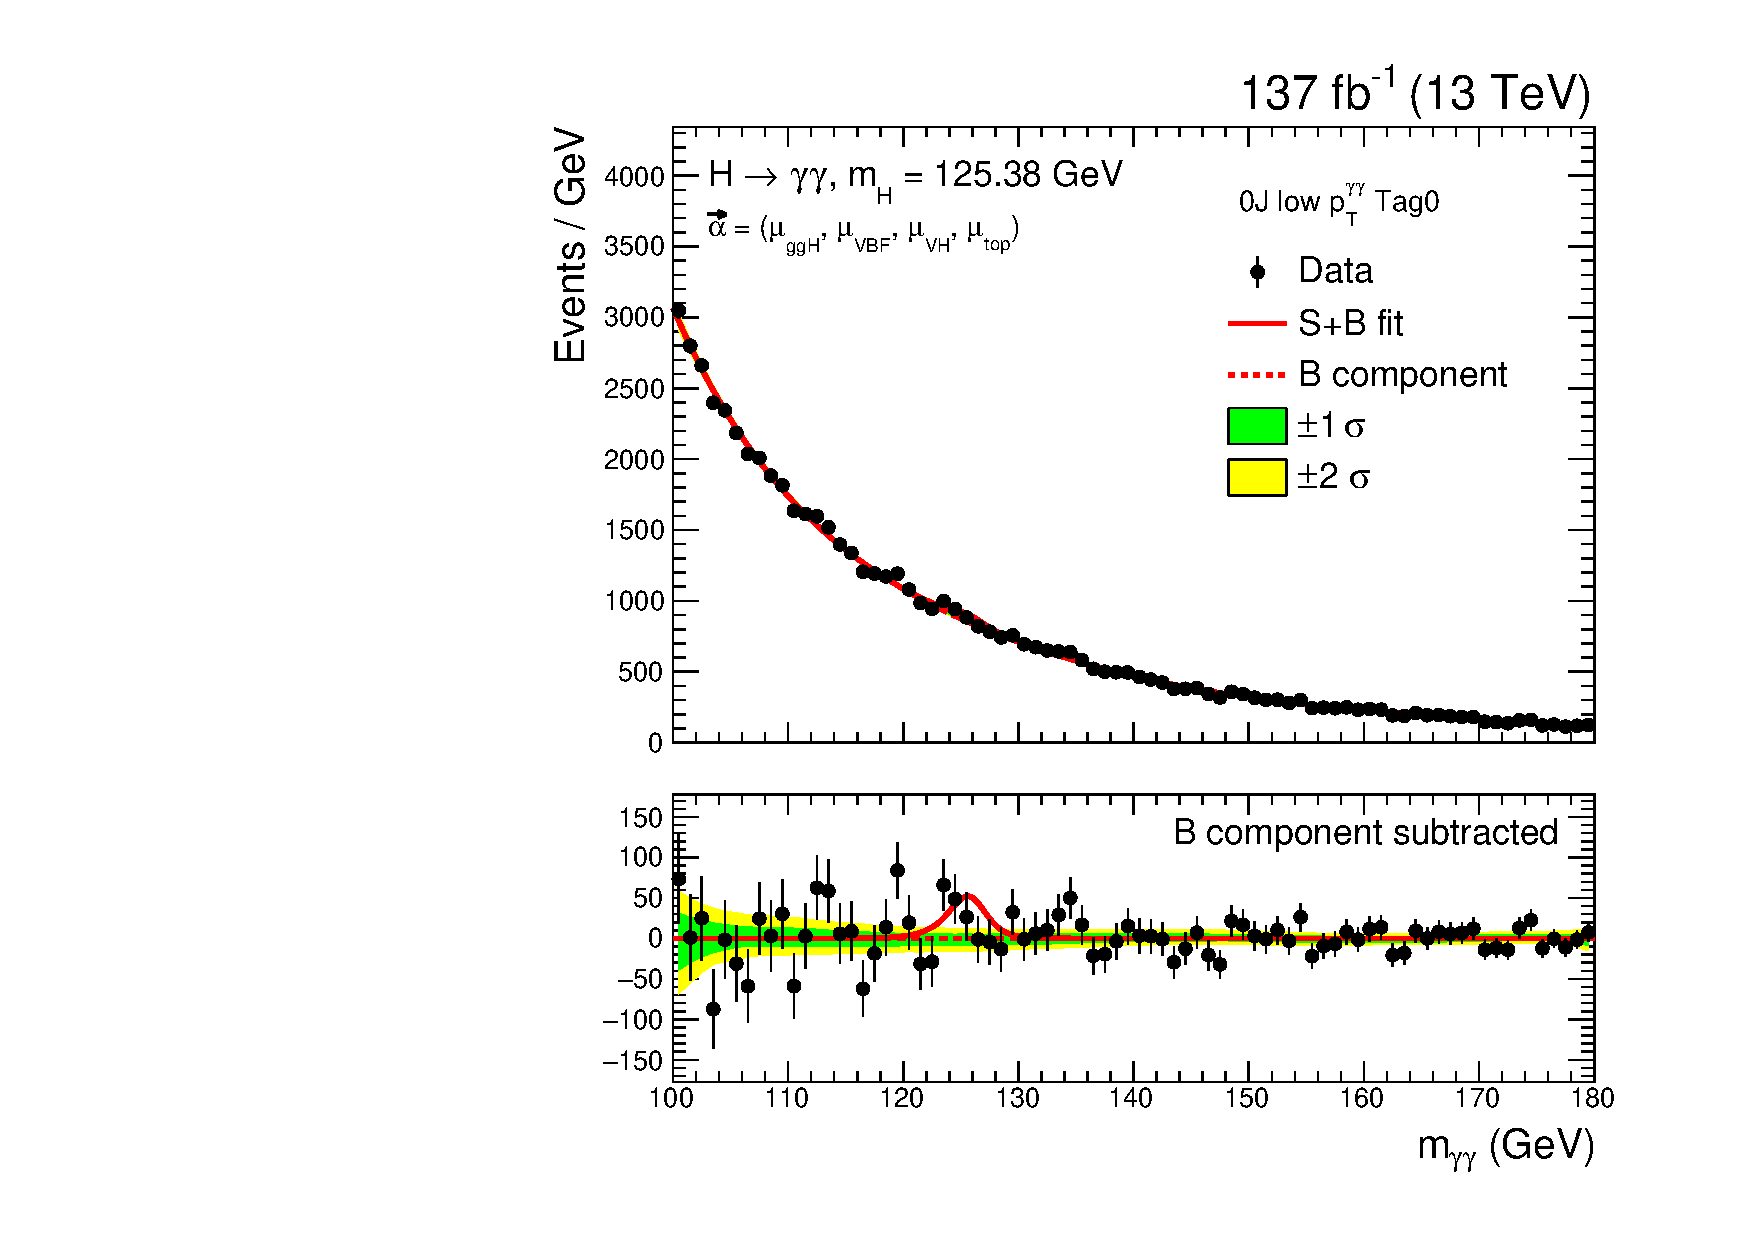
\includegraphics[width=.32\linewidth]{Figures/app_sb_models/RECO_0J_PTH_0_10_Tag0_CMS_hgg_mass.pdf}
  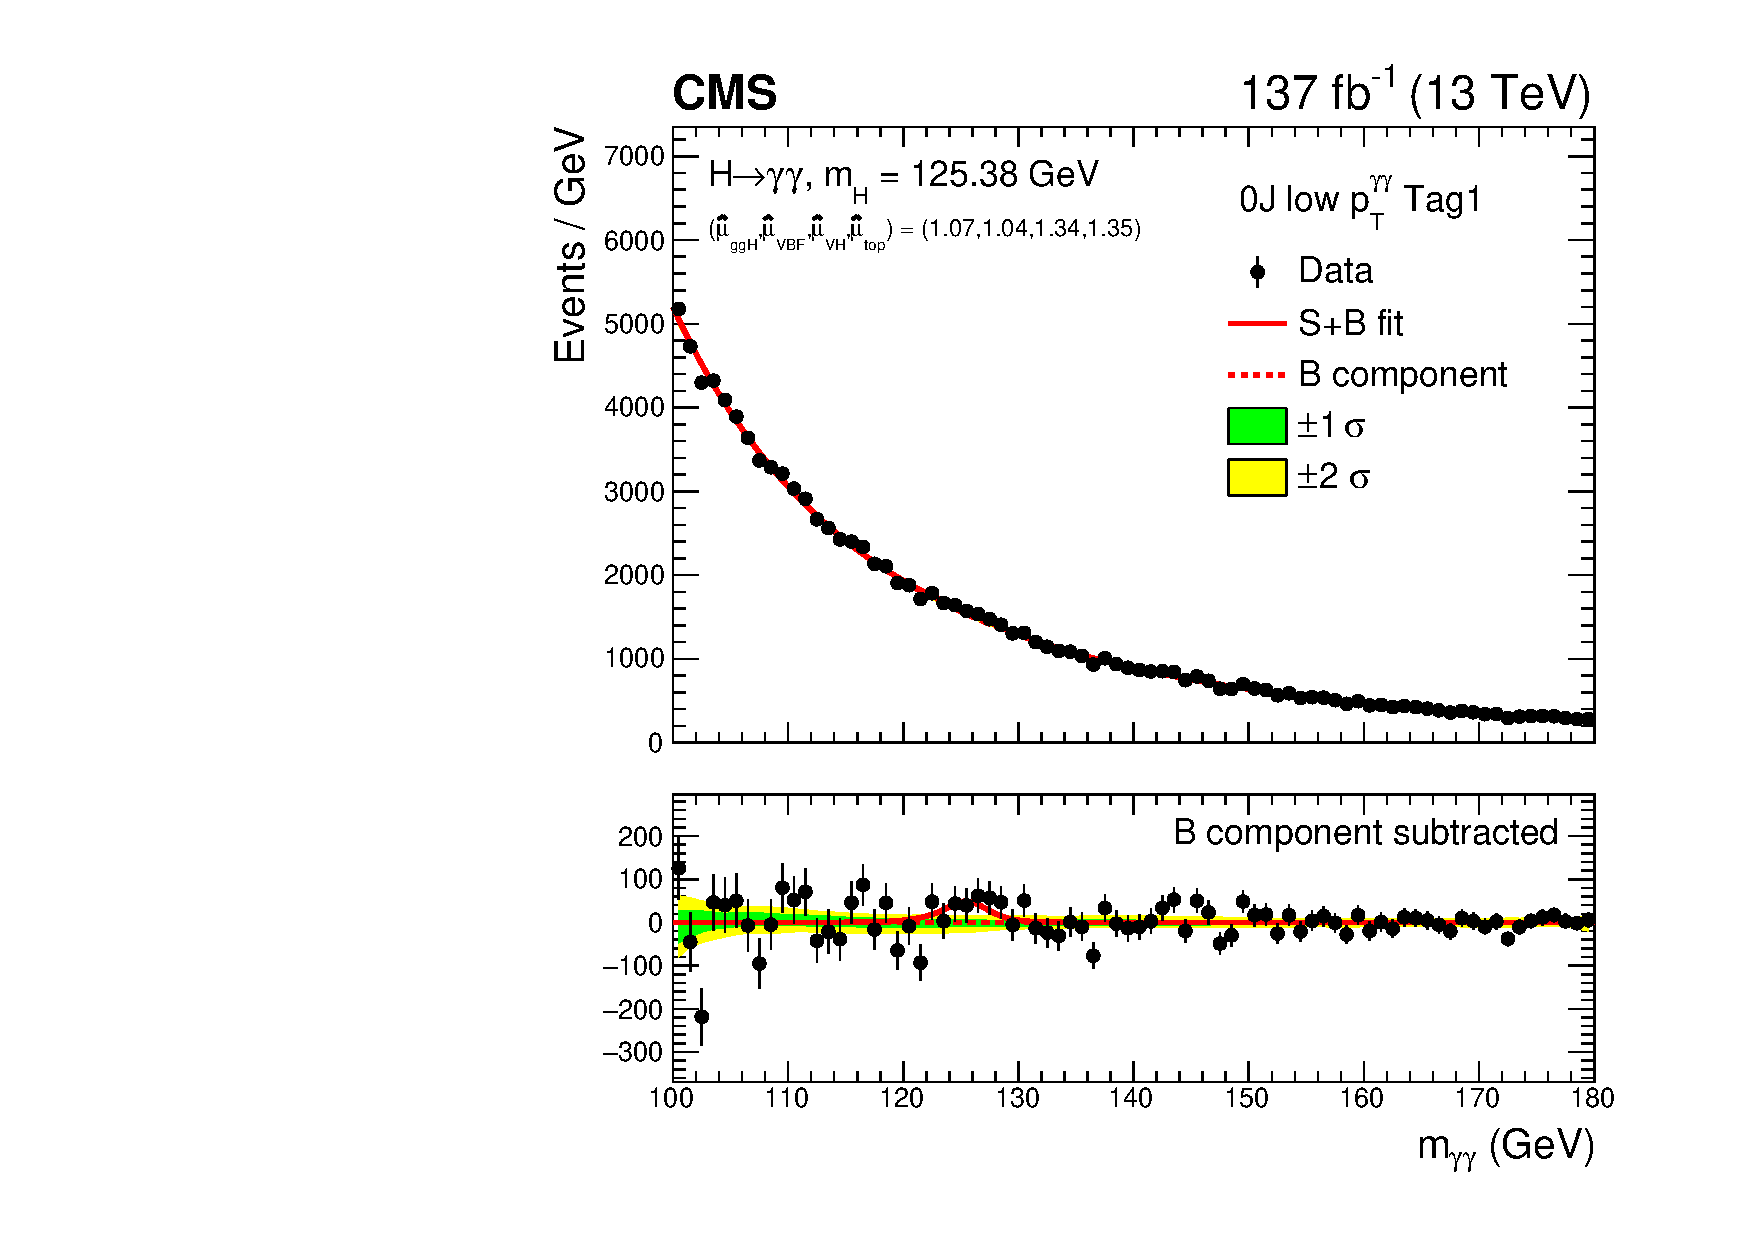
\includegraphics[width=.32\linewidth]{Figures/app_sb_models/RECO_0J_PTH_0_10_Tag1_CMS_hgg_mass.pdf}
  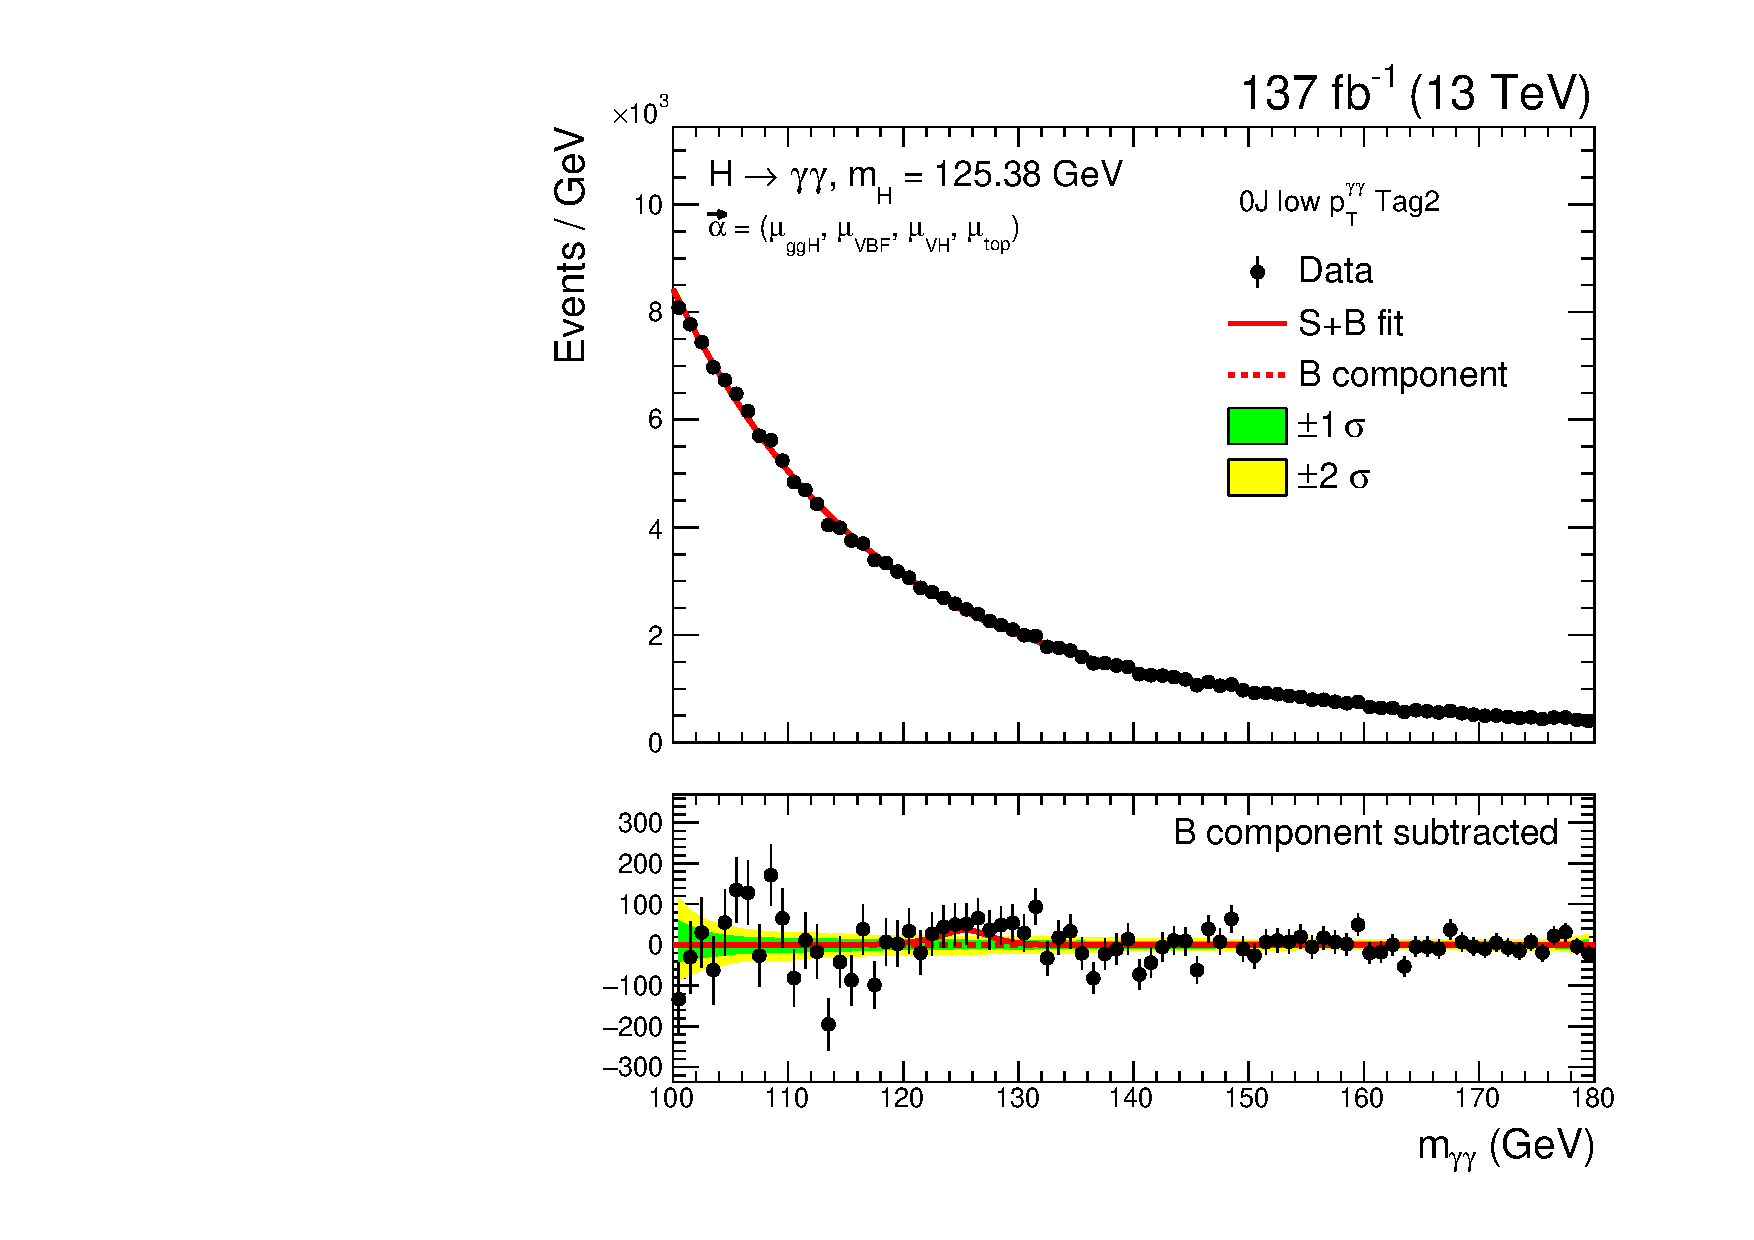
\includegraphics[width=.32\linewidth]{Figures/app_sb_models/RECO_0J_PTH_0_10_Tag2_CMS_hgg_mass.pdf}
  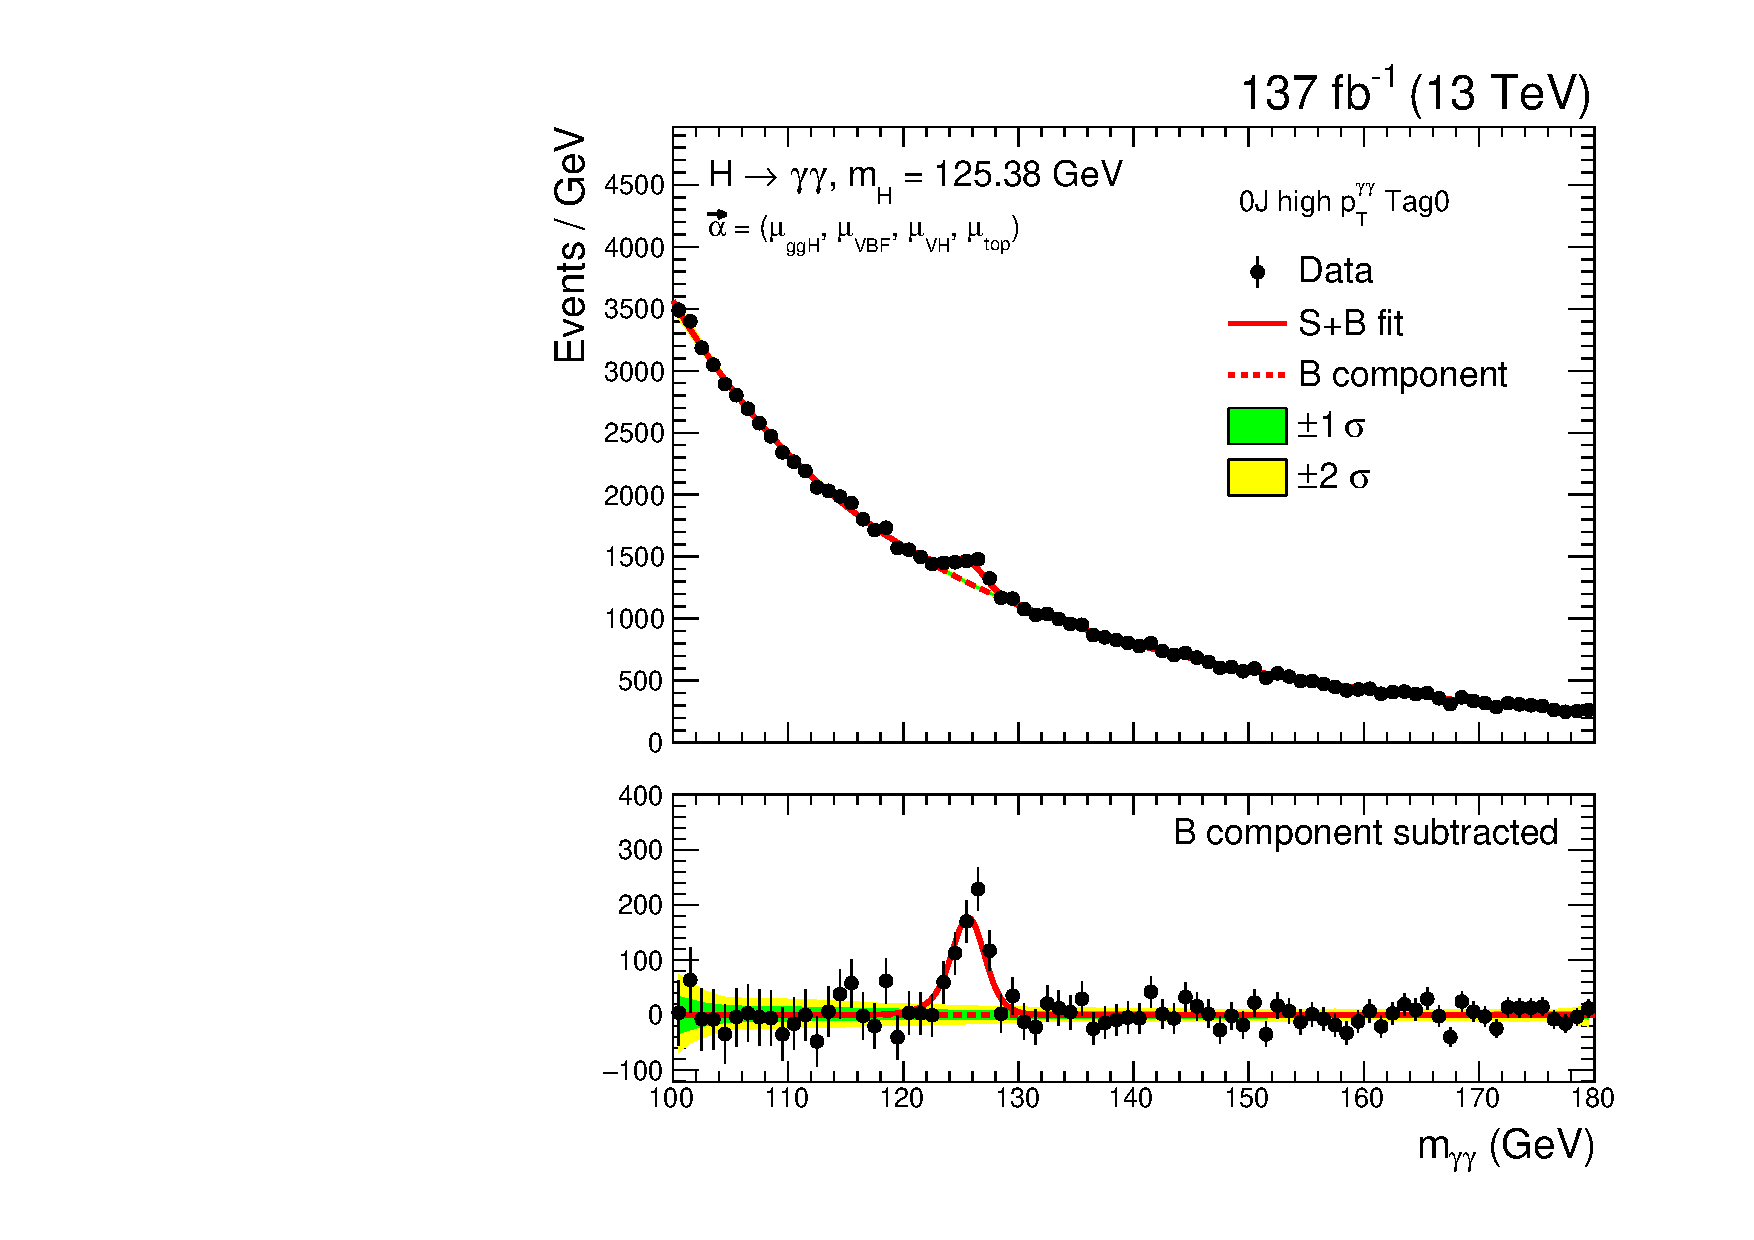
\includegraphics[width=.32\linewidth]{Figures/app_sb_models/RECO_0J_PTH_GT10_Tag0_CMS_hgg_mass.pdf}
  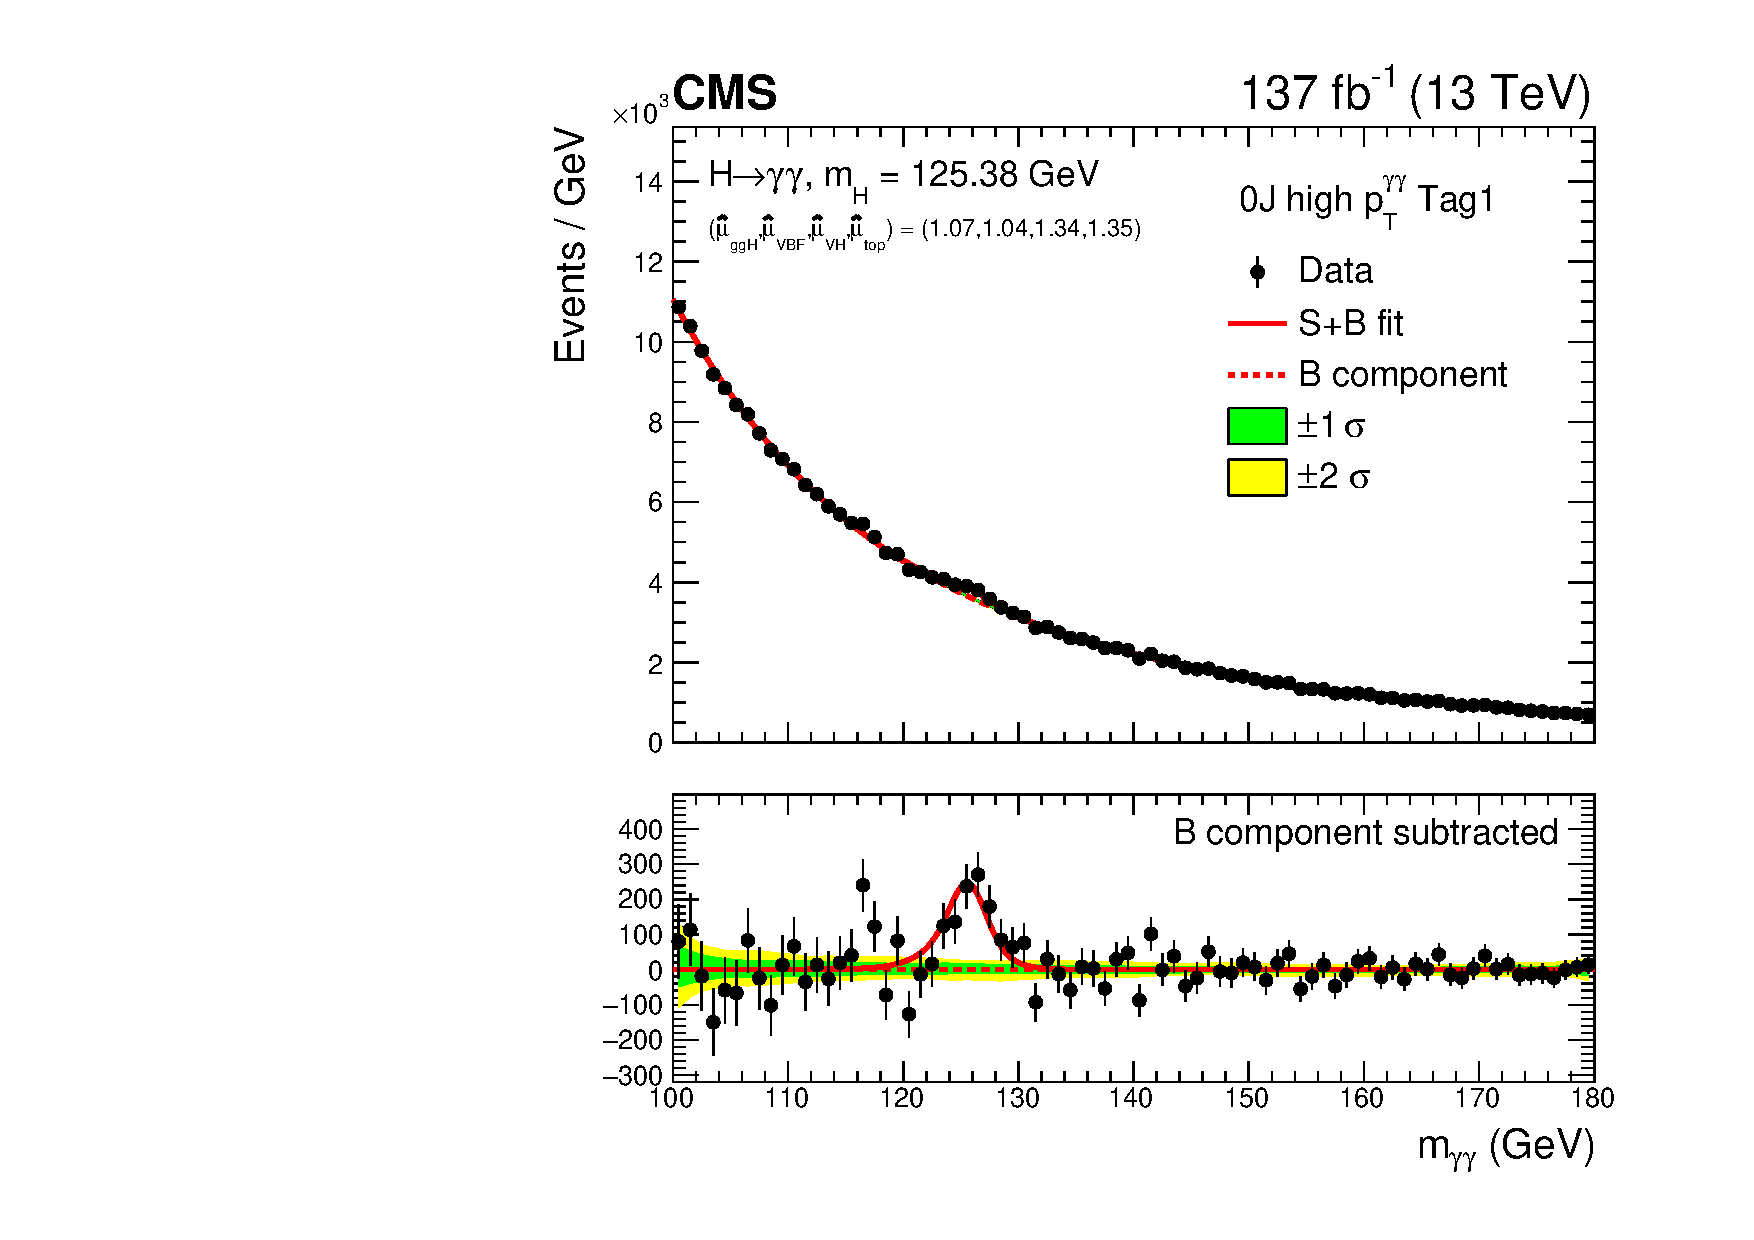
\includegraphics[width=.32\linewidth]{Figures/app_sb_models/RECO_0J_PTH_GT10_Tag1_CMS_hgg_mass.pdf}
  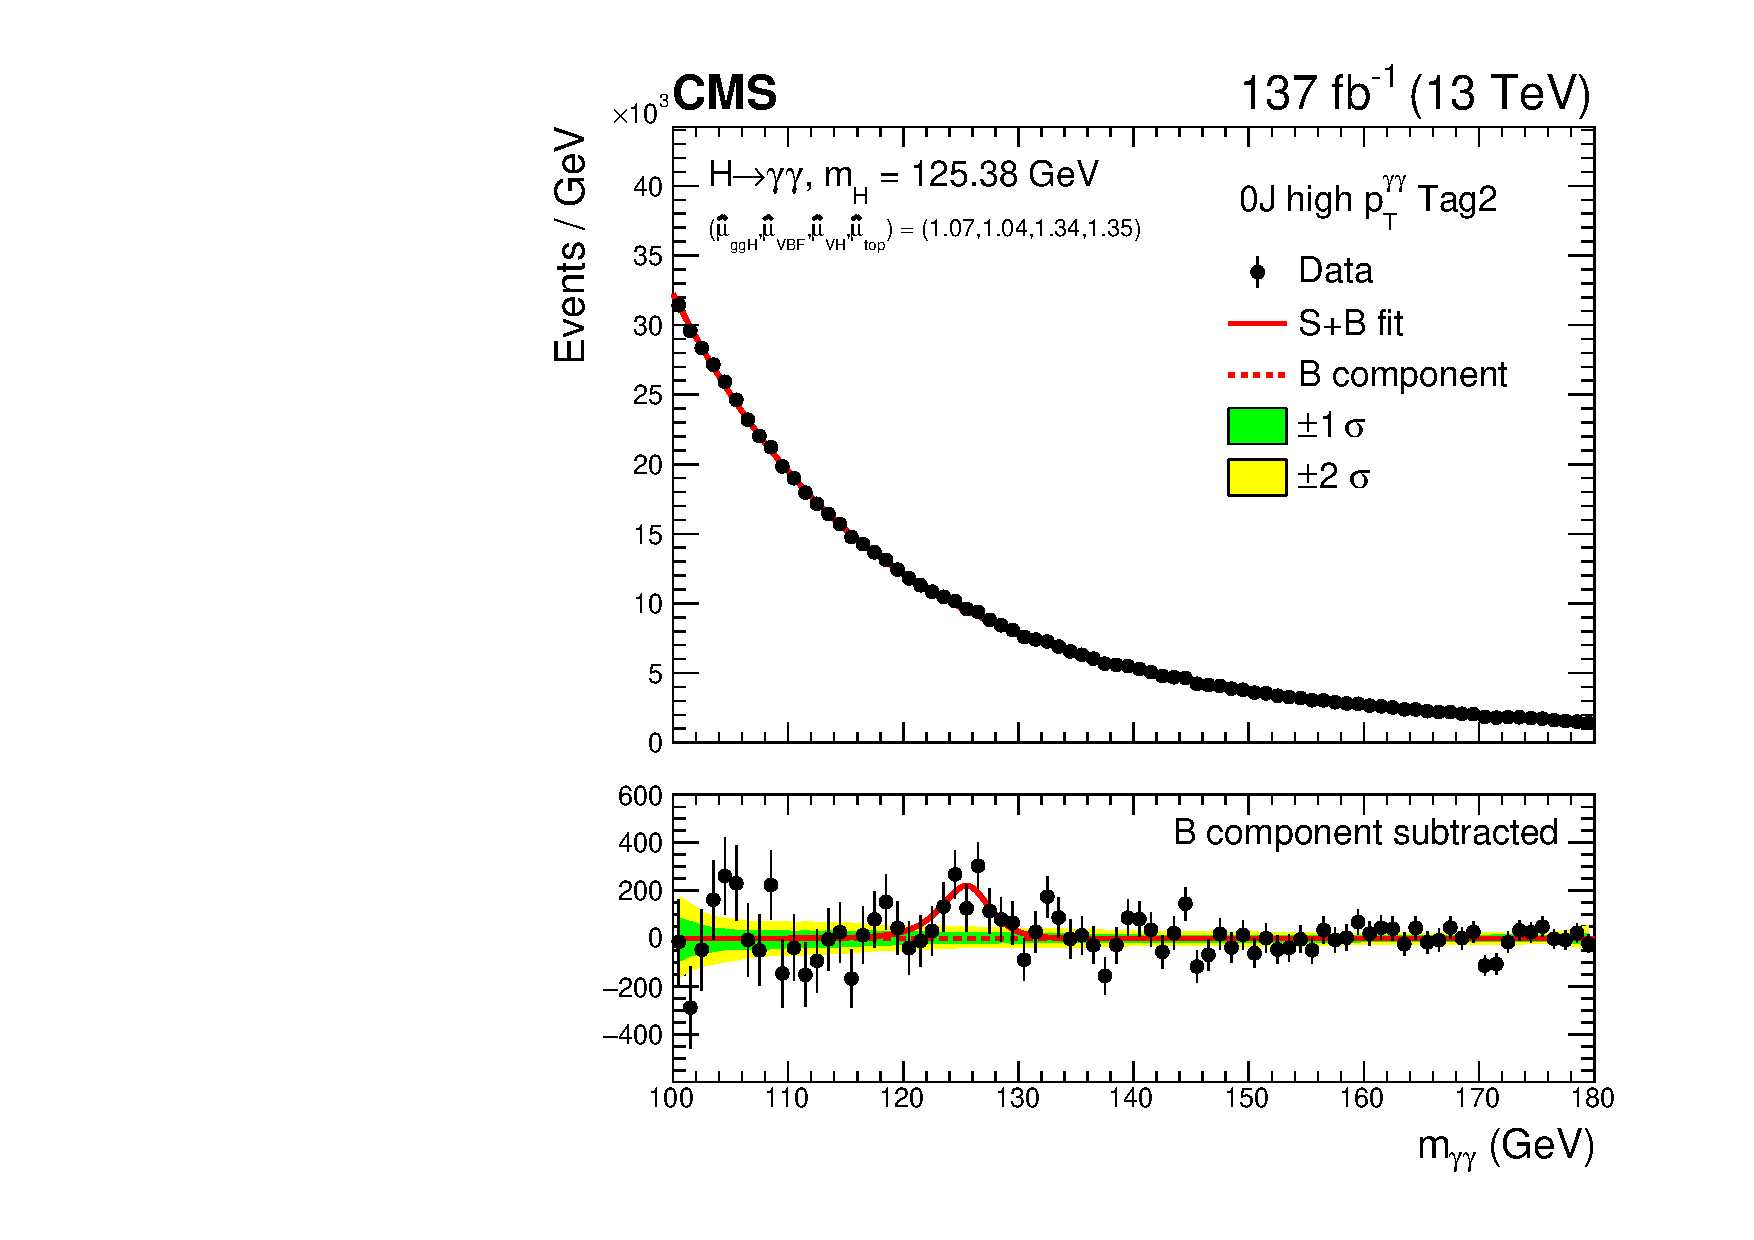
\includegraphics[width=.32\linewidth]{Figures/app_sb_models/RECO_0J_PTH_GT10_Tag2_CMS_hgg_mass.pdf}
  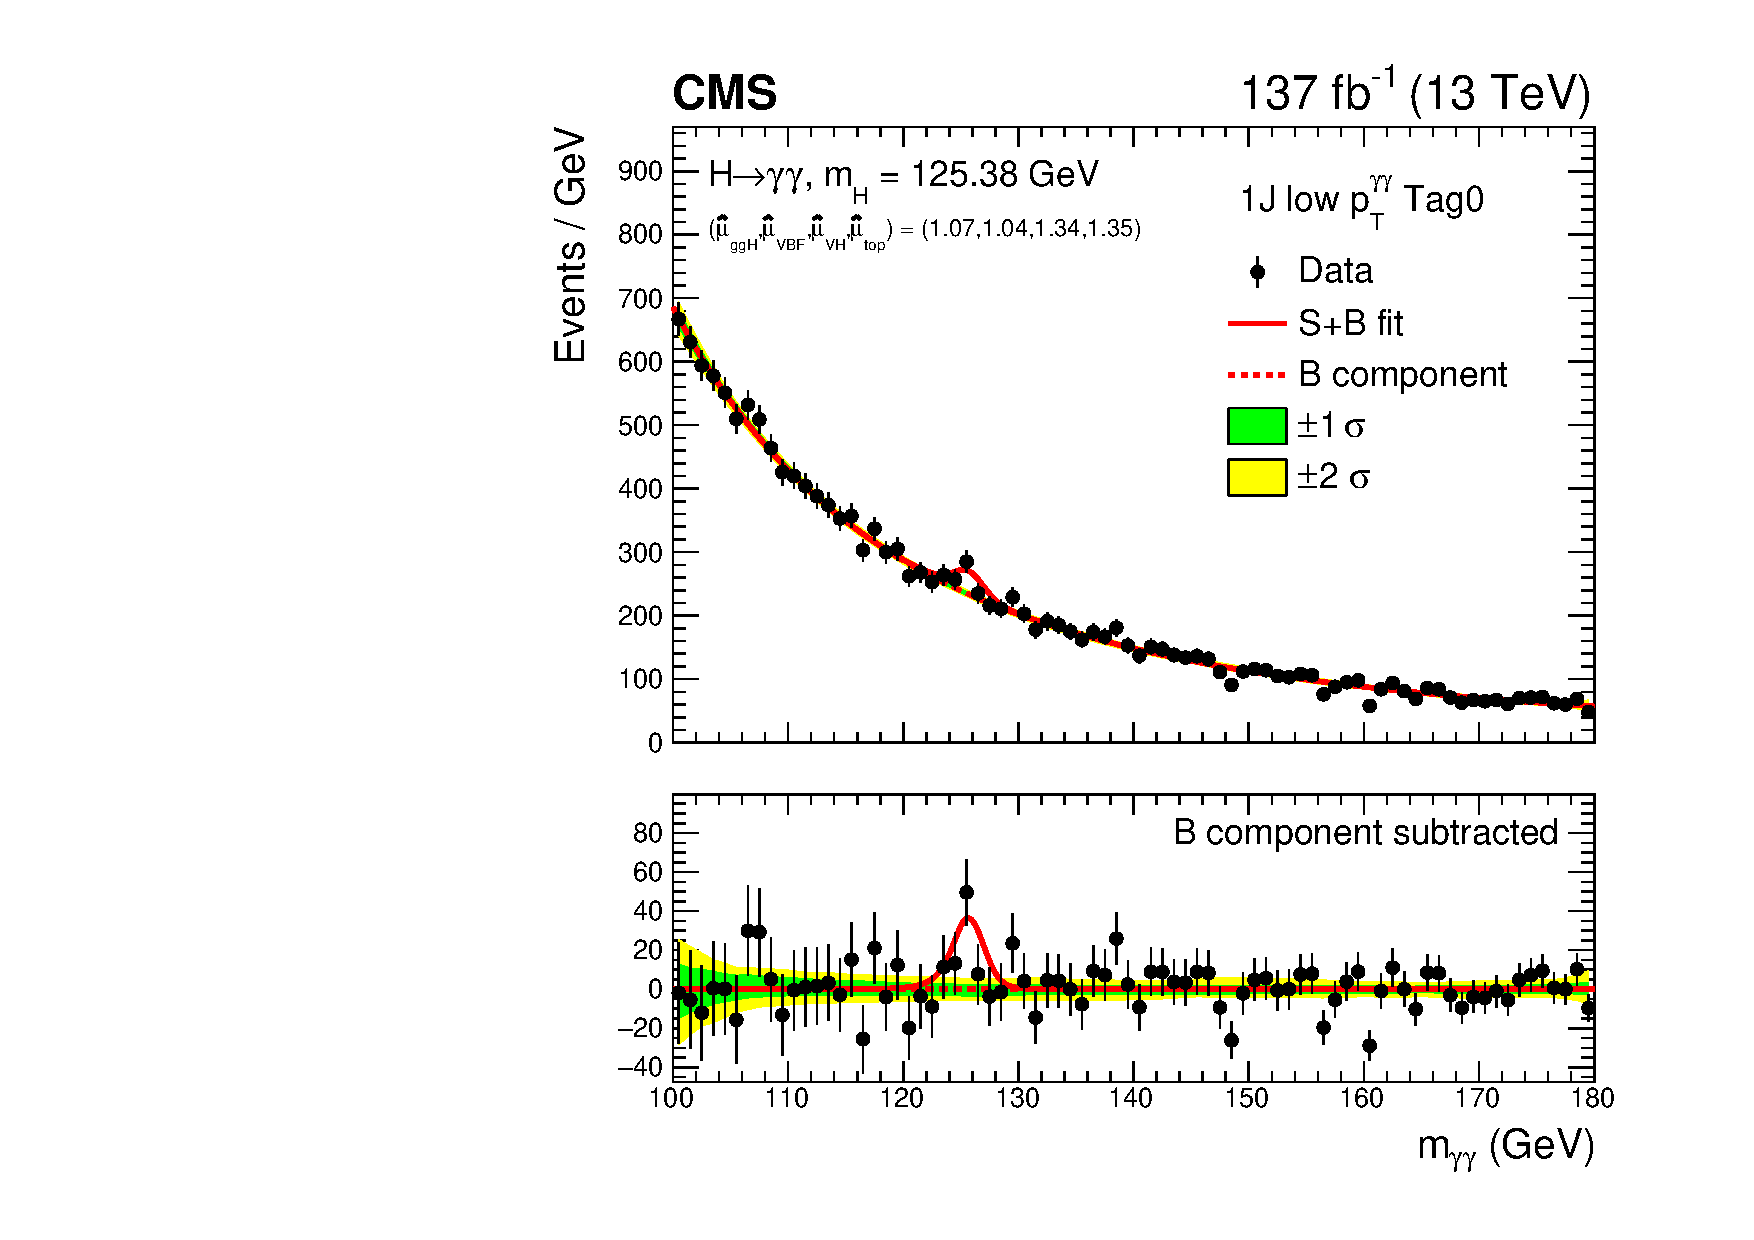
\includegraphics[width=.32\linewidth]{Figures/app_sb_models/RECO_1J_PTH_0_60_Tag0_CMS_hgg_mass.pdf}
  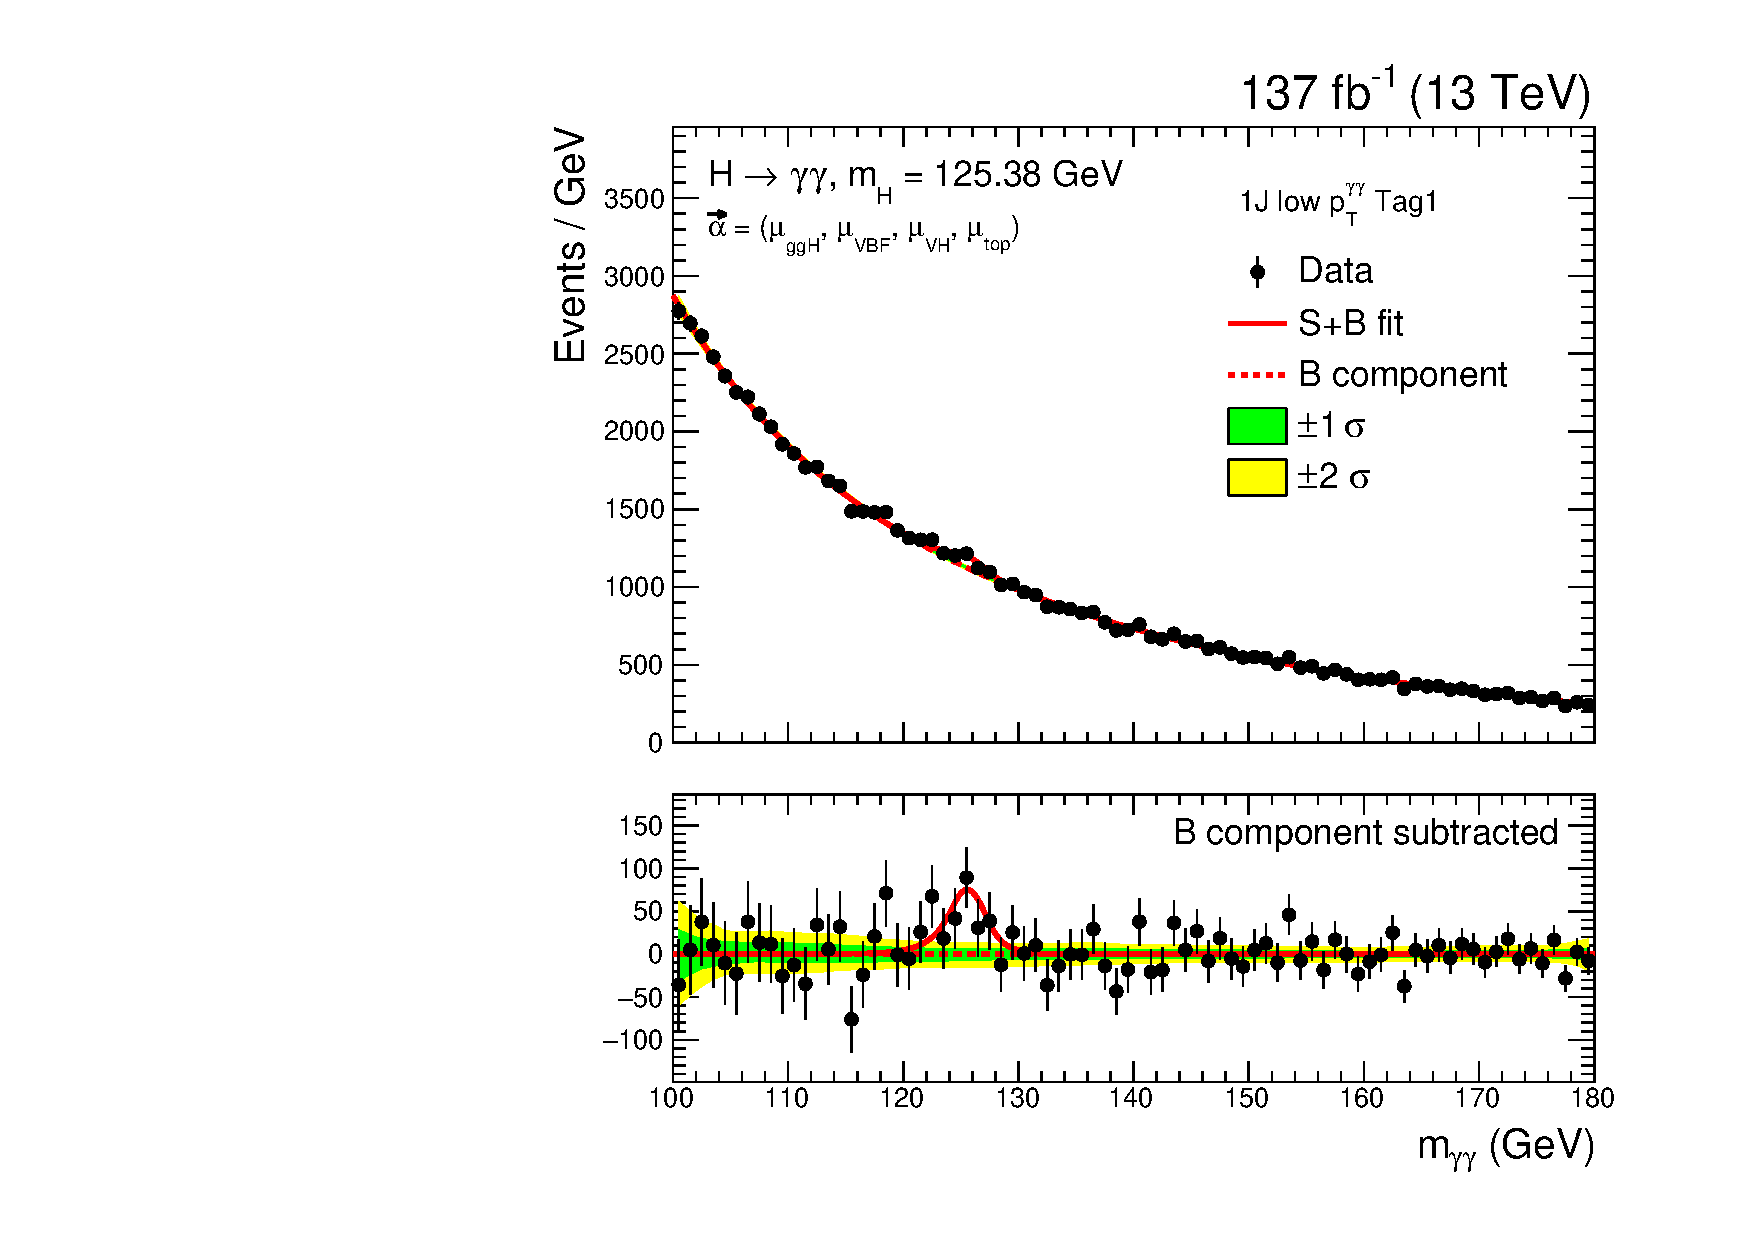
\includegraphics[width=.32\linewidth]{Figures/app_sb_models/RECO_1J_PTH_0_60_Tag1_CMS_hgg_mass.pdf}
  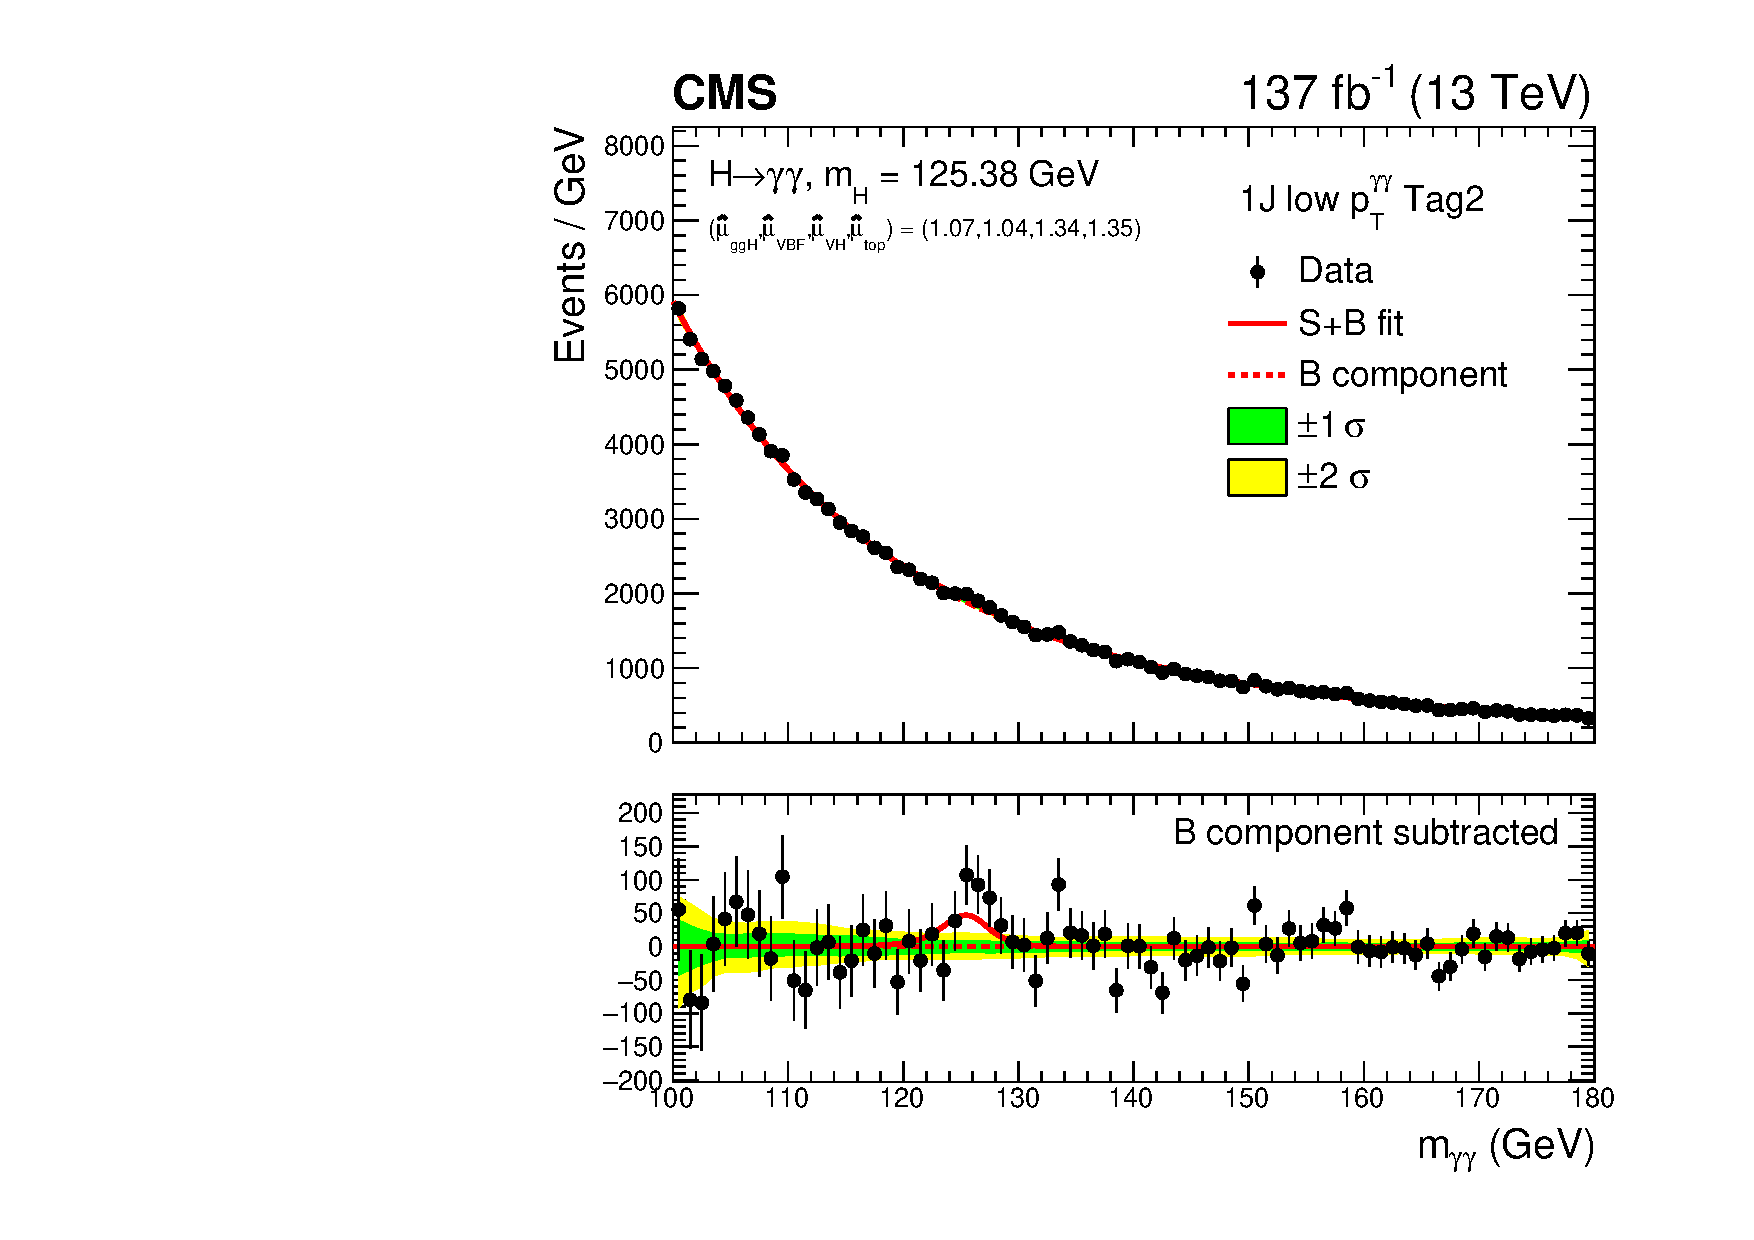
\includegraphics[width=.32\linewidth]{Figures/app_sb_models/RECO_1J_PTH_0_60_Tag2_CMS_hgg_mass.pdf}  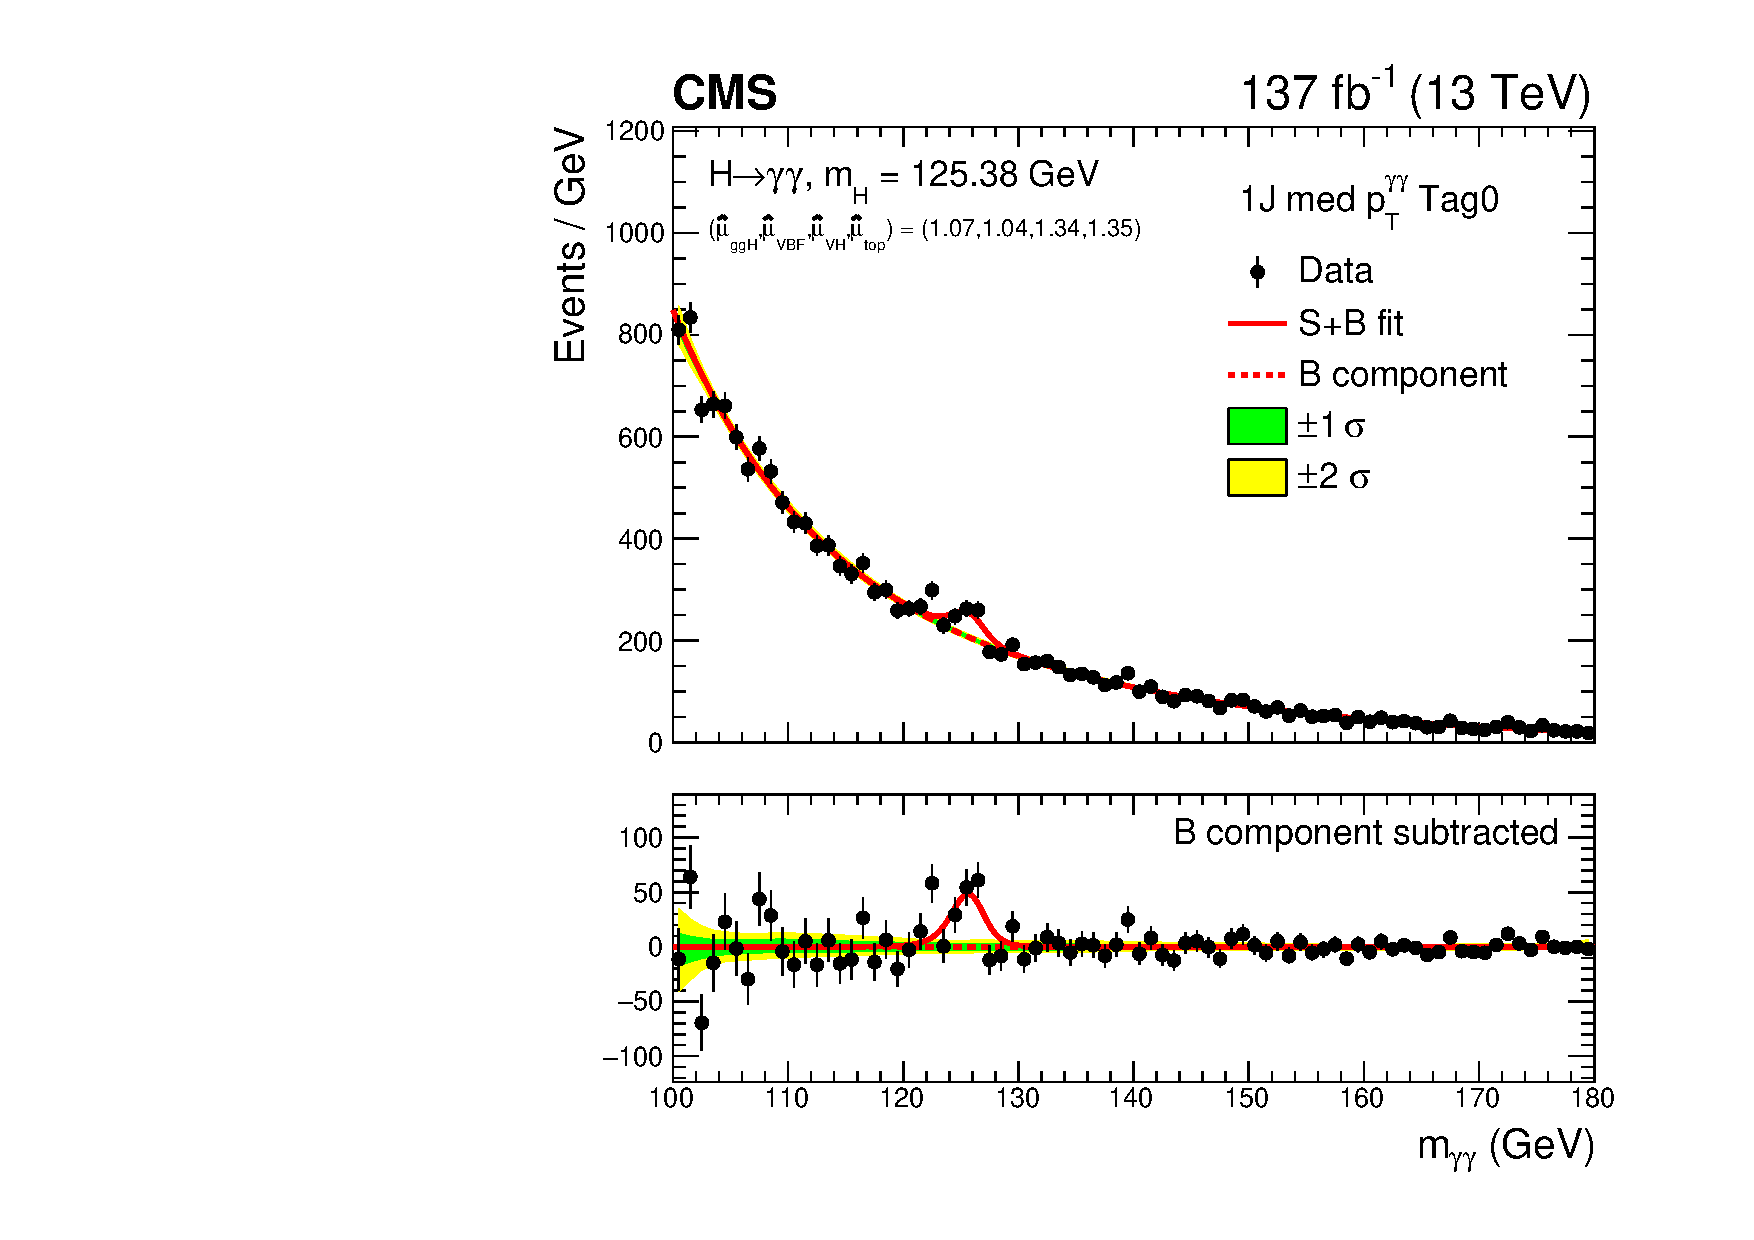
\includegraphics[width=.32\linewidth]{Figures/app_sb_models/RECO_1J_PTH_60_120_Tag0_CMS_hgg_mass.pdf}
  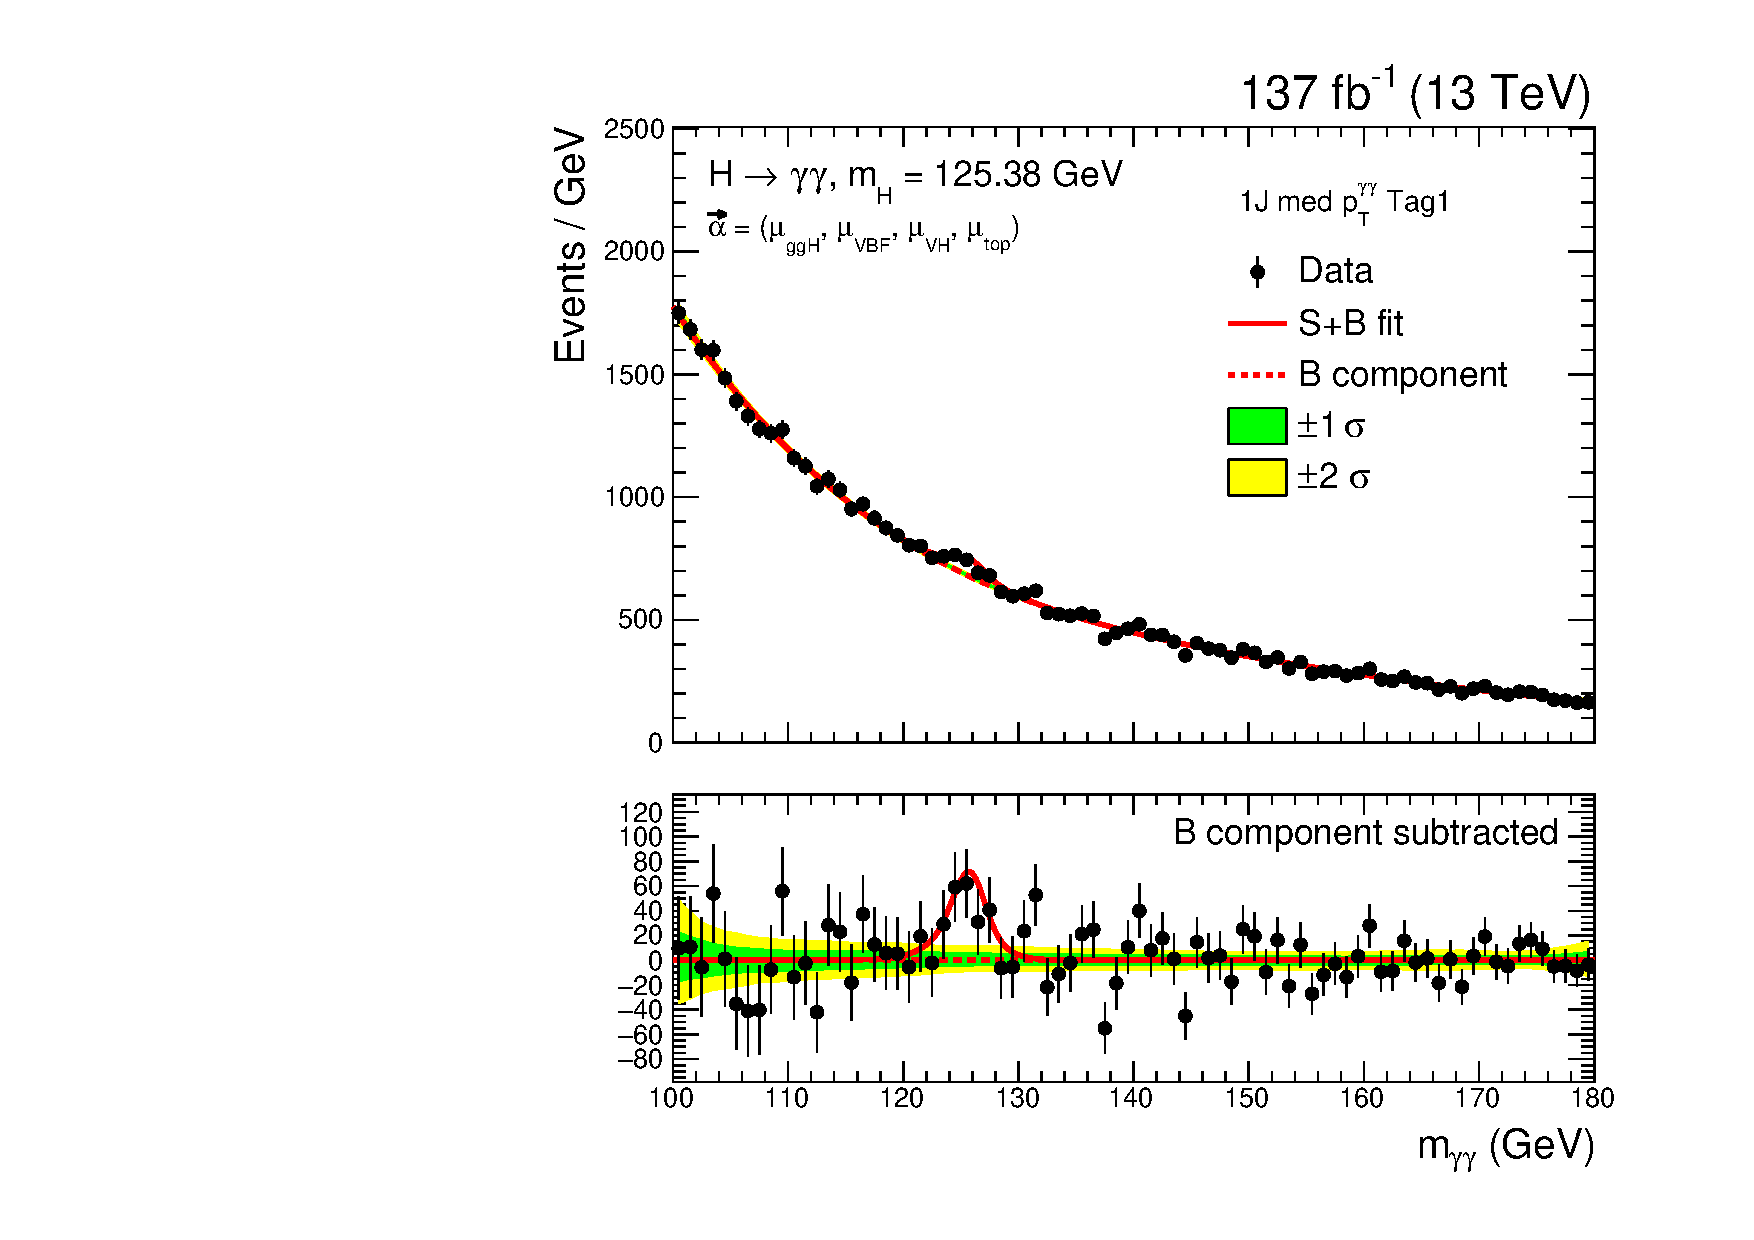
\includegraphics[width=.32\linewidth]{Figures/app_sb_models/RECO_1J_PTH_60_120_Tag1_CMS_hgg_mass.pdf}
  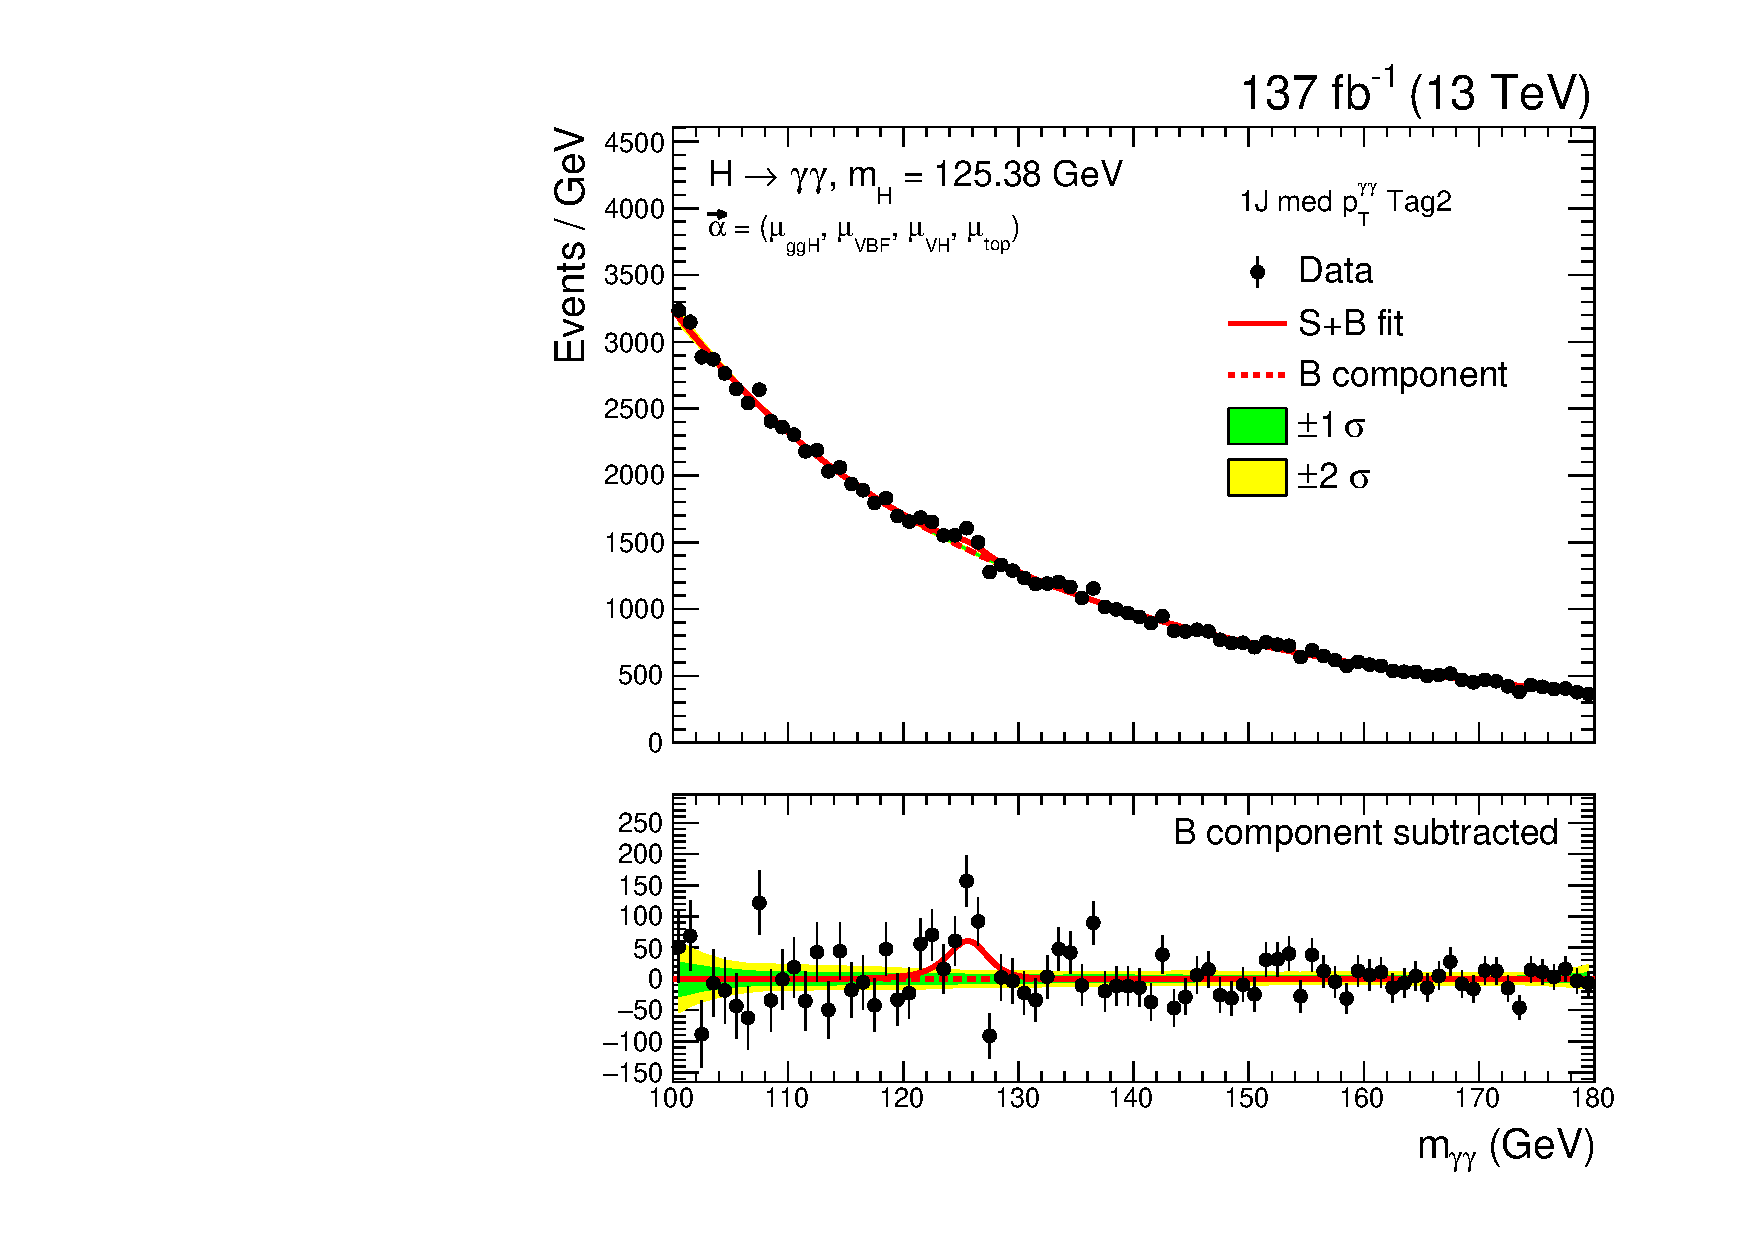
\includegraphics[width=.32\linewidth]{Figures/app_sb_models/RECO_1J_PTH_60_120_Tag2_CMS_hgg_mass.pdf}
  \caption[Observed diphoton mass distributions: ggH 0J and ggH 1J]
  {
    Data points (black) and the best-fit signal-plus-background model for the individual analysis categories targeting a number of ggH STXS regions. The best-fit model corresponds to the per-production mode signal strength fit. The solid red line shows the best-fit signal-plus-background model, whereas the dashed line shows the background component only. The one standard deviation (green) and two standard deviation (yellow) bands show the uncertainties in the background component of the fit. The bottom panels in each plot show the residuals after subtraction of this background component.
  }
  \label{fig:diphoton_mass_0}
\end{figure}

\begin{figure}[htbp]
  \centering
  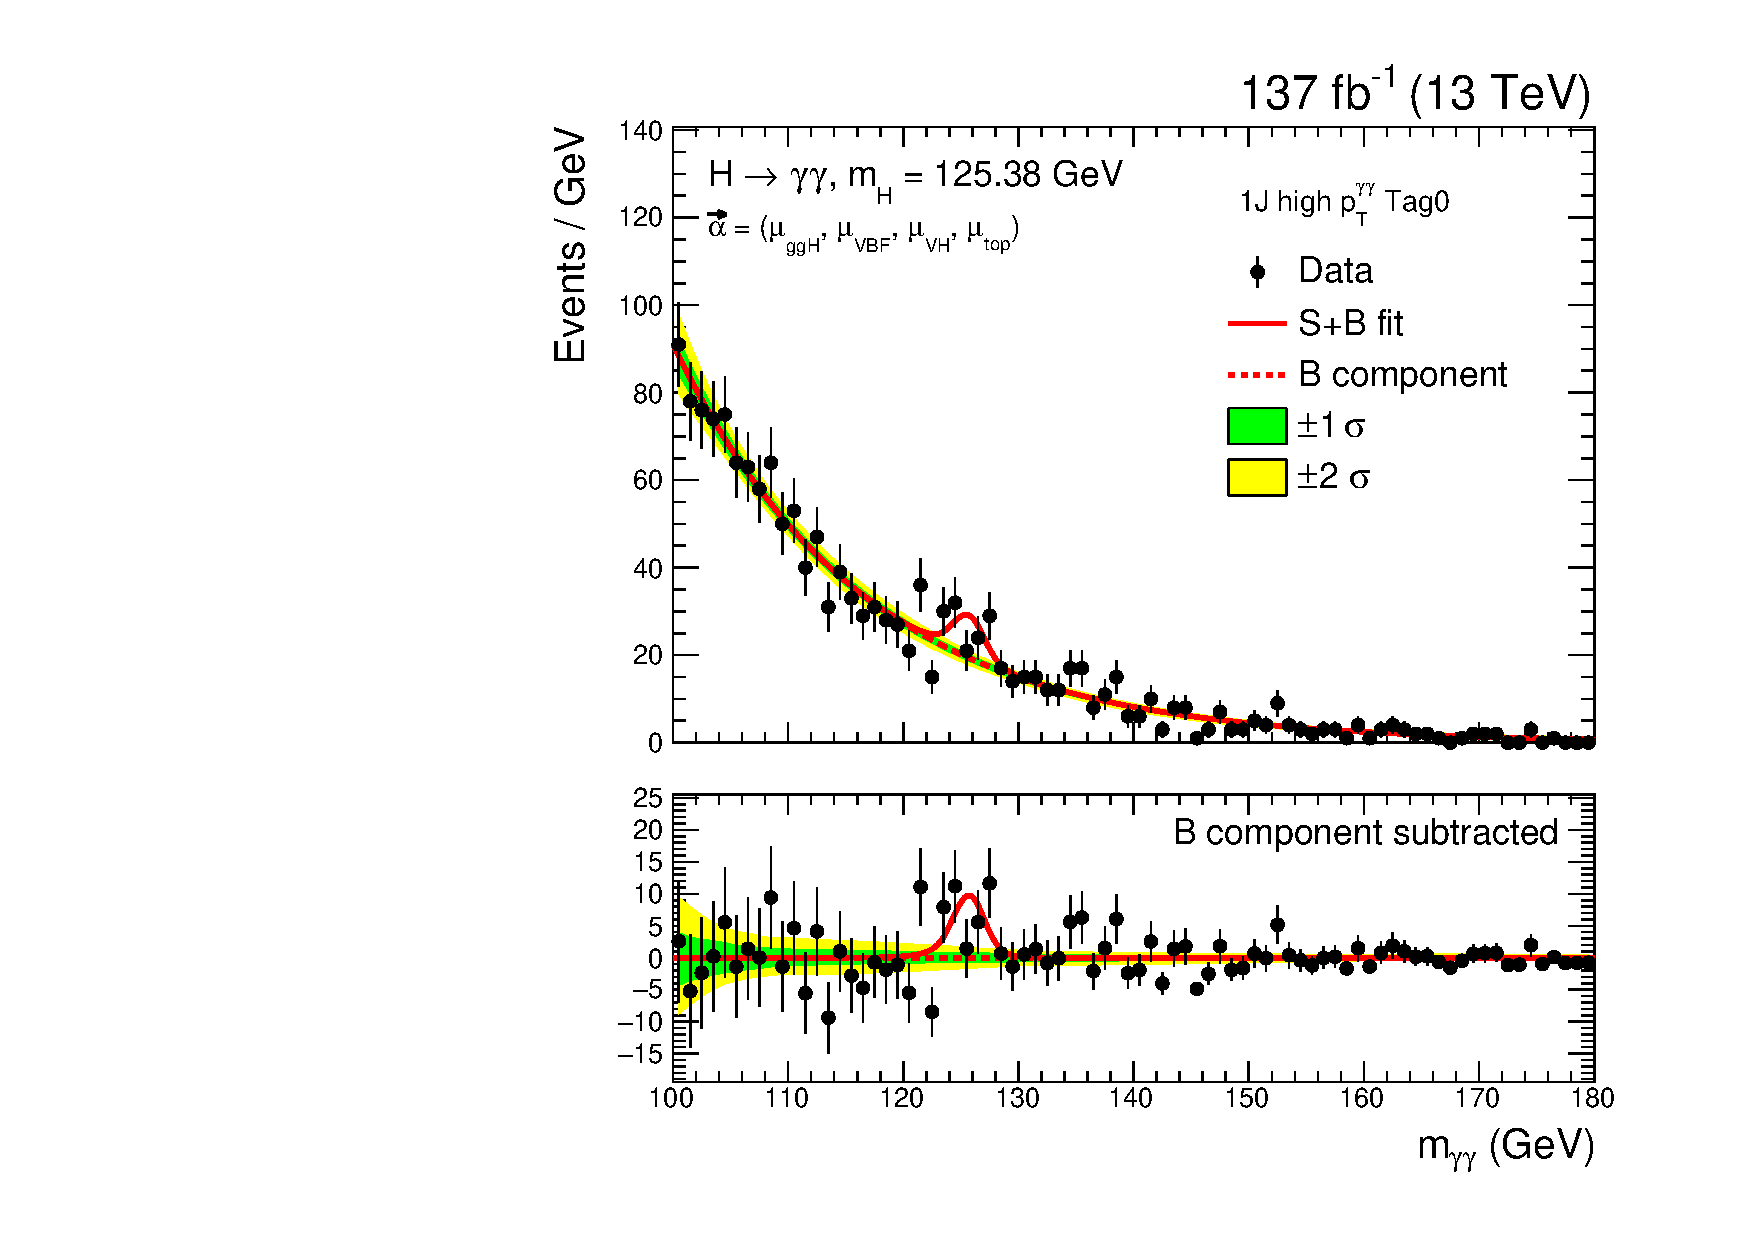
\includegraphics[width=.32\linewidth]{Figures/app_sb_models/RECO_1J_PTH_120_200_Tag0_CMS_hgg_mass.pdf}
  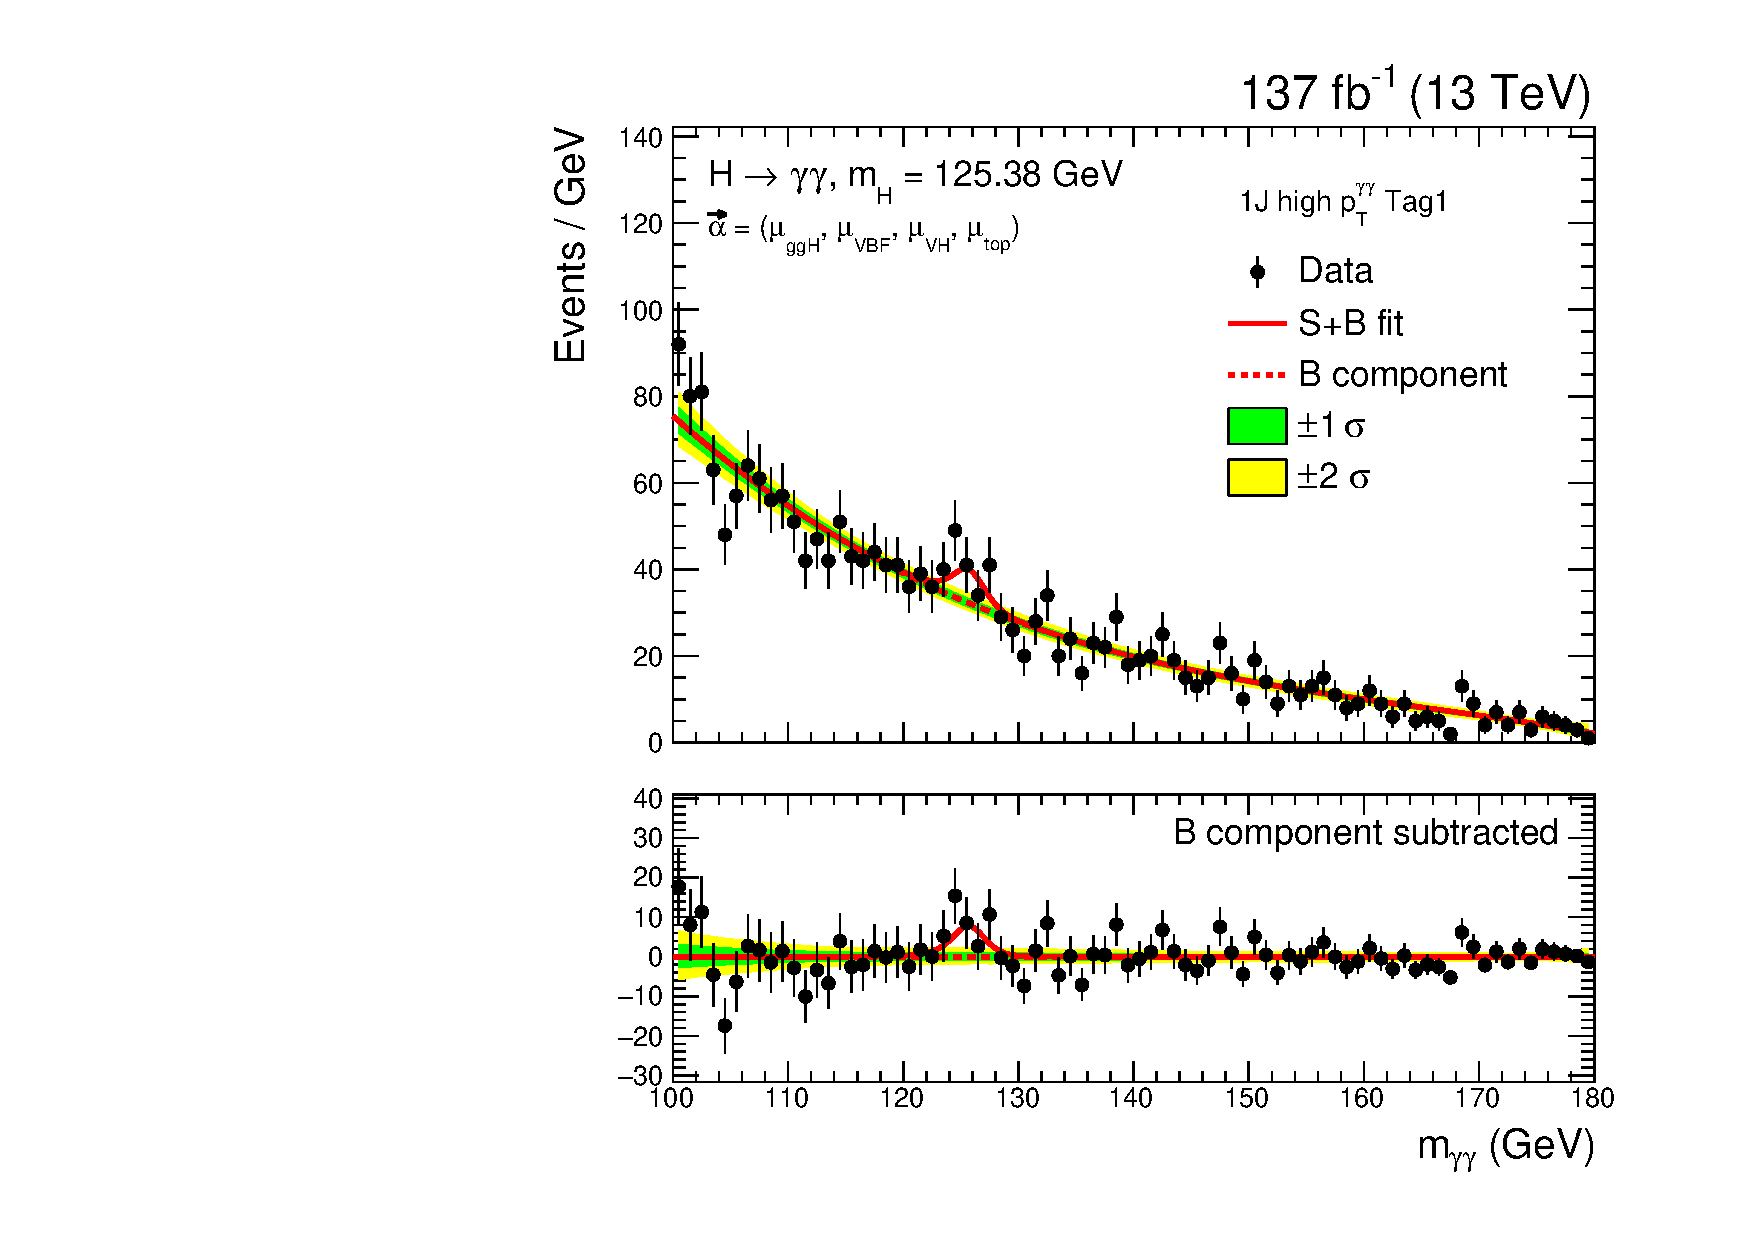
\includegraphics[width=.32\linewidth]{Figures/app_sb_models/RECO_1J_PTH_120_200_Tag1_CMS_hgg_mass.pdf}
  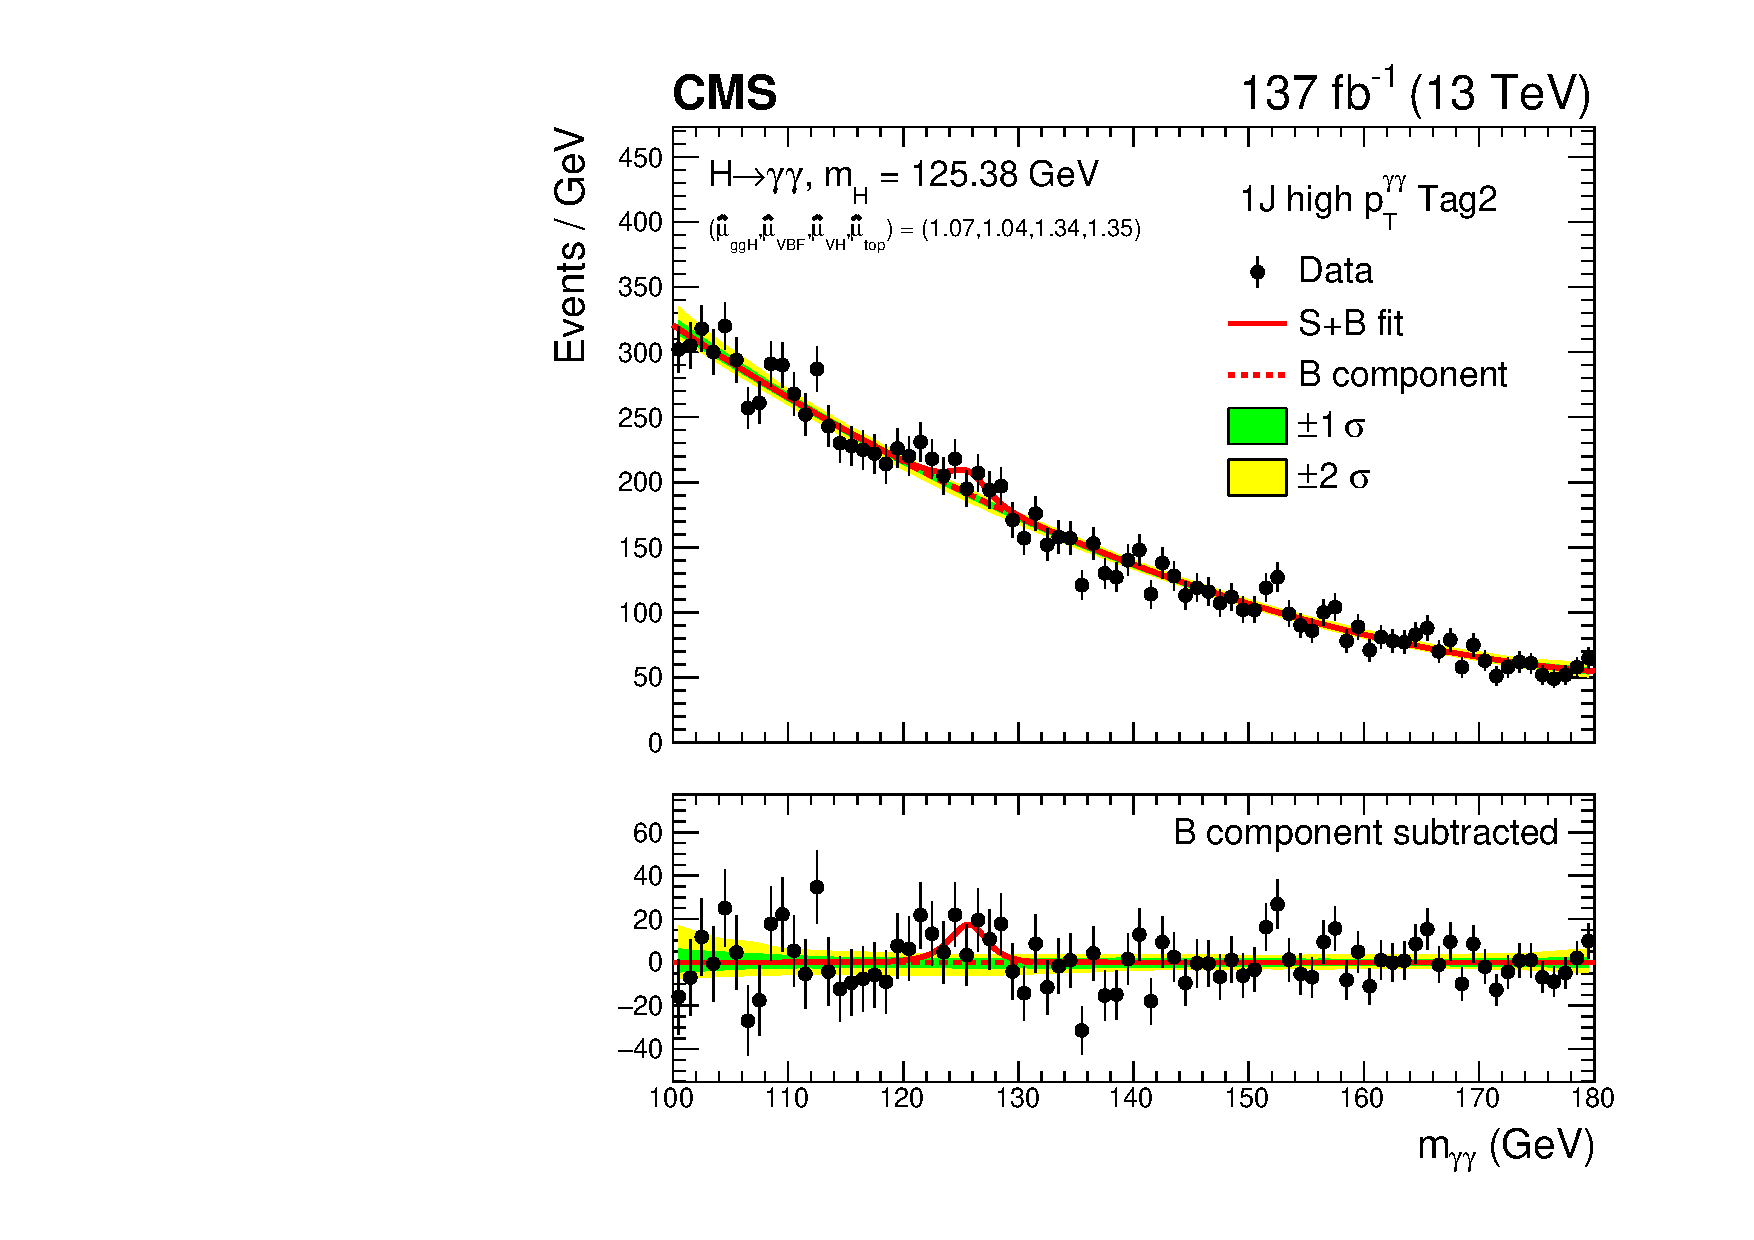
\includegraphics[width=.32\linewidth]{Figures/app_sb_models/RECO_1J_PTH_120_200_Tag2_CMS_hgg_mass.pdf}
  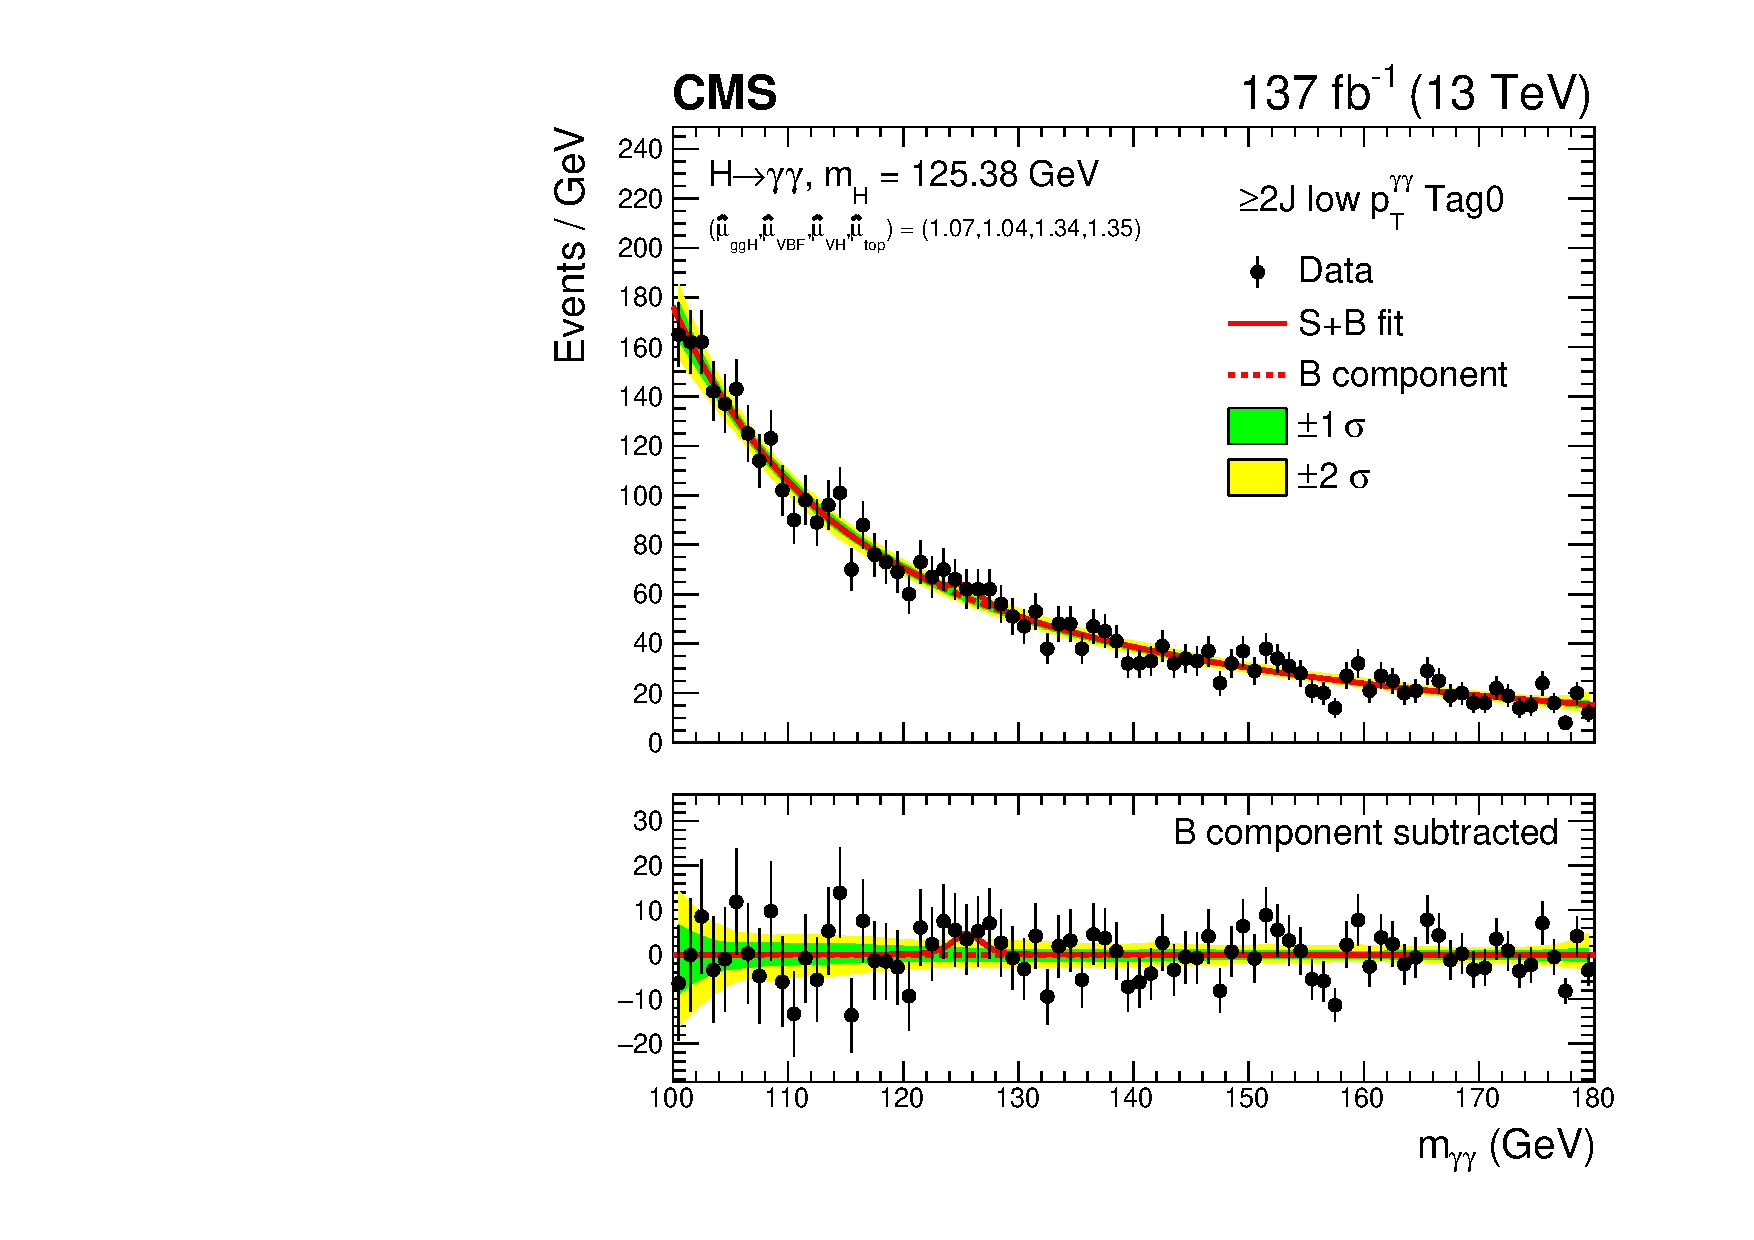
\includegraphics[width=.32\linewidth]{Figures/app_sb_models/RECO_GE2J_PTH_0_60_Tag0_CMS_hgg_mass.pdf}
  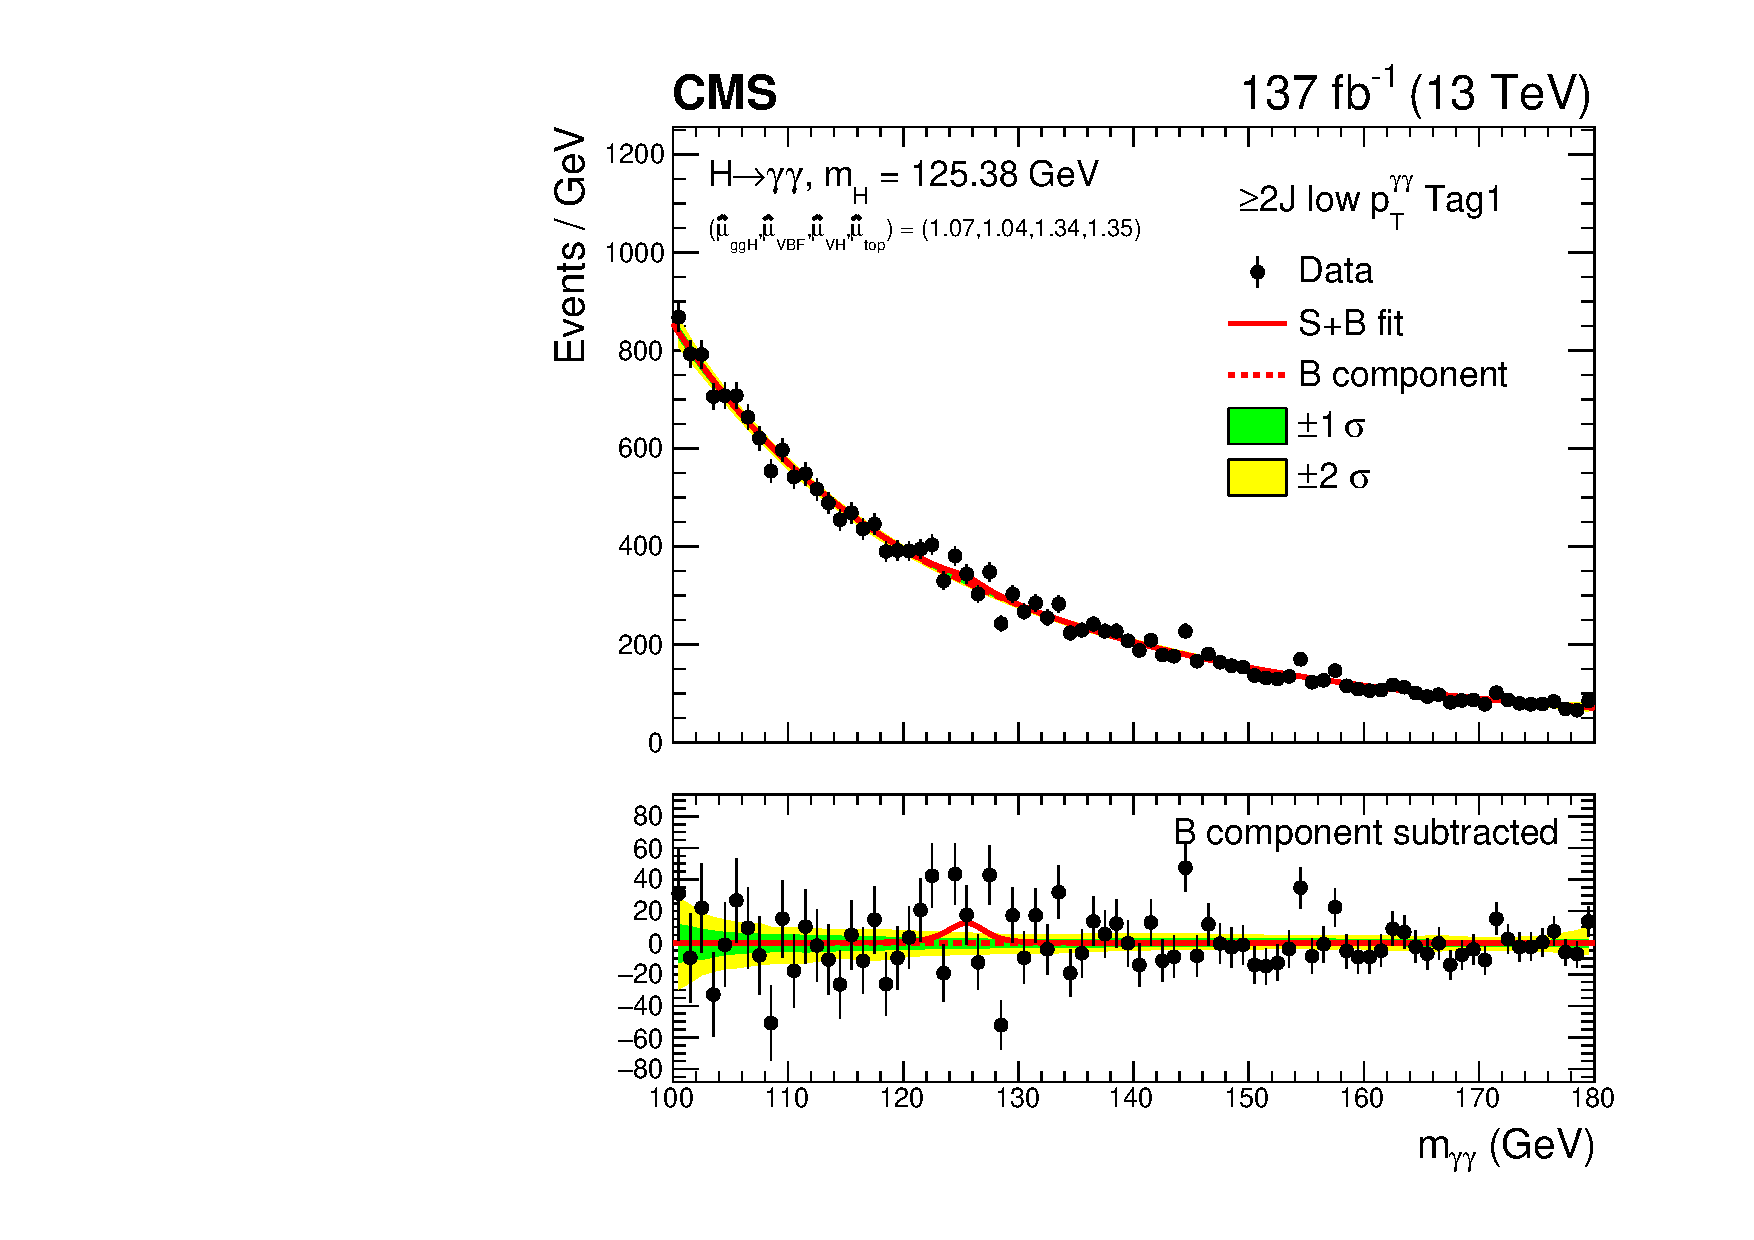
\includegraphics[width=.32\linewidth]{Figures/app_sb_models/RECO_GE2J_PTH_0_60_Tag1_CMS_hgg_mass.pdf}
  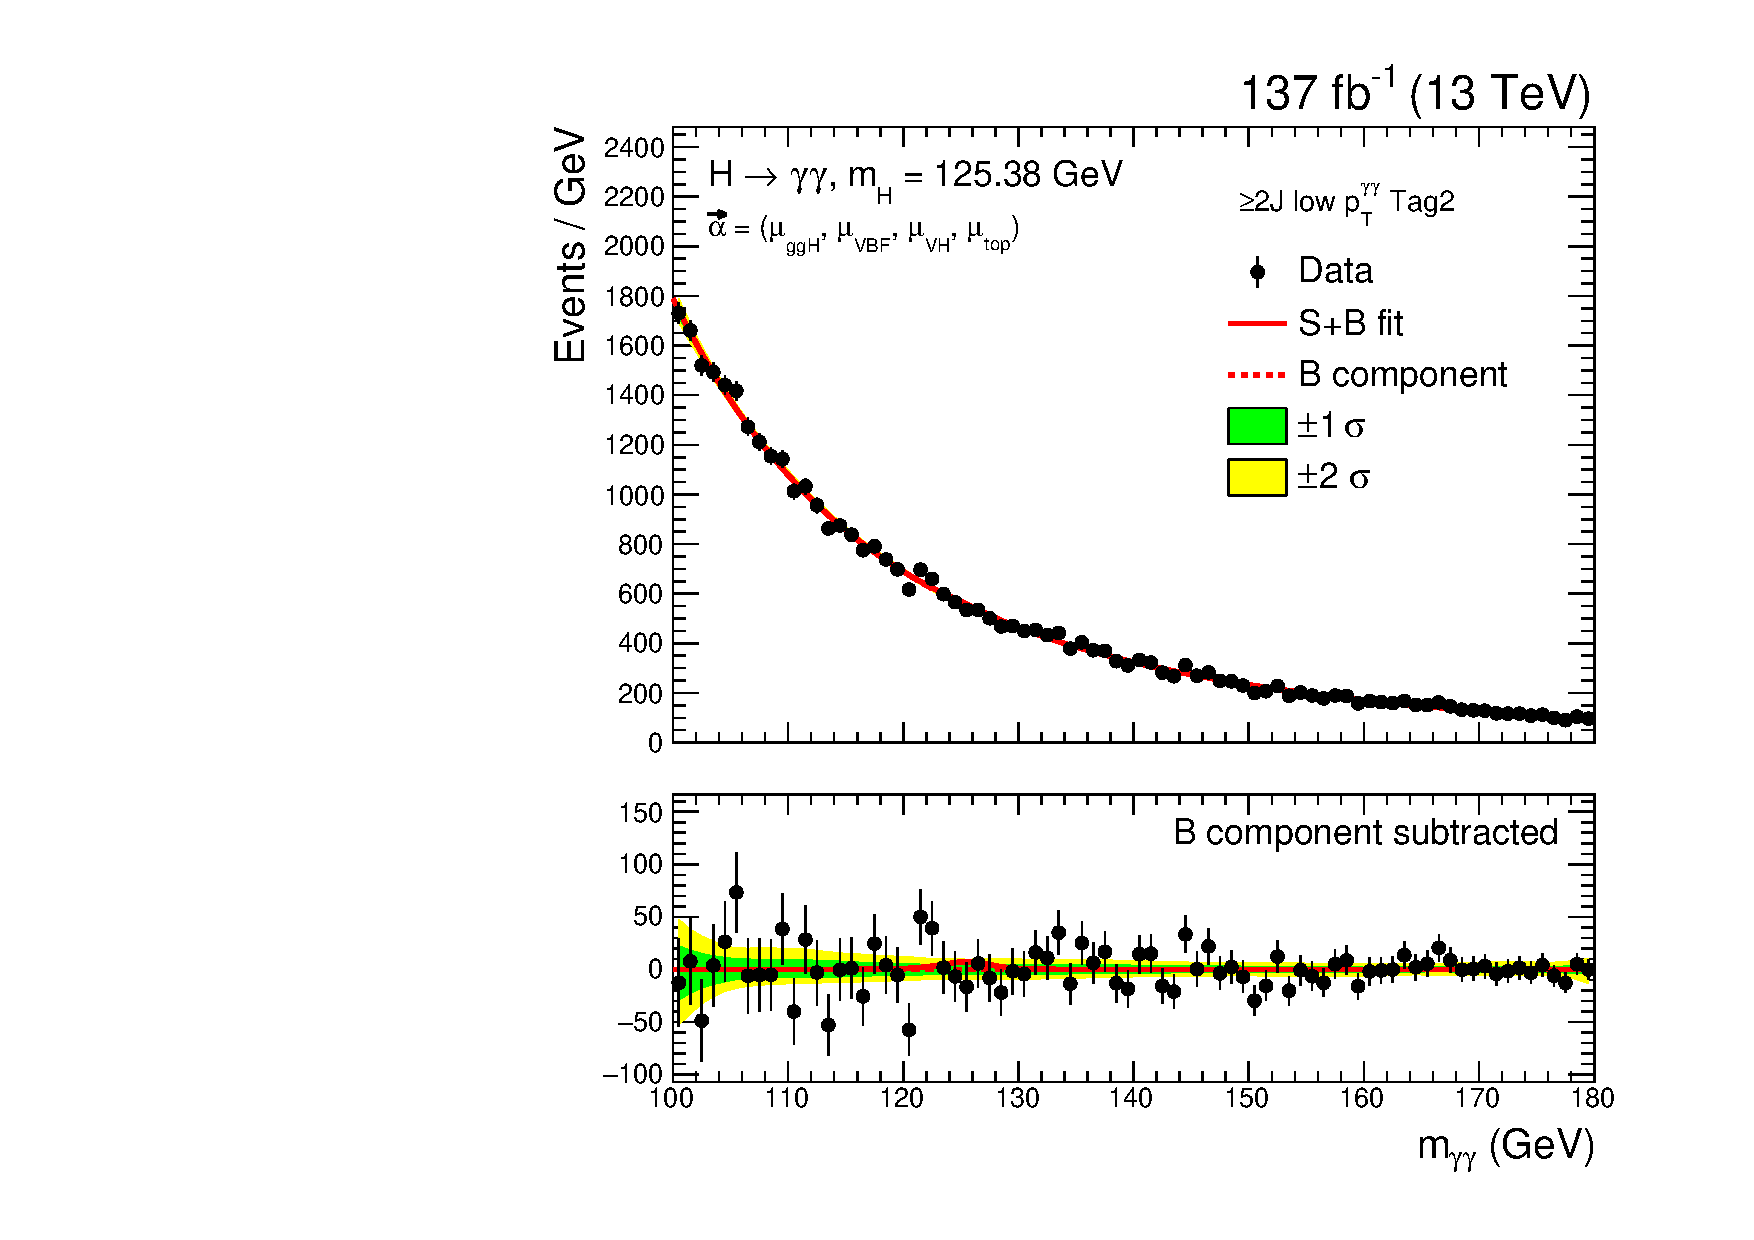
\includegraphics[width=.32\linewidth]{Figures/app_sb_models/RECO_GE2J_PTH_0_60_Tag2_CMS_hgg_mass.pdf}
  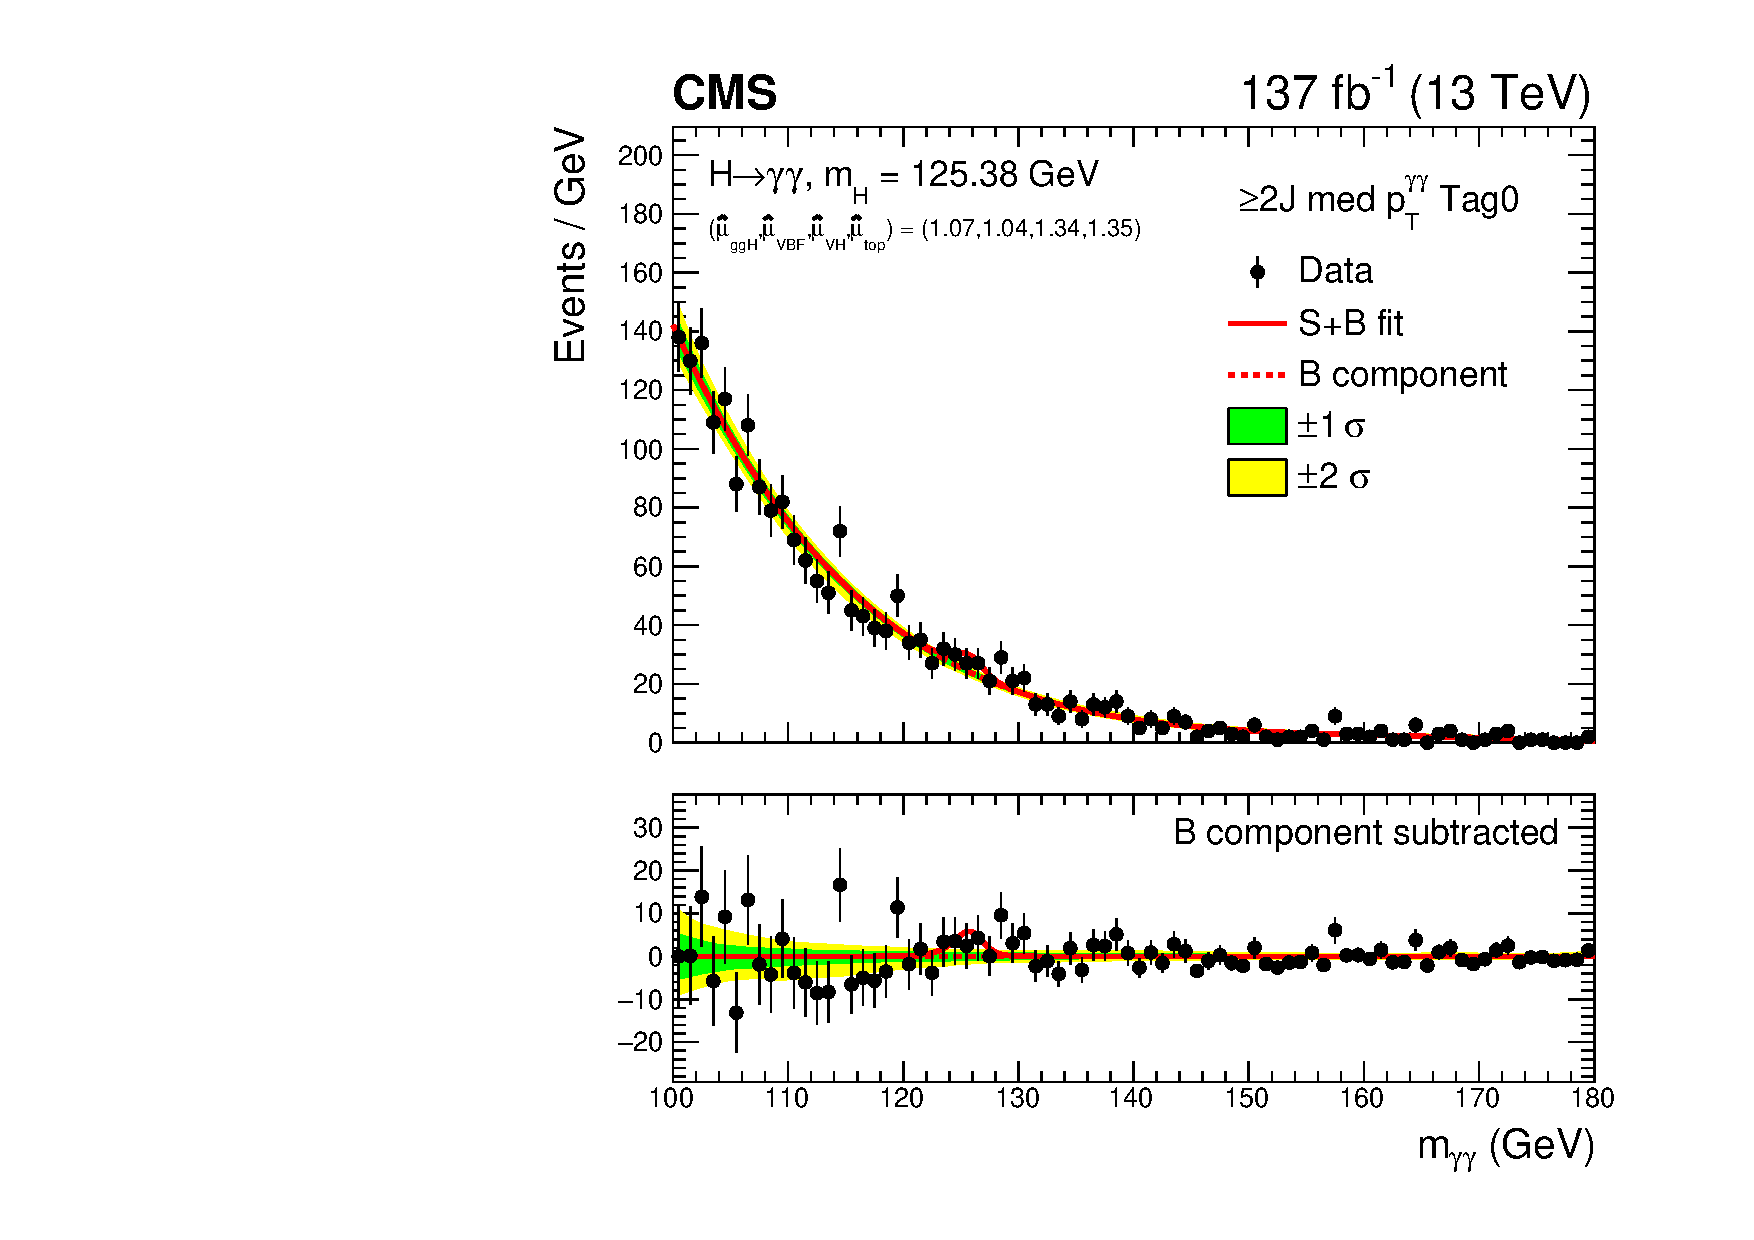
\includegraphics[width=.32\linewidth]{Figures/app_sb_models/RECO_GE2J_PTH_60_120_Tag0_CMS_hgg_mass.pdf}
  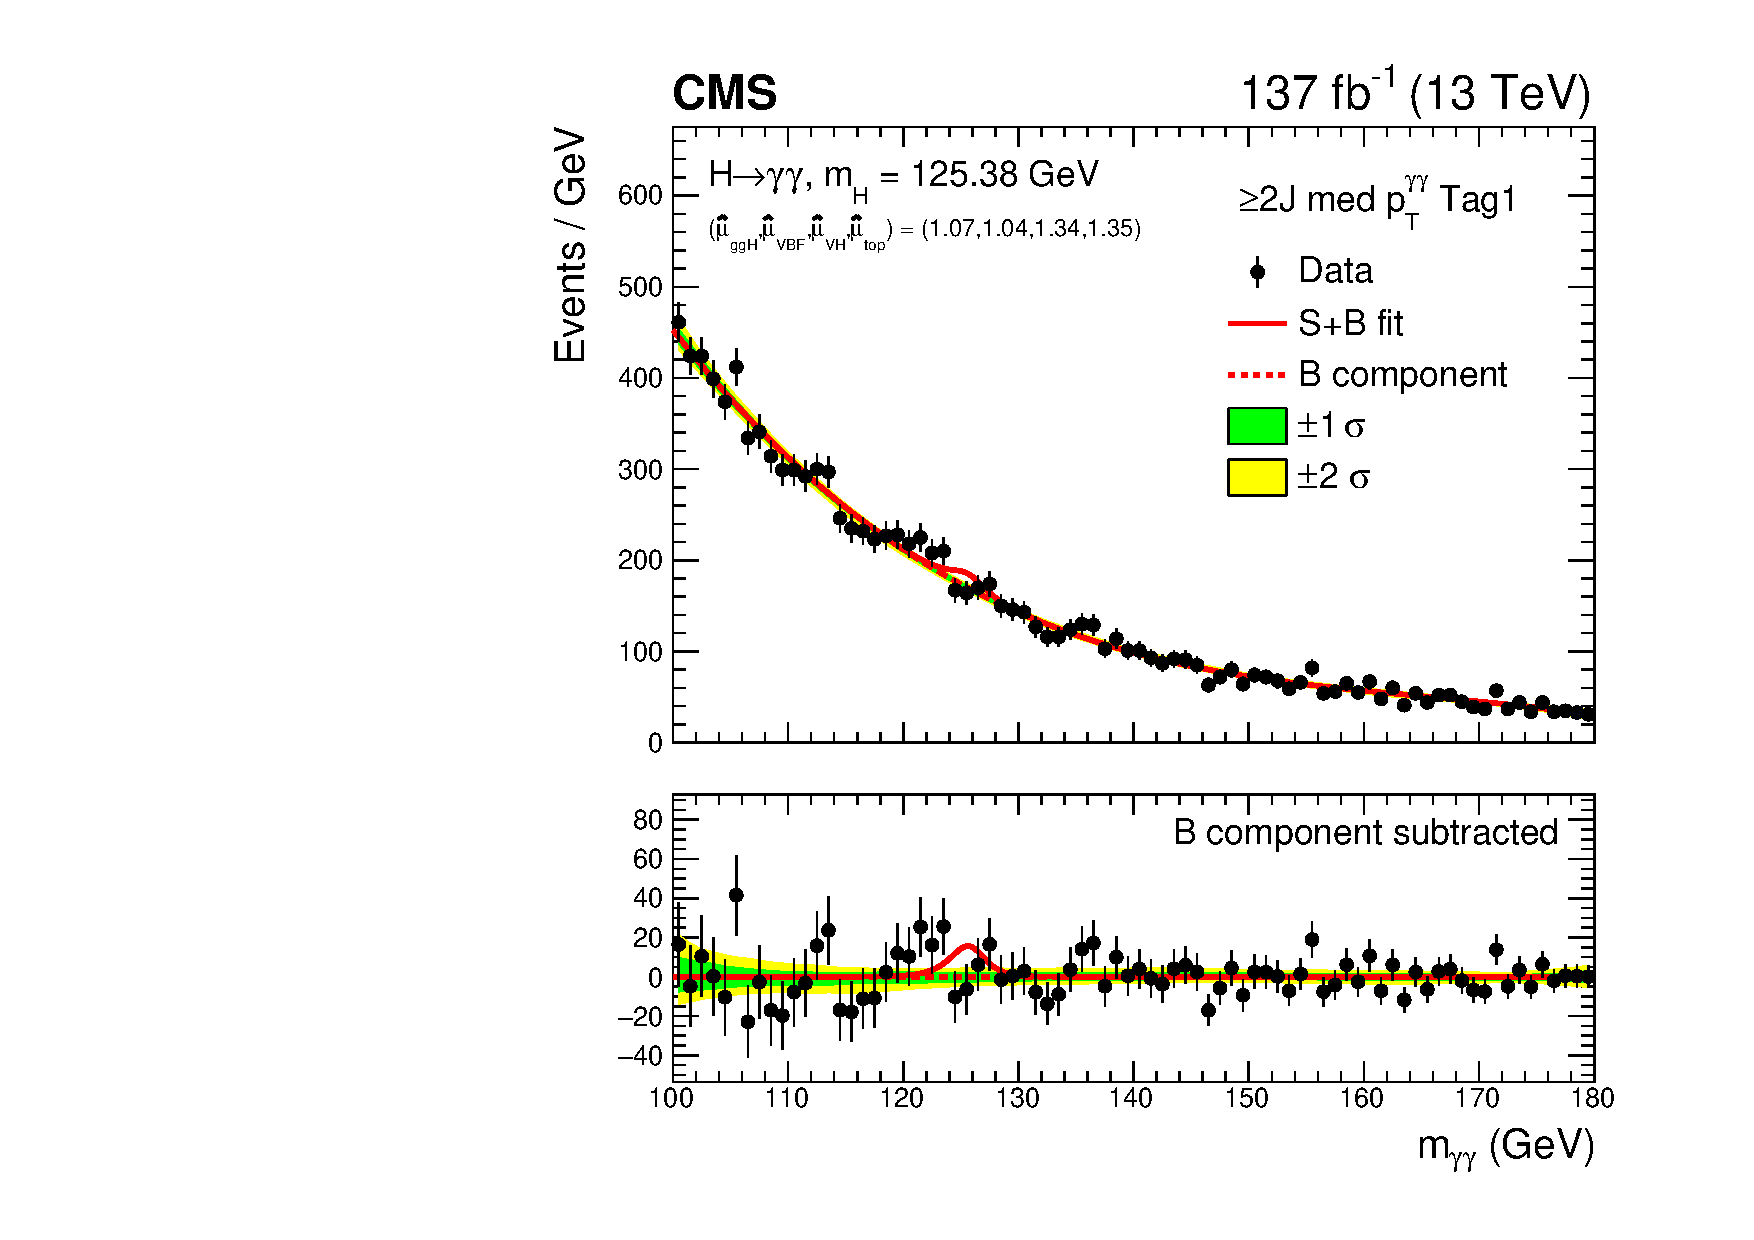
\includegraphics[width=.32\linewidth]{Figures/app_sb_models/RECO_GE2J_PTH_60_120_Tag1_CMS_hgg_mass.pdf}
  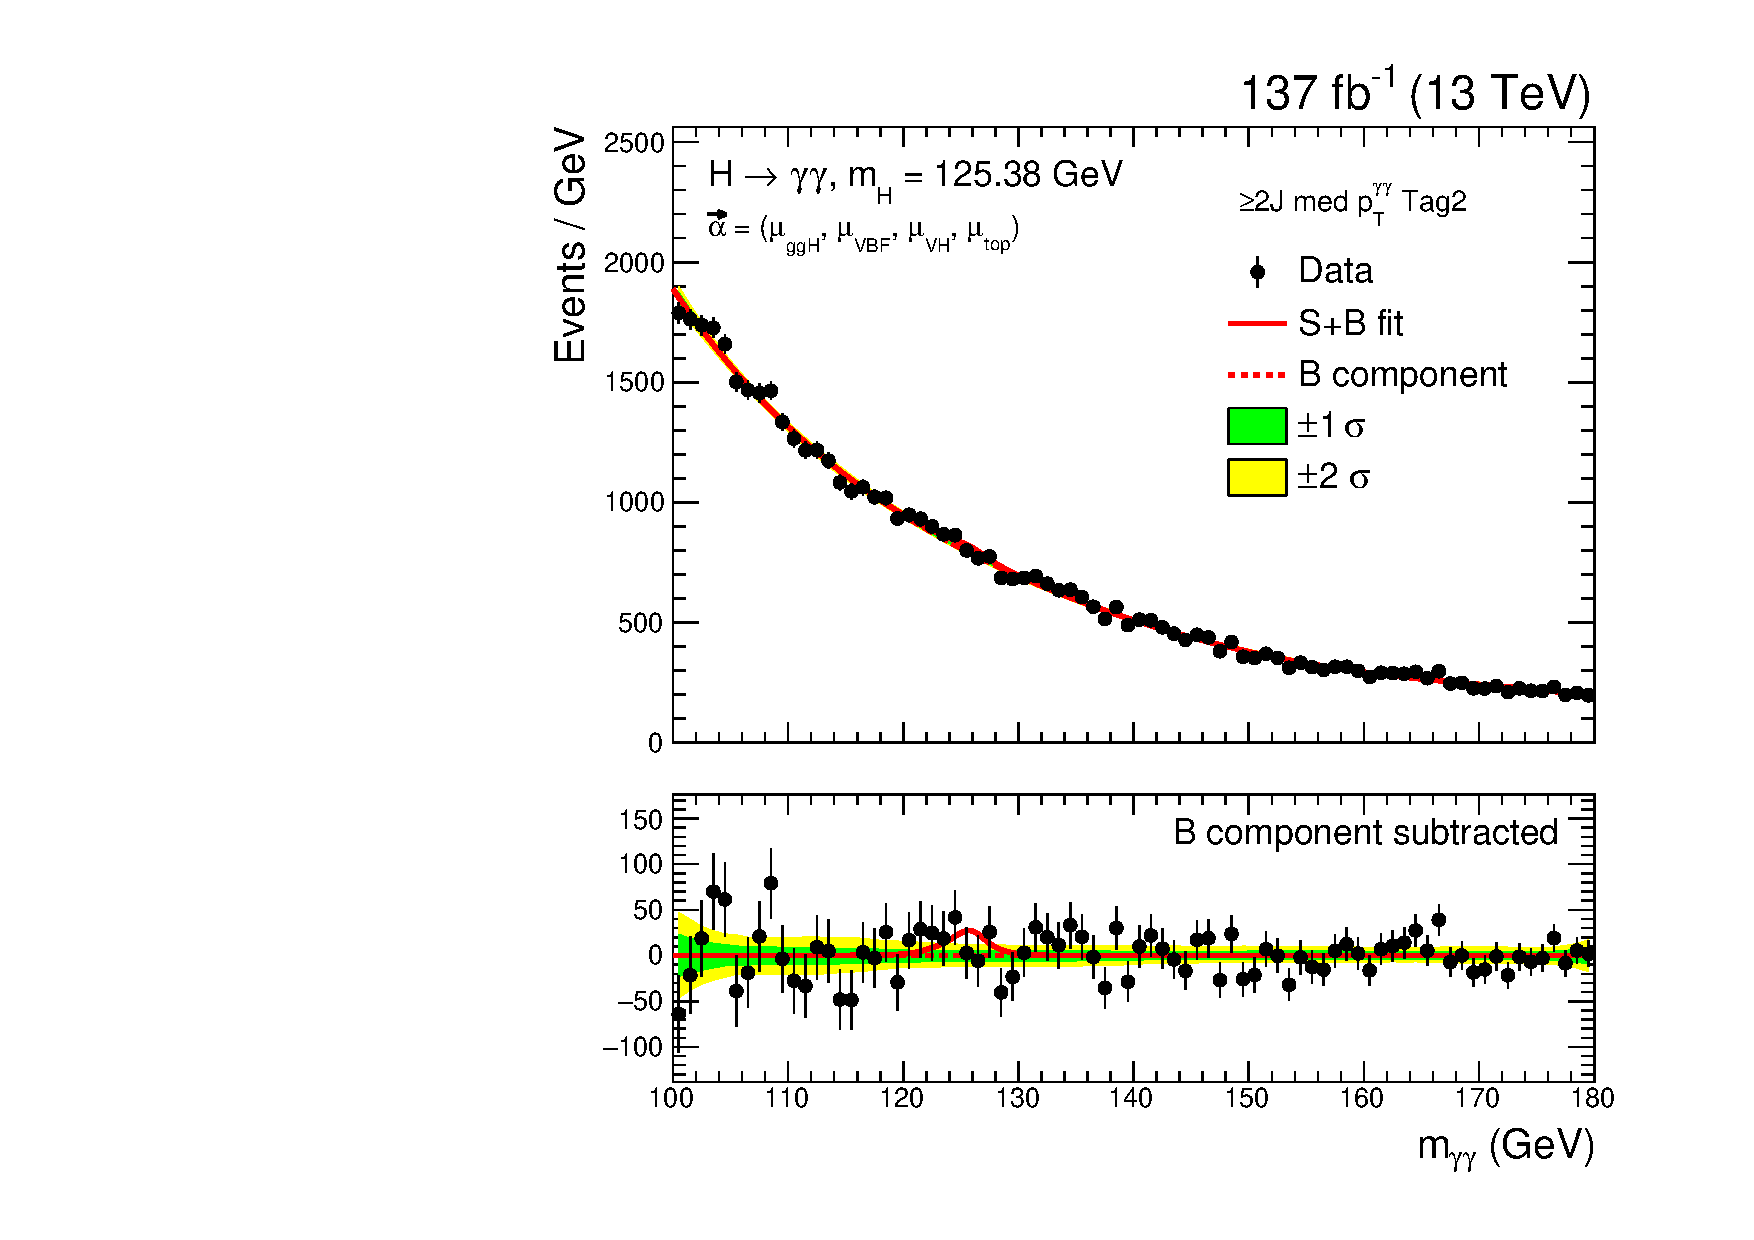
\includegraphics[width=.32\linewidth]{Figures/app_sb_models/RECO_GE2J_PTH_60_120_Tag2_CMS_hgg_mass.pdf}
  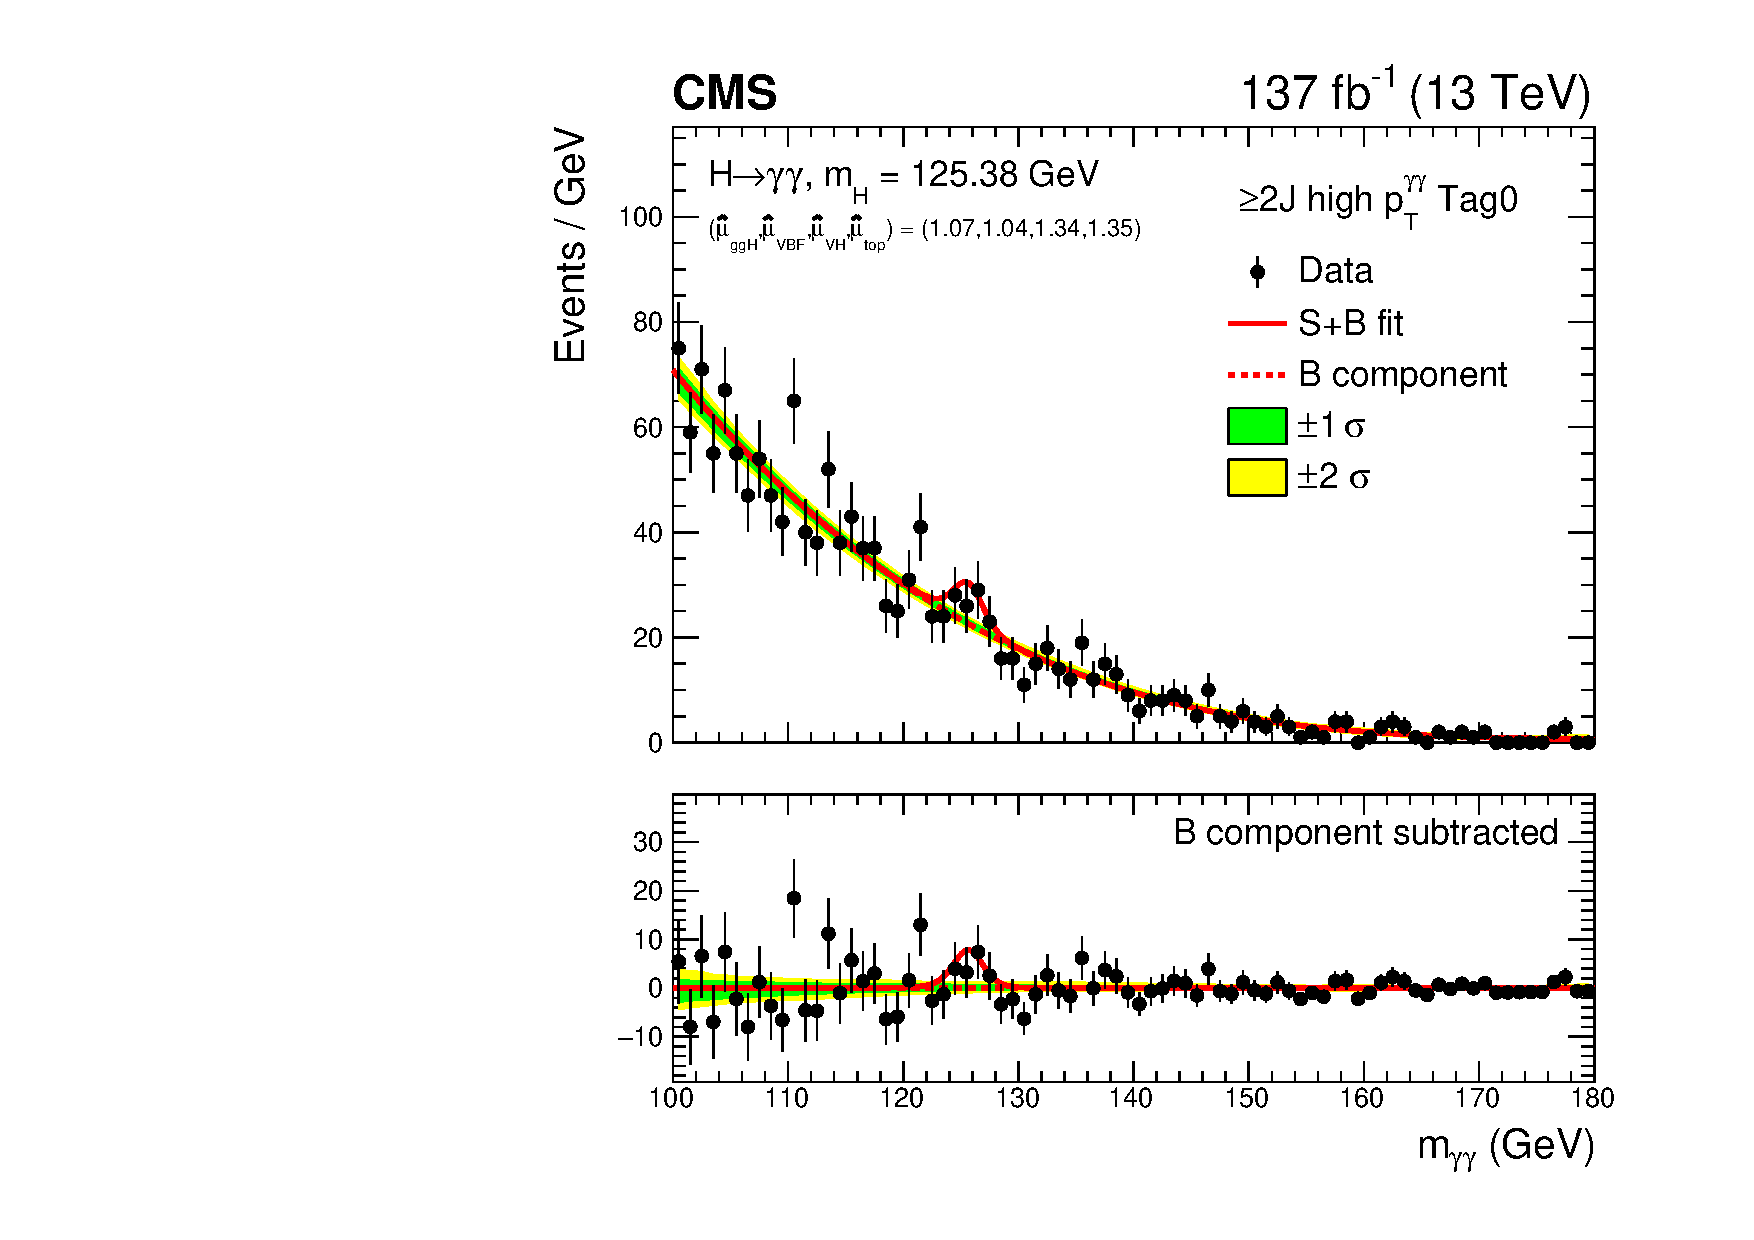
\includegraphics[width=.32\linewidth]{Figures/app_sb_models/RECO_GE2J_PTH_120_200_Tag0_CMS_hgg_mass.pdf}
  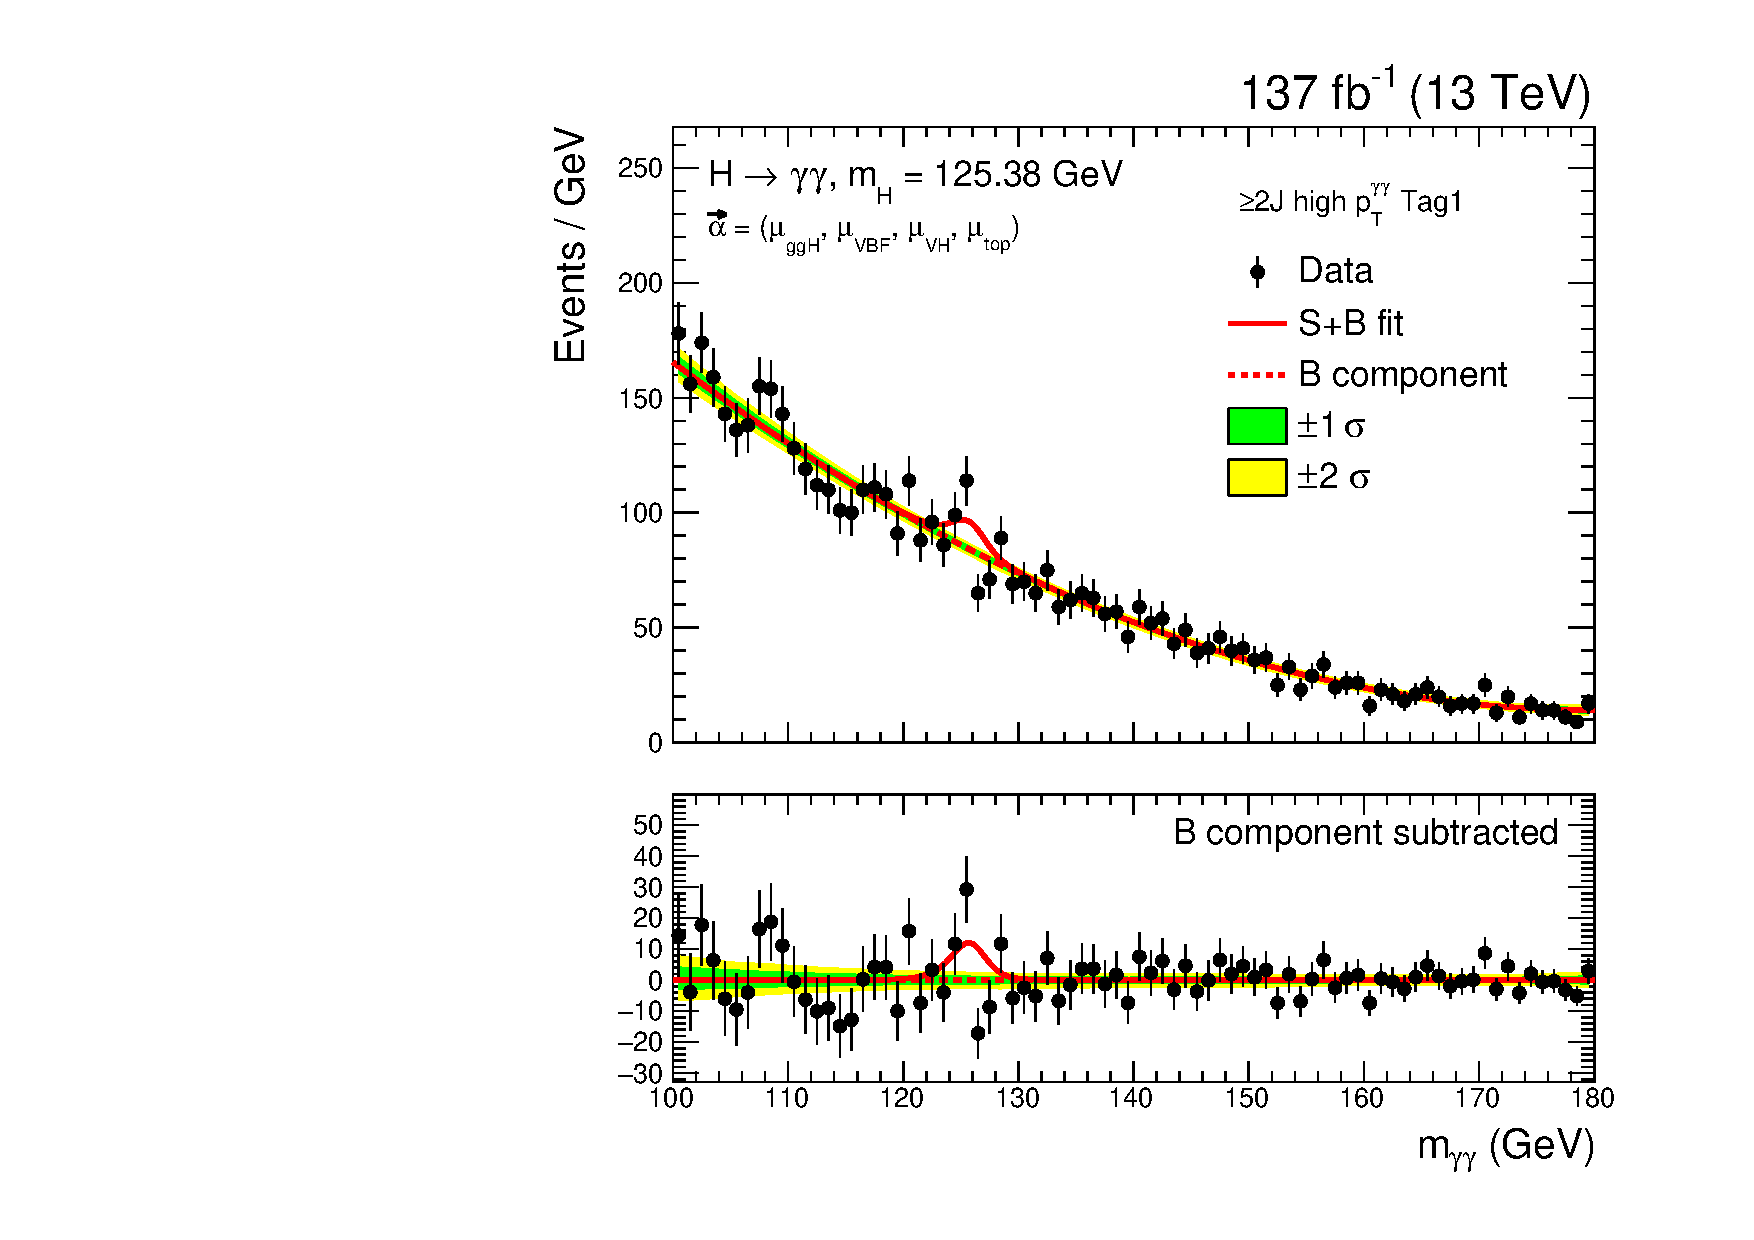
\includegraphics[width=.32\linewidth]{Figures/app_sb_models/RECO_GE2J_PTH_120_200_Tag1_CMS_hgg_mass.pdf}
  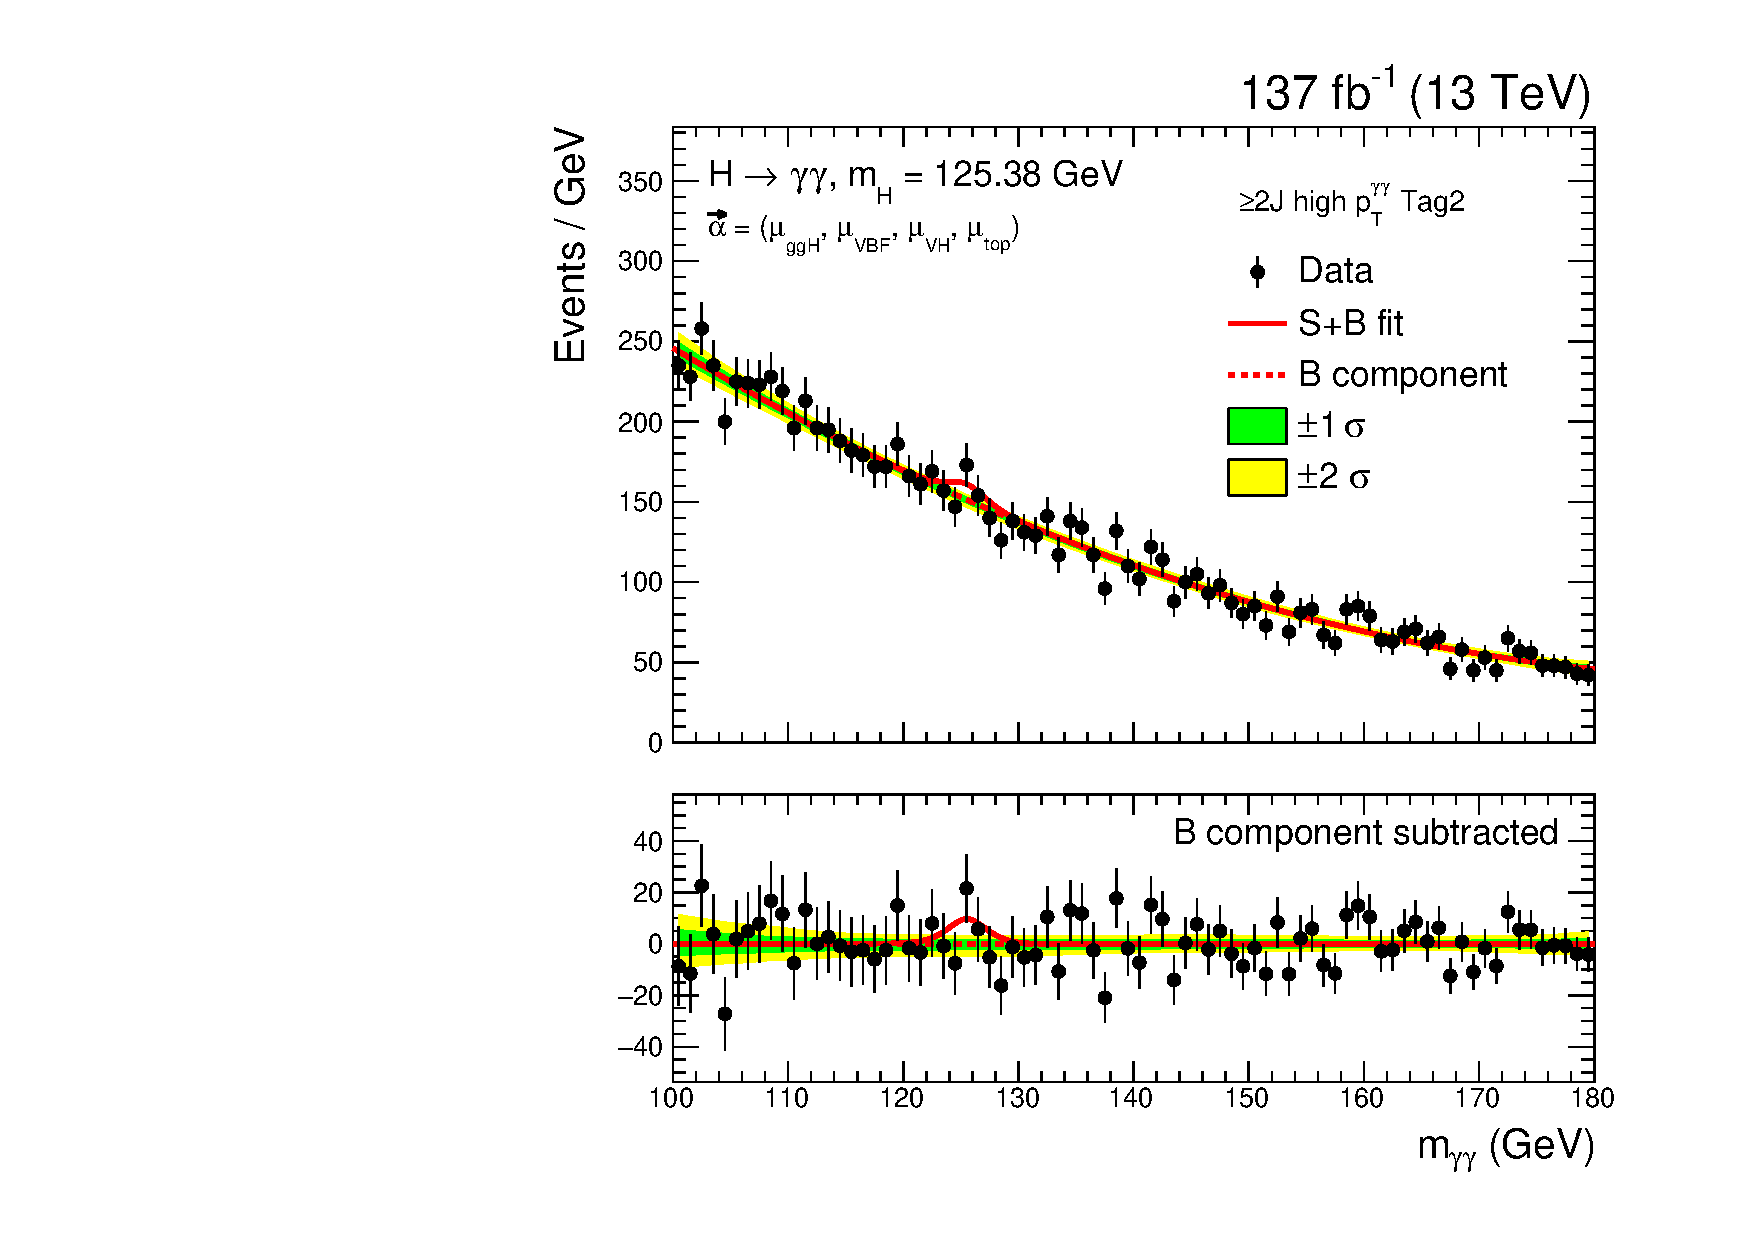
\includegraphics[width=.32\linewidth]{Figures/app_sb_models/RECO_GE2J_PTH_120_200_Tag2_CMS_hgg_mass.pdf}
  \caption[Observed diphoton mass distributions: ggH 1J and ggH $\geq$2J]
  {
    Data points (black) and the best-fit signal-plus-background model for the individual analysis categories targeting a number of ggH STXS regions. The best-fit model corresponds to the per-production mode signal strength fit. The solid red line shows the best-fit signal-plus-background model, whereas the dashed line shows the background component only. The one standard deviation (green) and two standard deviation (yellow) bands show the uncertainties in the background component of the fit. The bottom panels in each plot show the residuals after subtraction of this background component.
  }
  \label{fig:diphoton_mass_1}
\end{figure}


\begin{figure}[htbp]
  \centering
  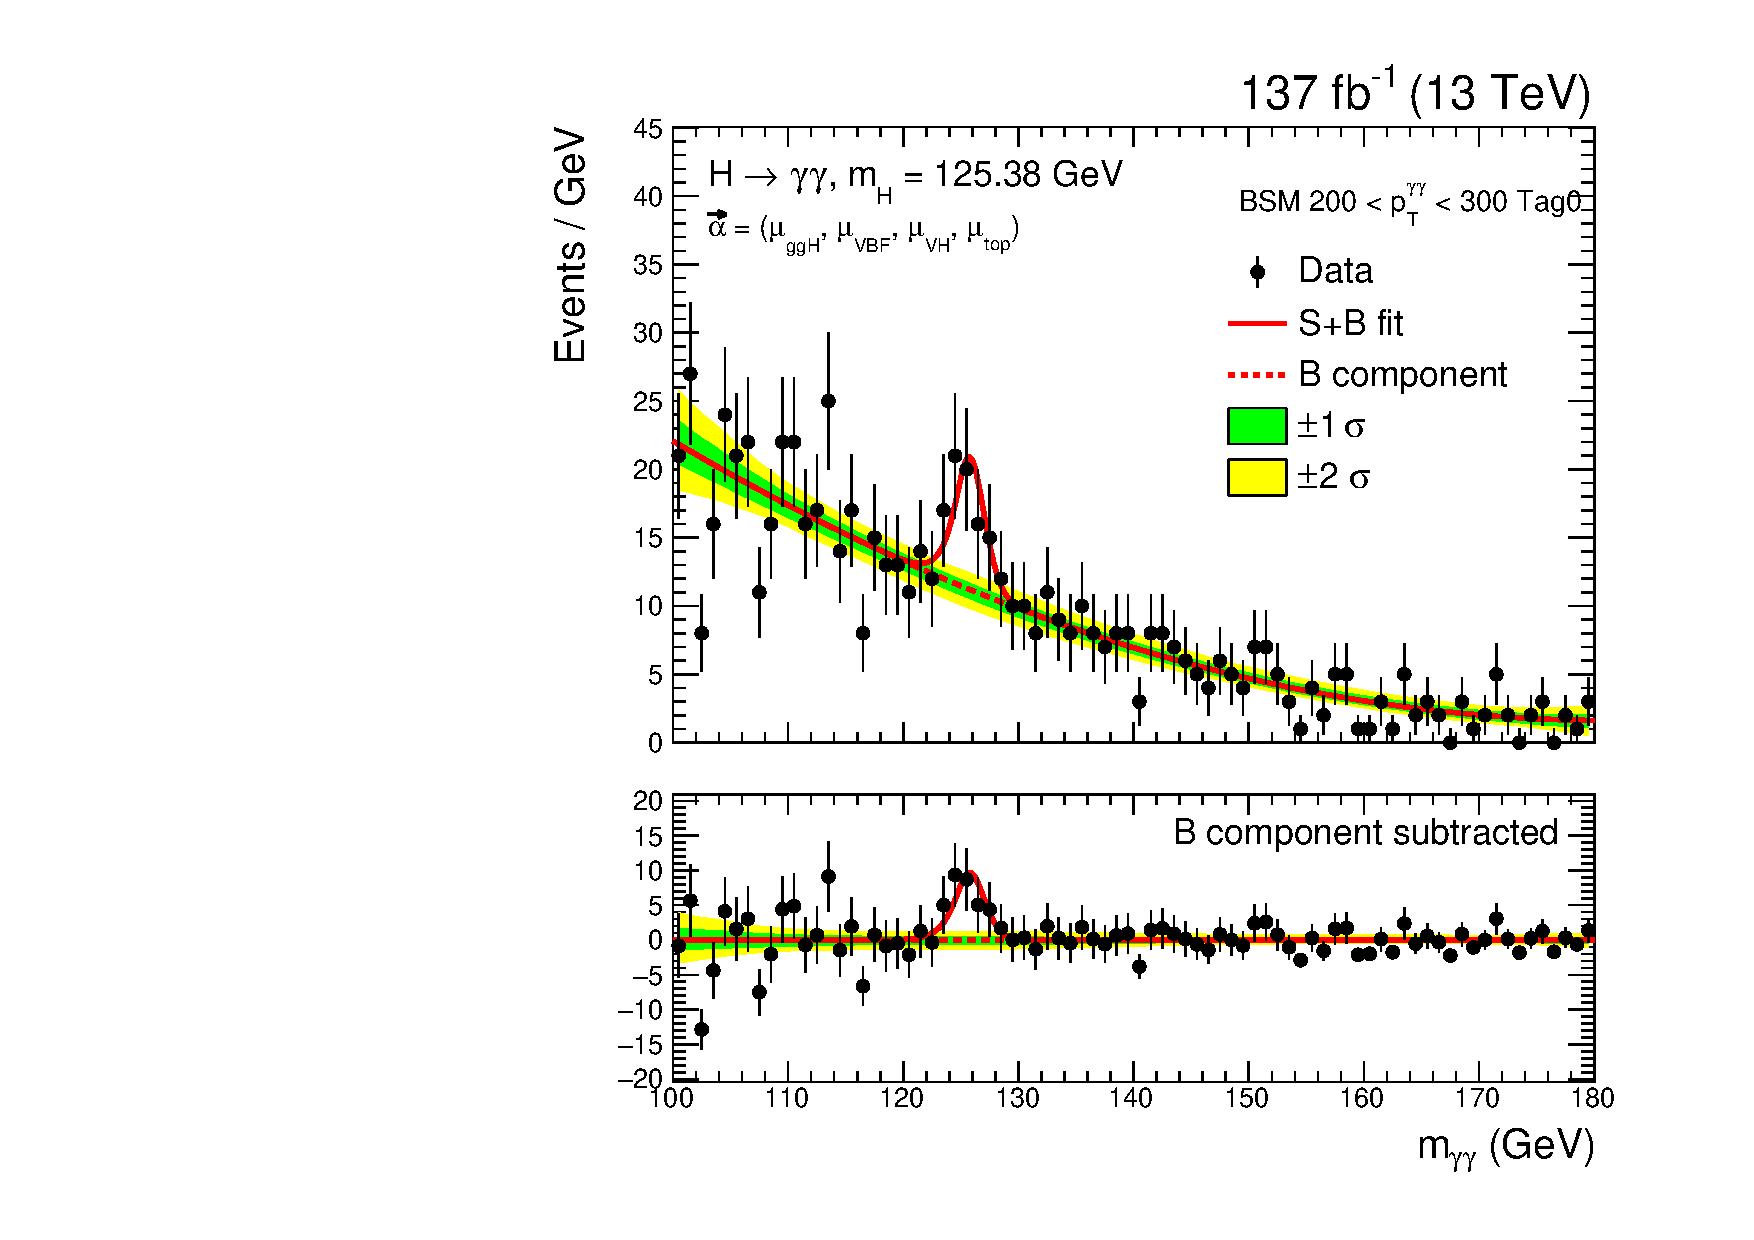
\includegraphics[width=.32\linewidth]{Figures/app_sb_models/RECO_PTH_200_300_Tag0_CMS_hgg_mass.pdf}
  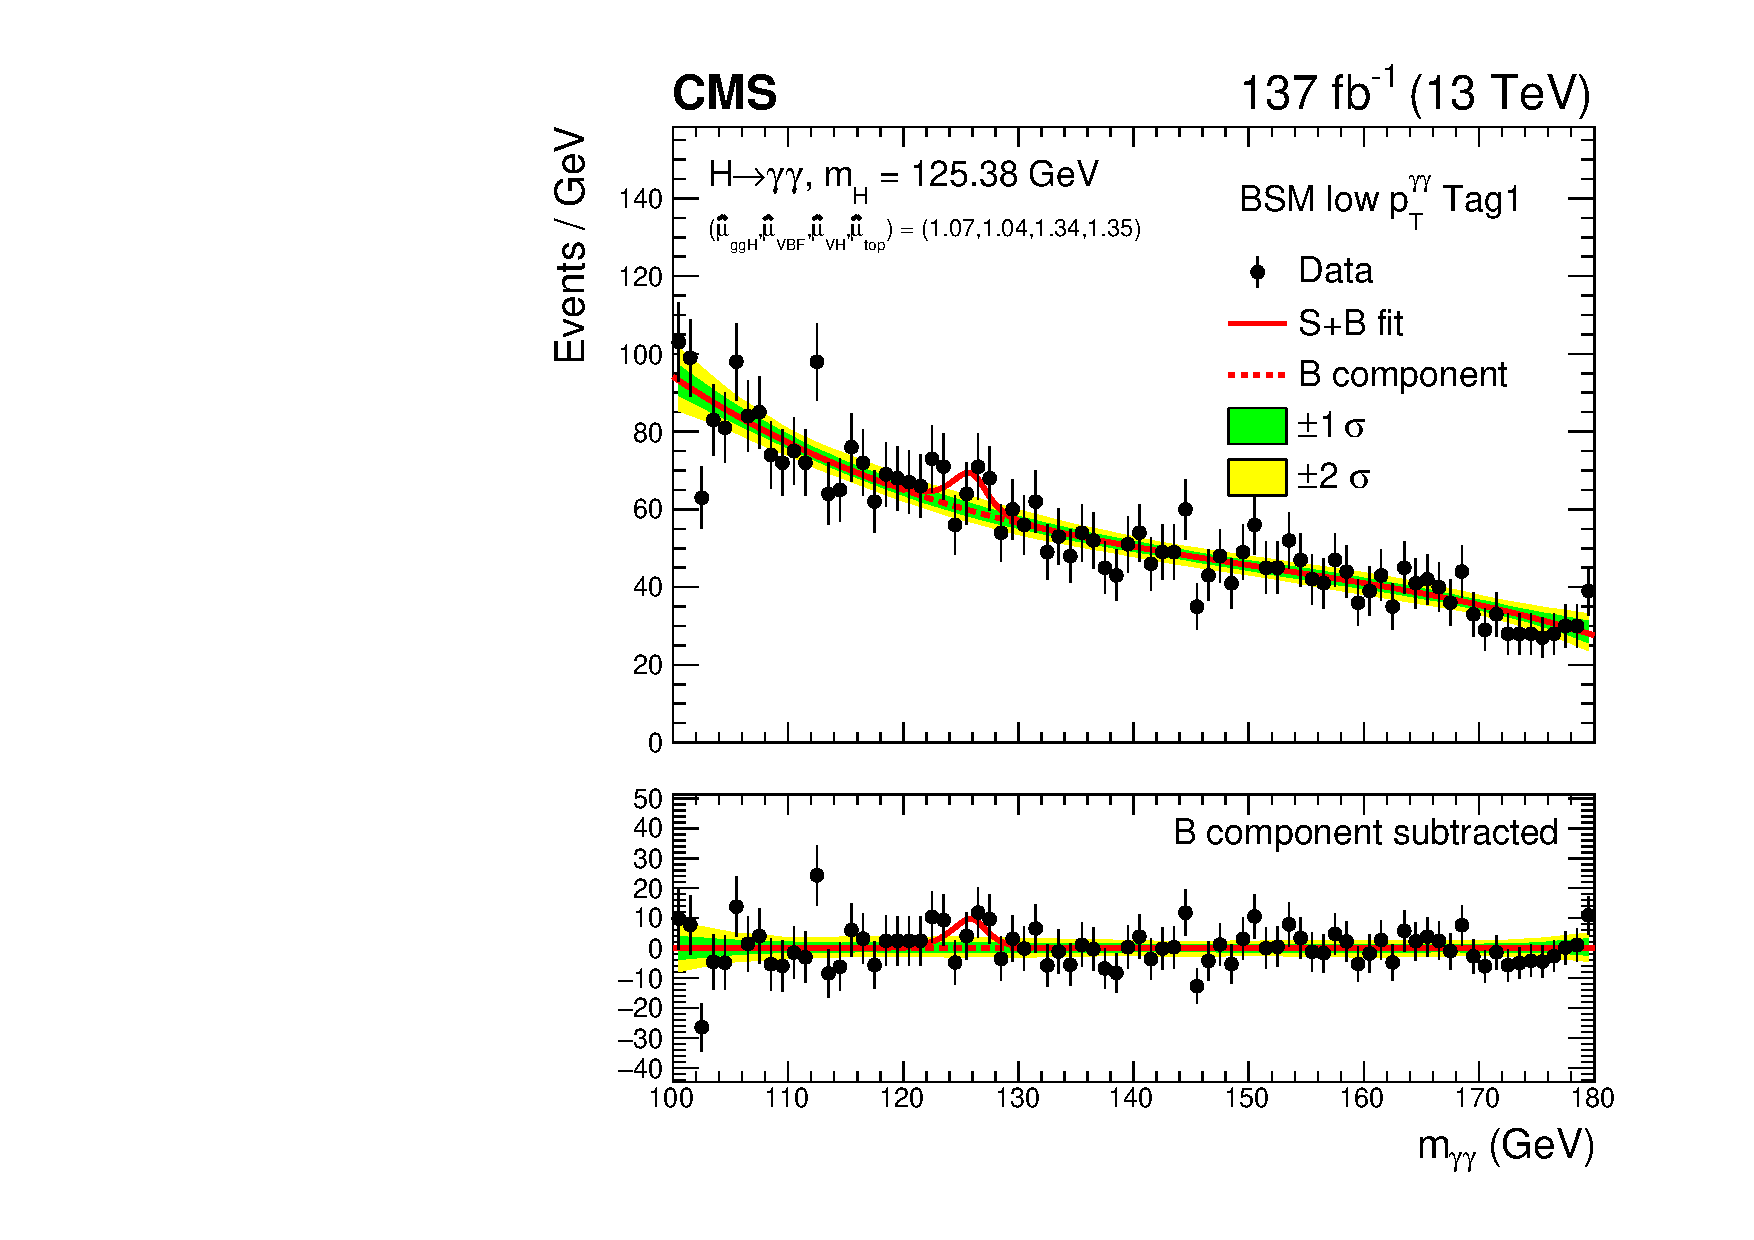
\includegraphics[width=.32\linewidth]{Figures/app_sb_models/RECO_PTH_200_300_Tag1_CMS_hgg_mass.pdf}
  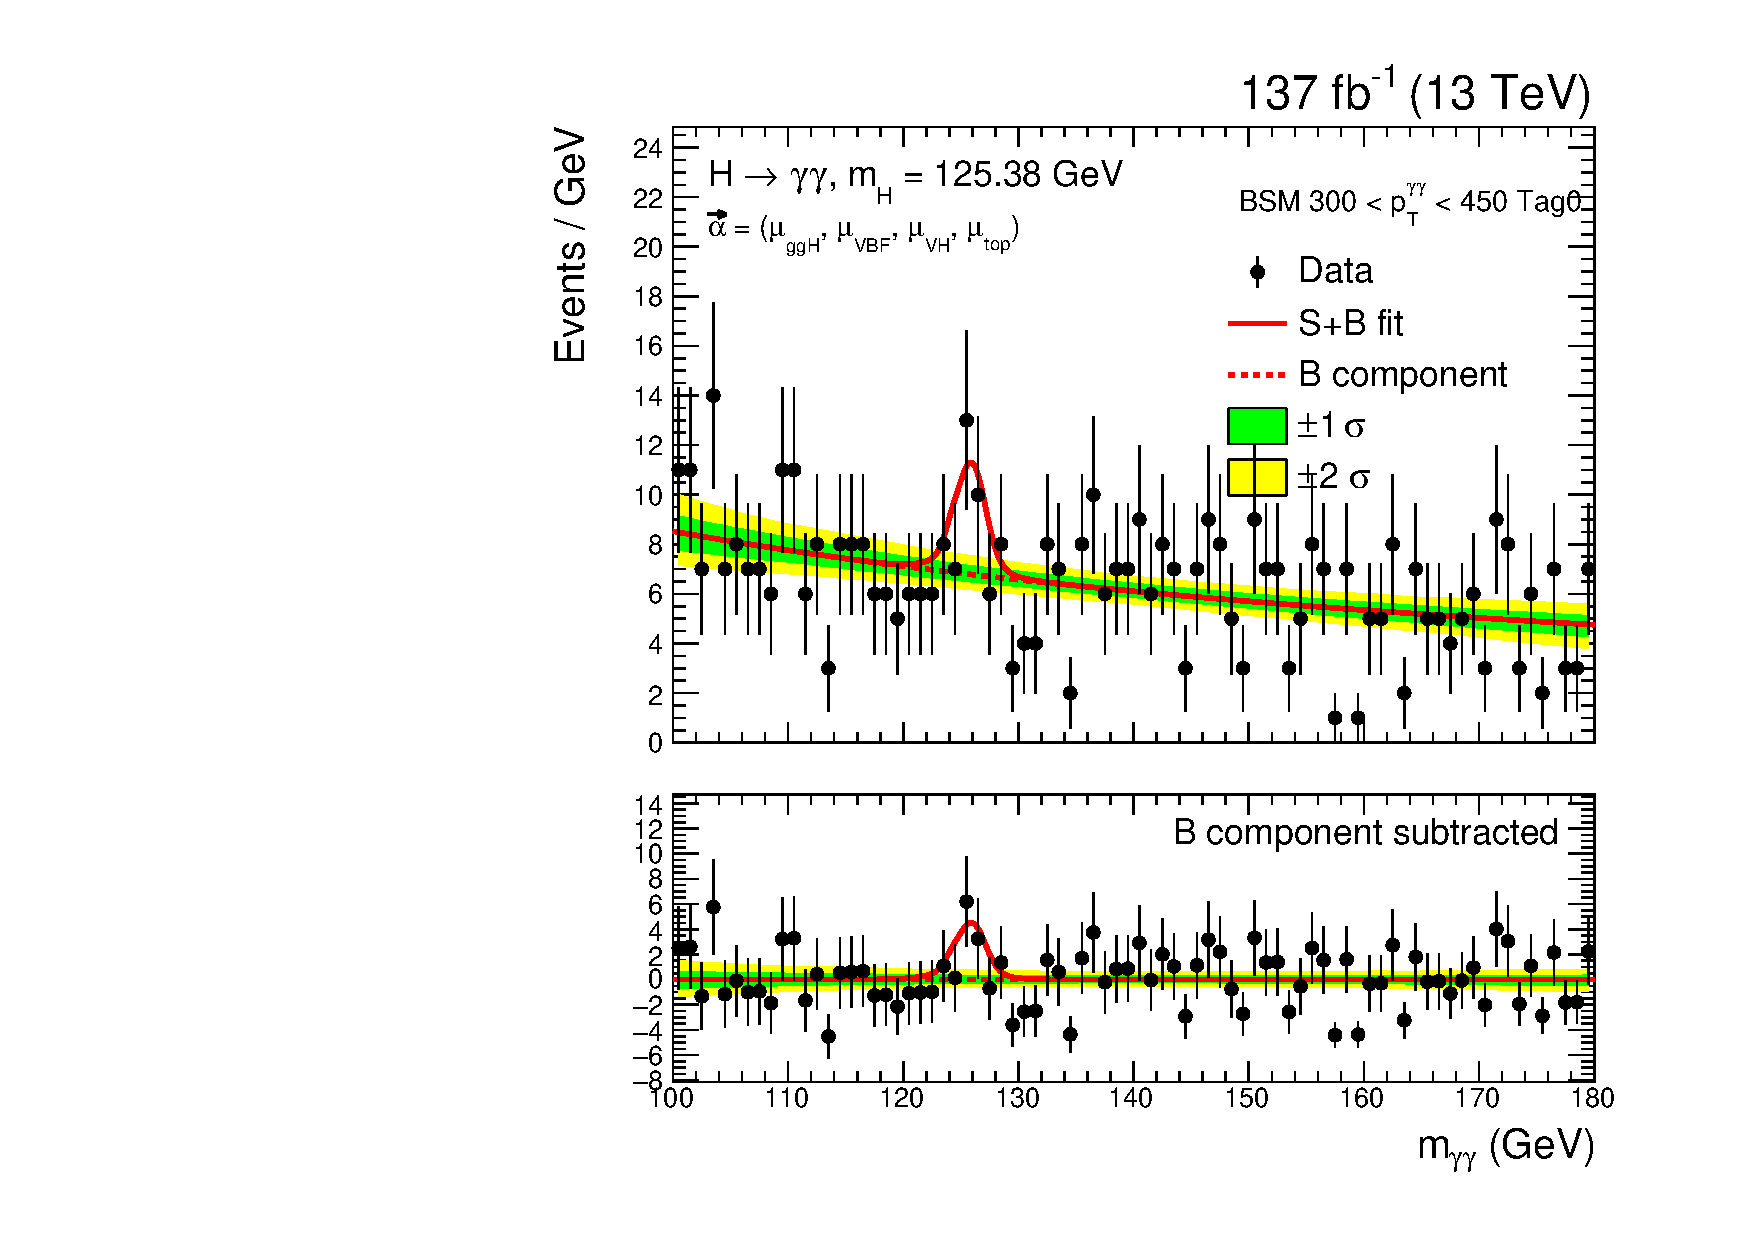
\includegraphics[width=.32\linewidth]{Figures/app_sb_models/RECO_PTH_300_450_Tag0_CMS_hgg_mass.pdf}
  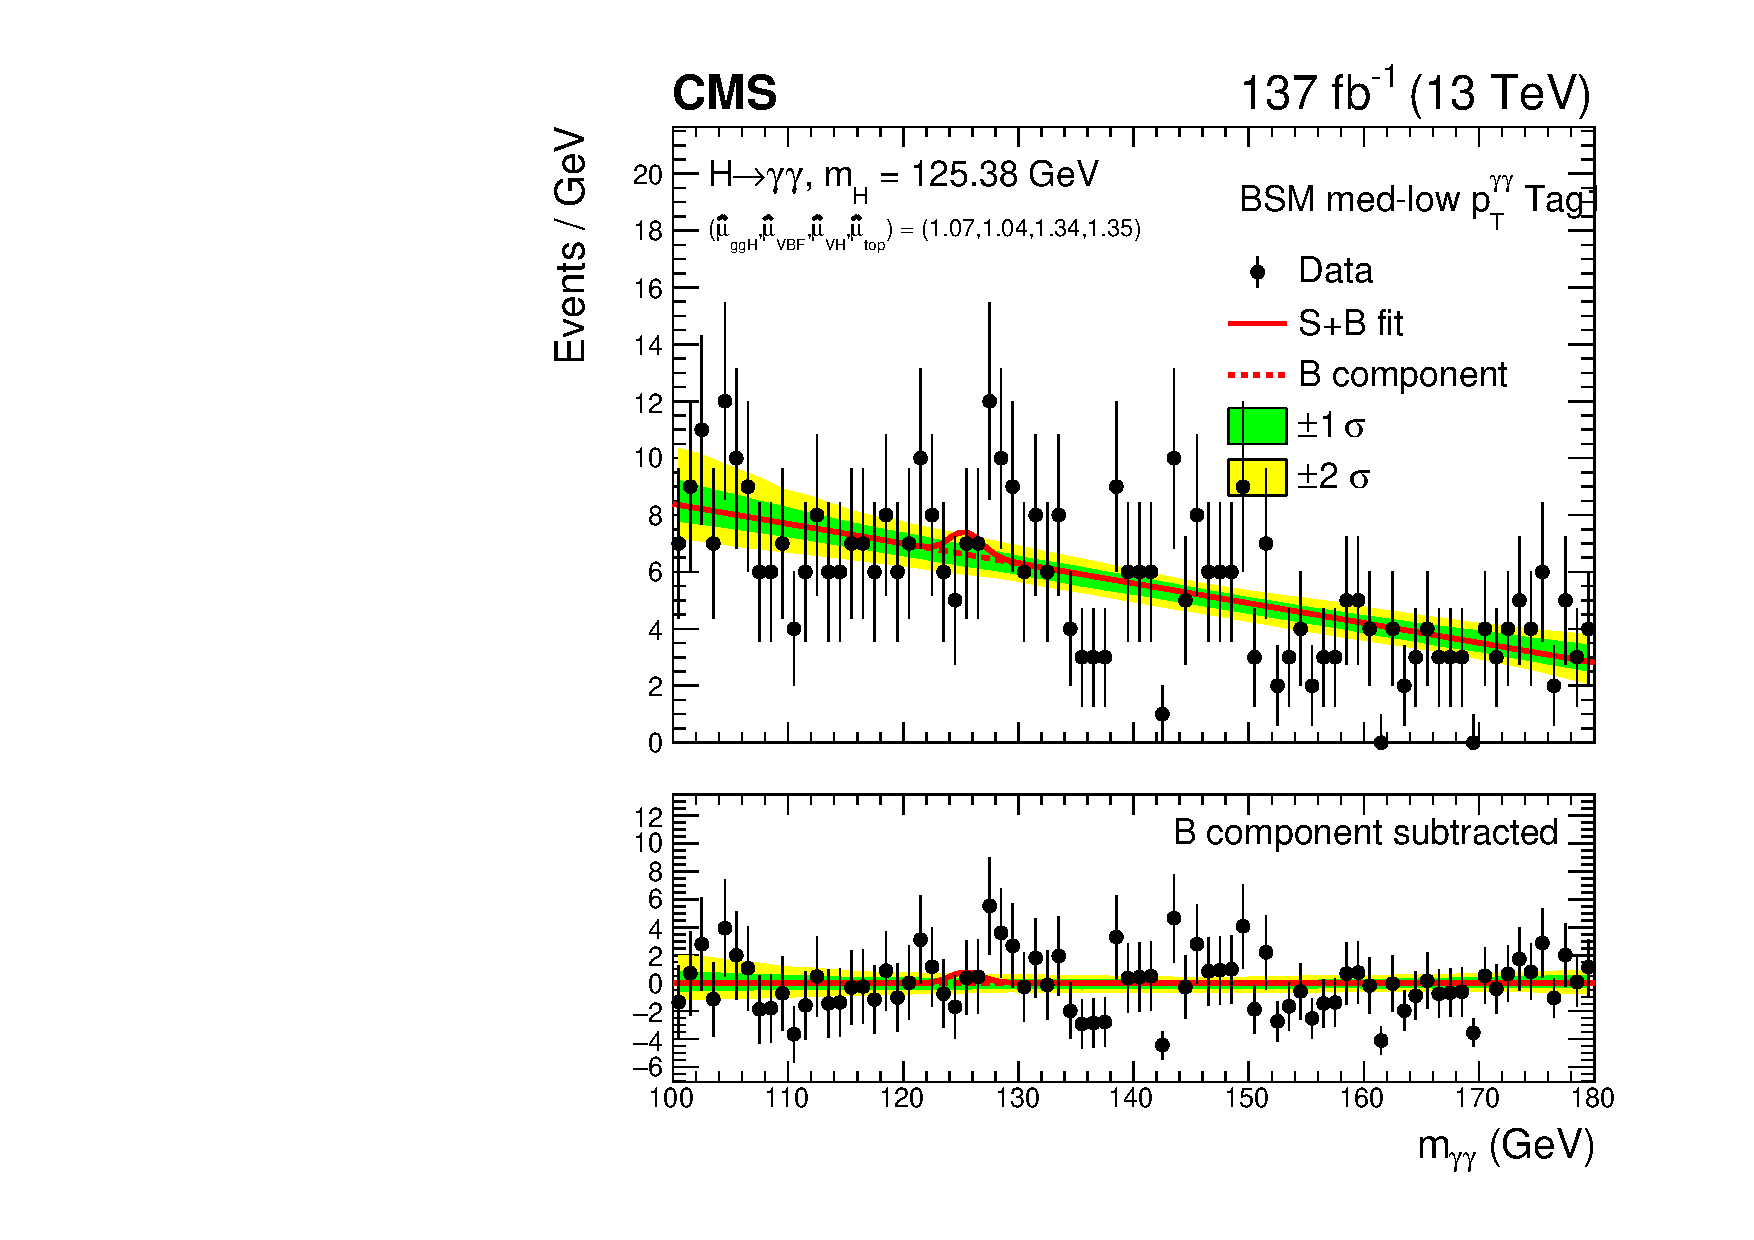
\includegraphics[width=.32\linewidth]{Figures/app_sb_models/RECO_PTH_300_450_Tag1_CMS_hgg_mass.pdf}
  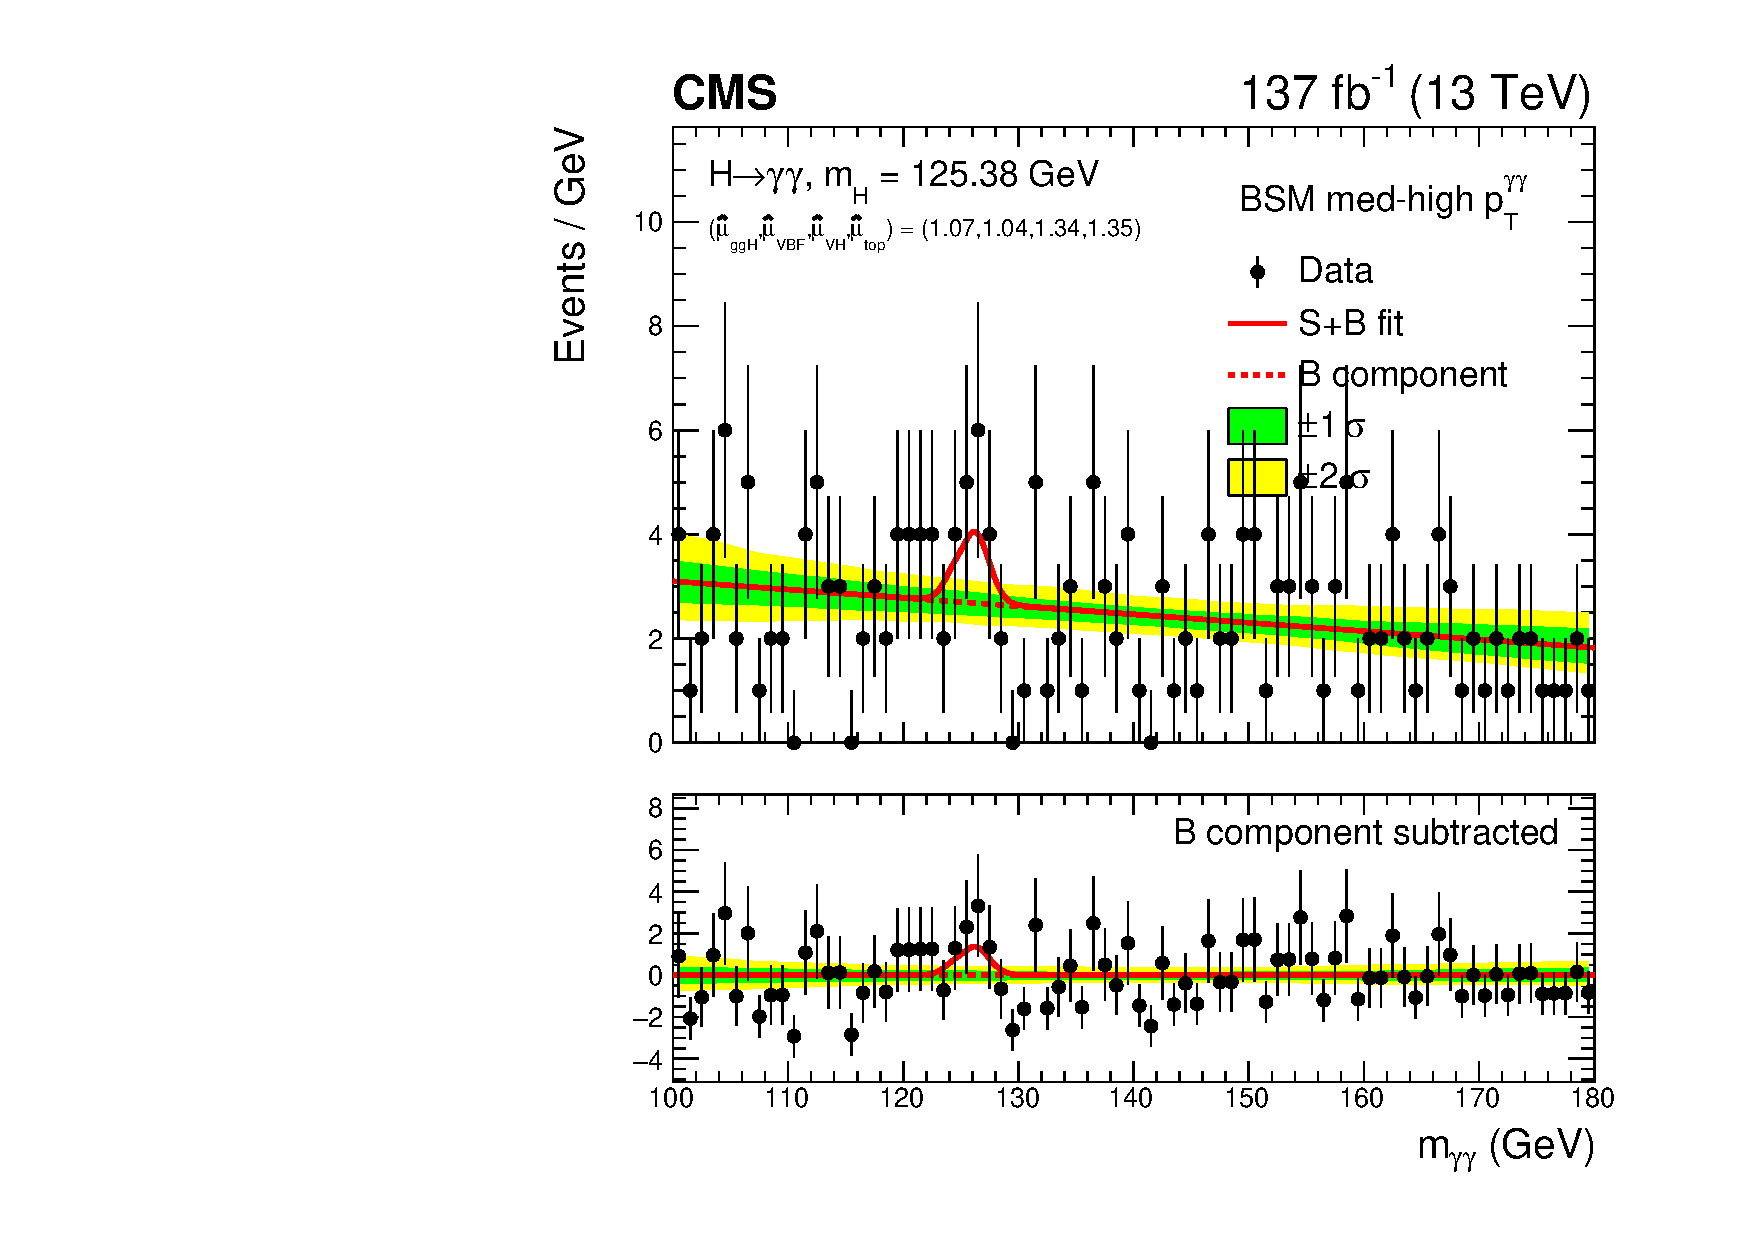
\includegraphics[width=.32\linewidth]{Figures/app_sb_models/RECO_PTH_450_650_Tag0_CMS_hgg_mass.pdf}
  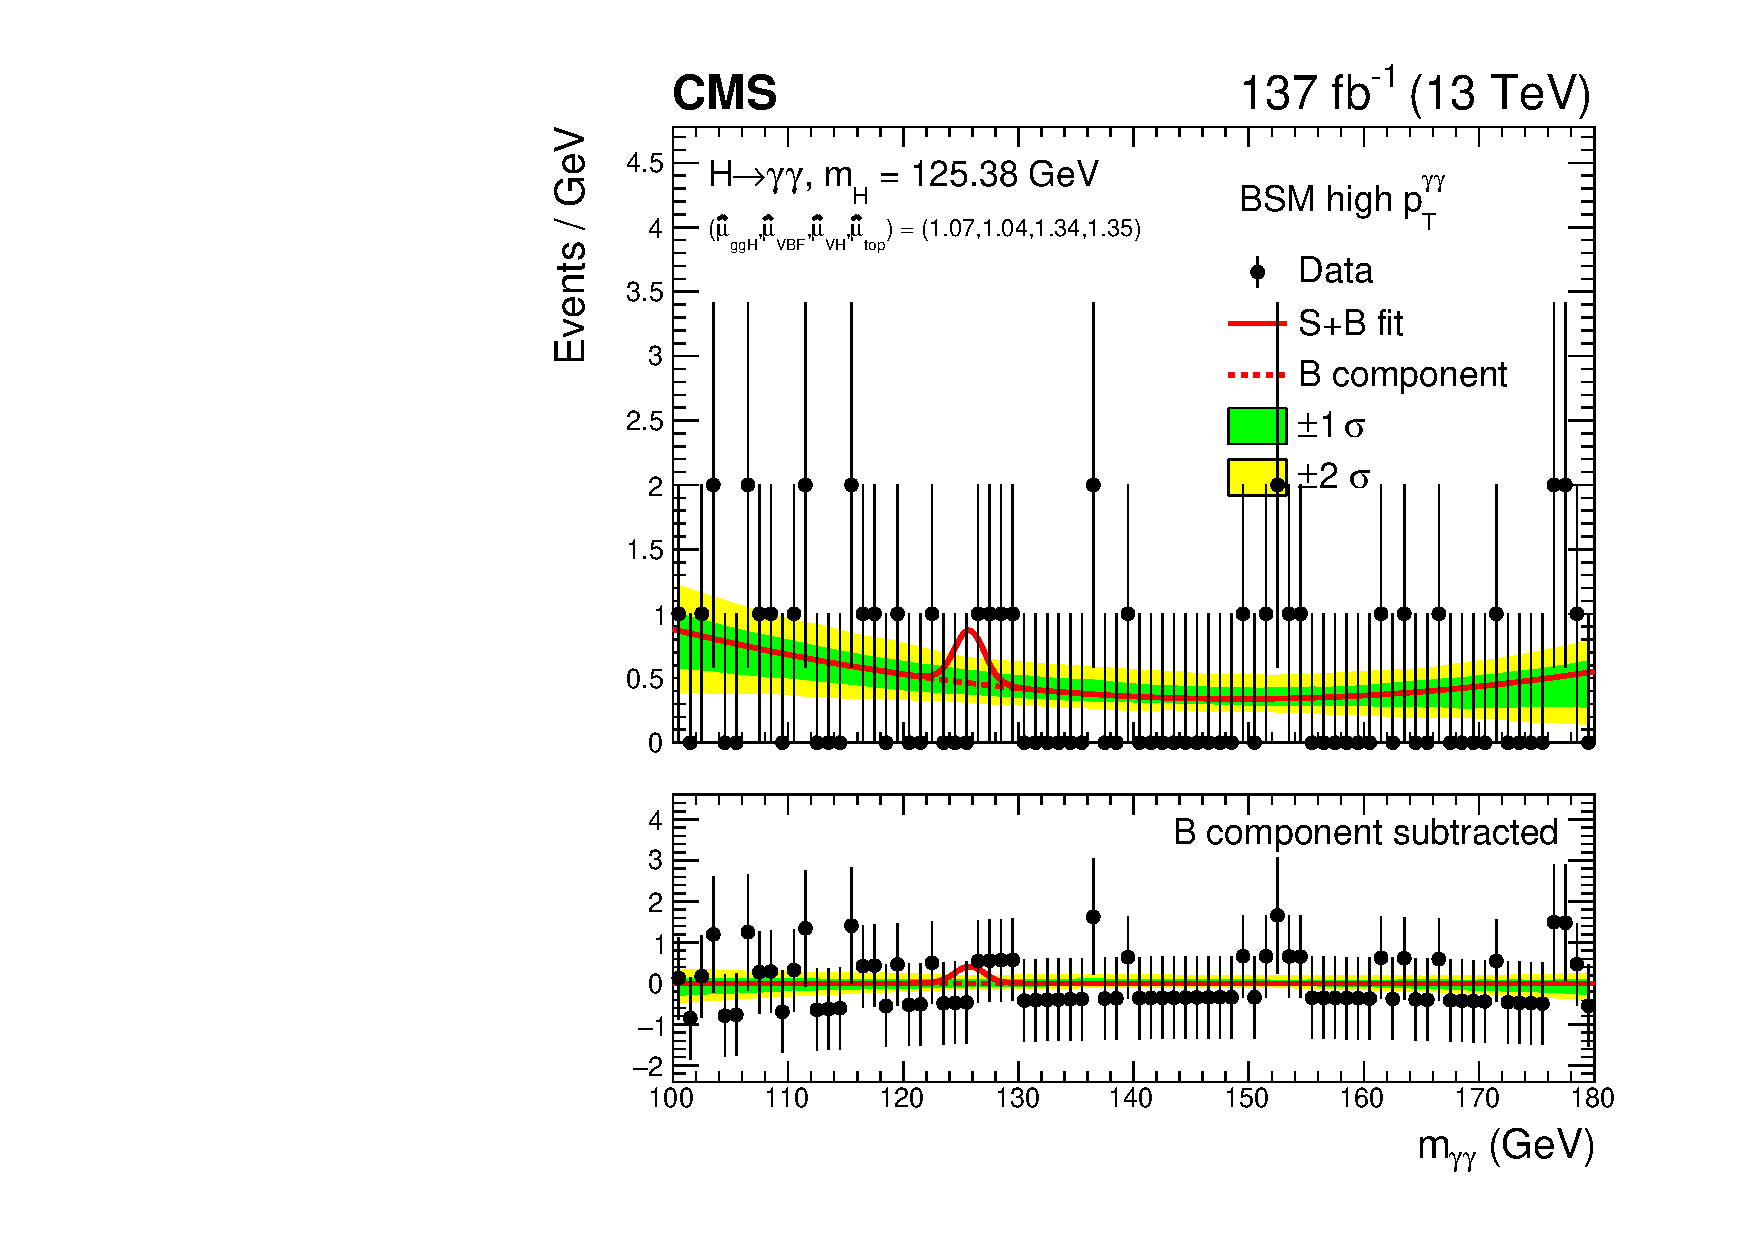
\includegraphics[width=.32\linewidth]{Figures/app_sb_models/RECO_PTH_GT650_Tag0_CMS_hgg_mass.pdf}
  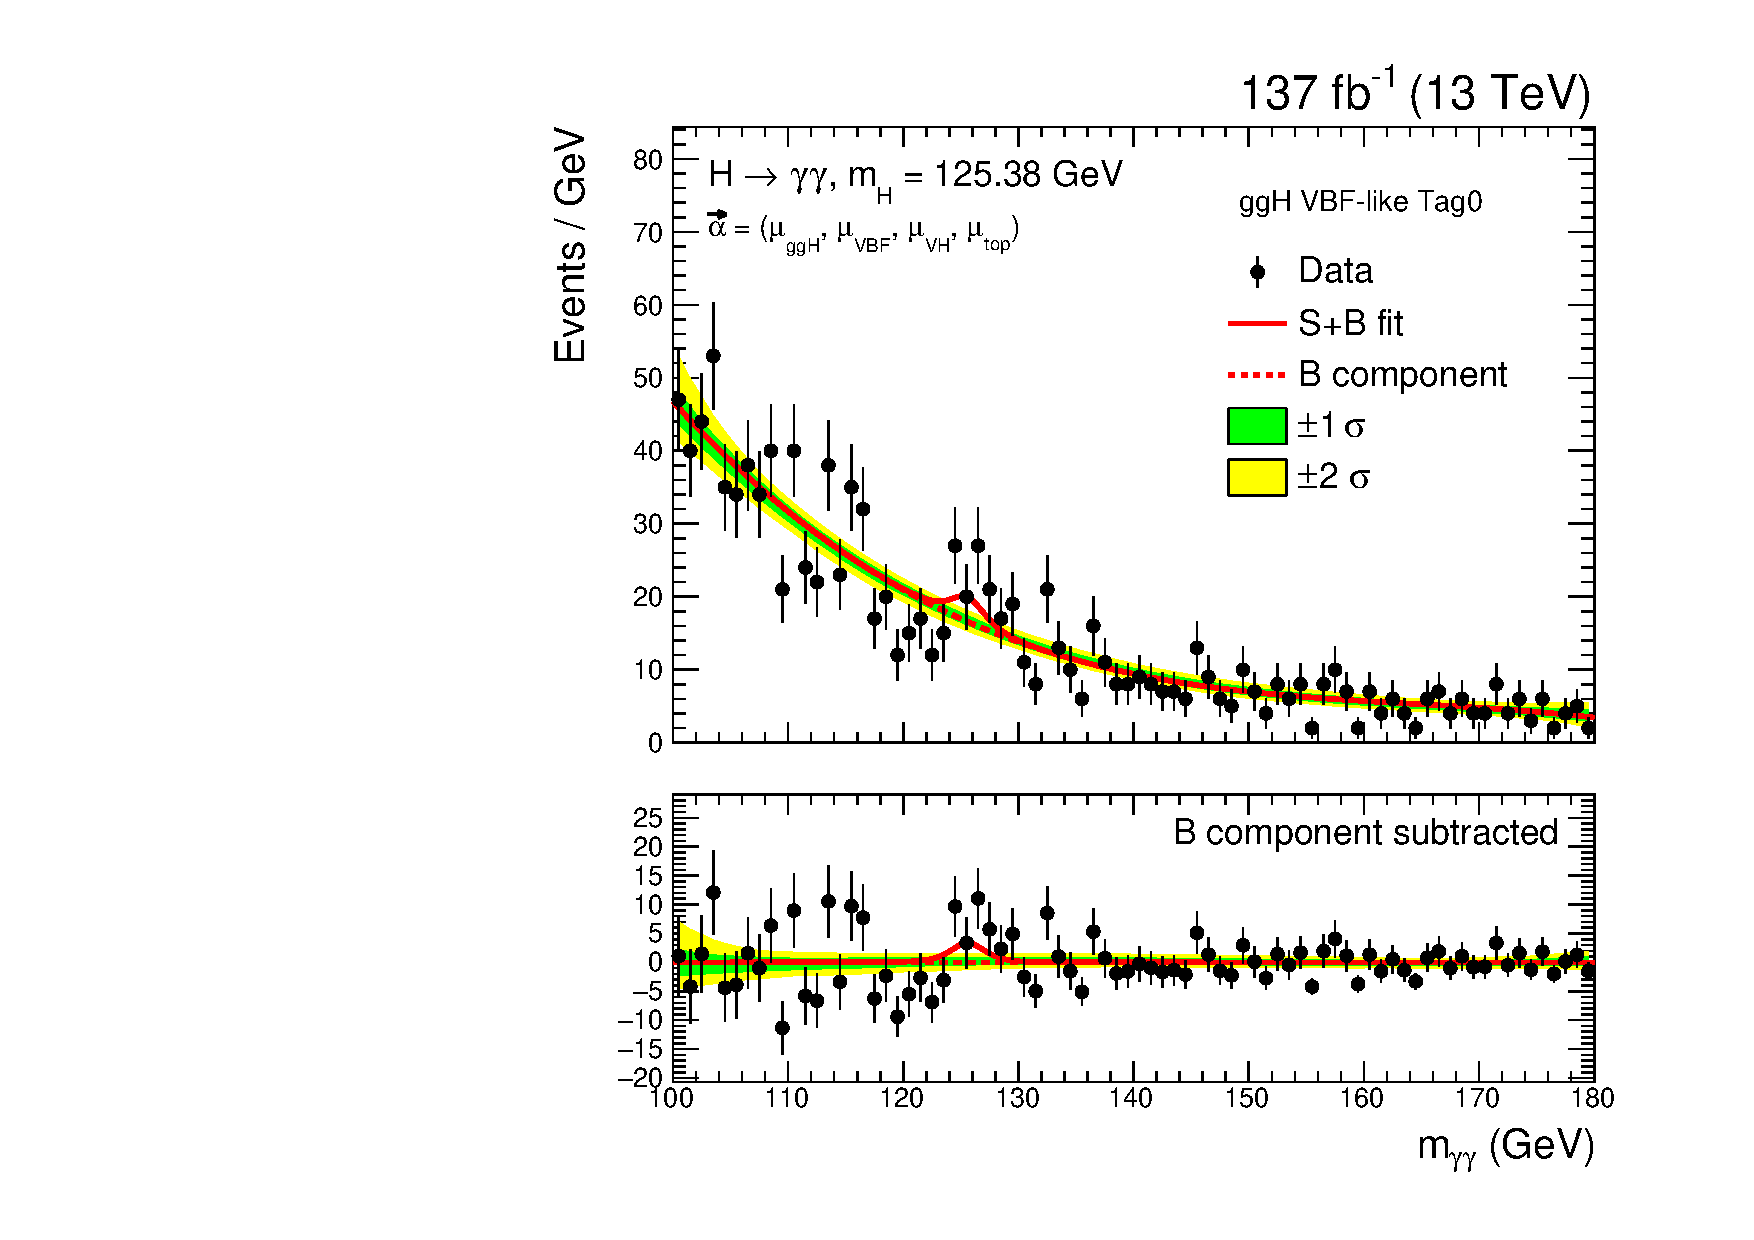
\includegraphics[width=.32\linewidth]{Figures/app_sb_models/RECO_VBFLIKEGGH_Tag0_CMS_hgg_mass.pdf}
  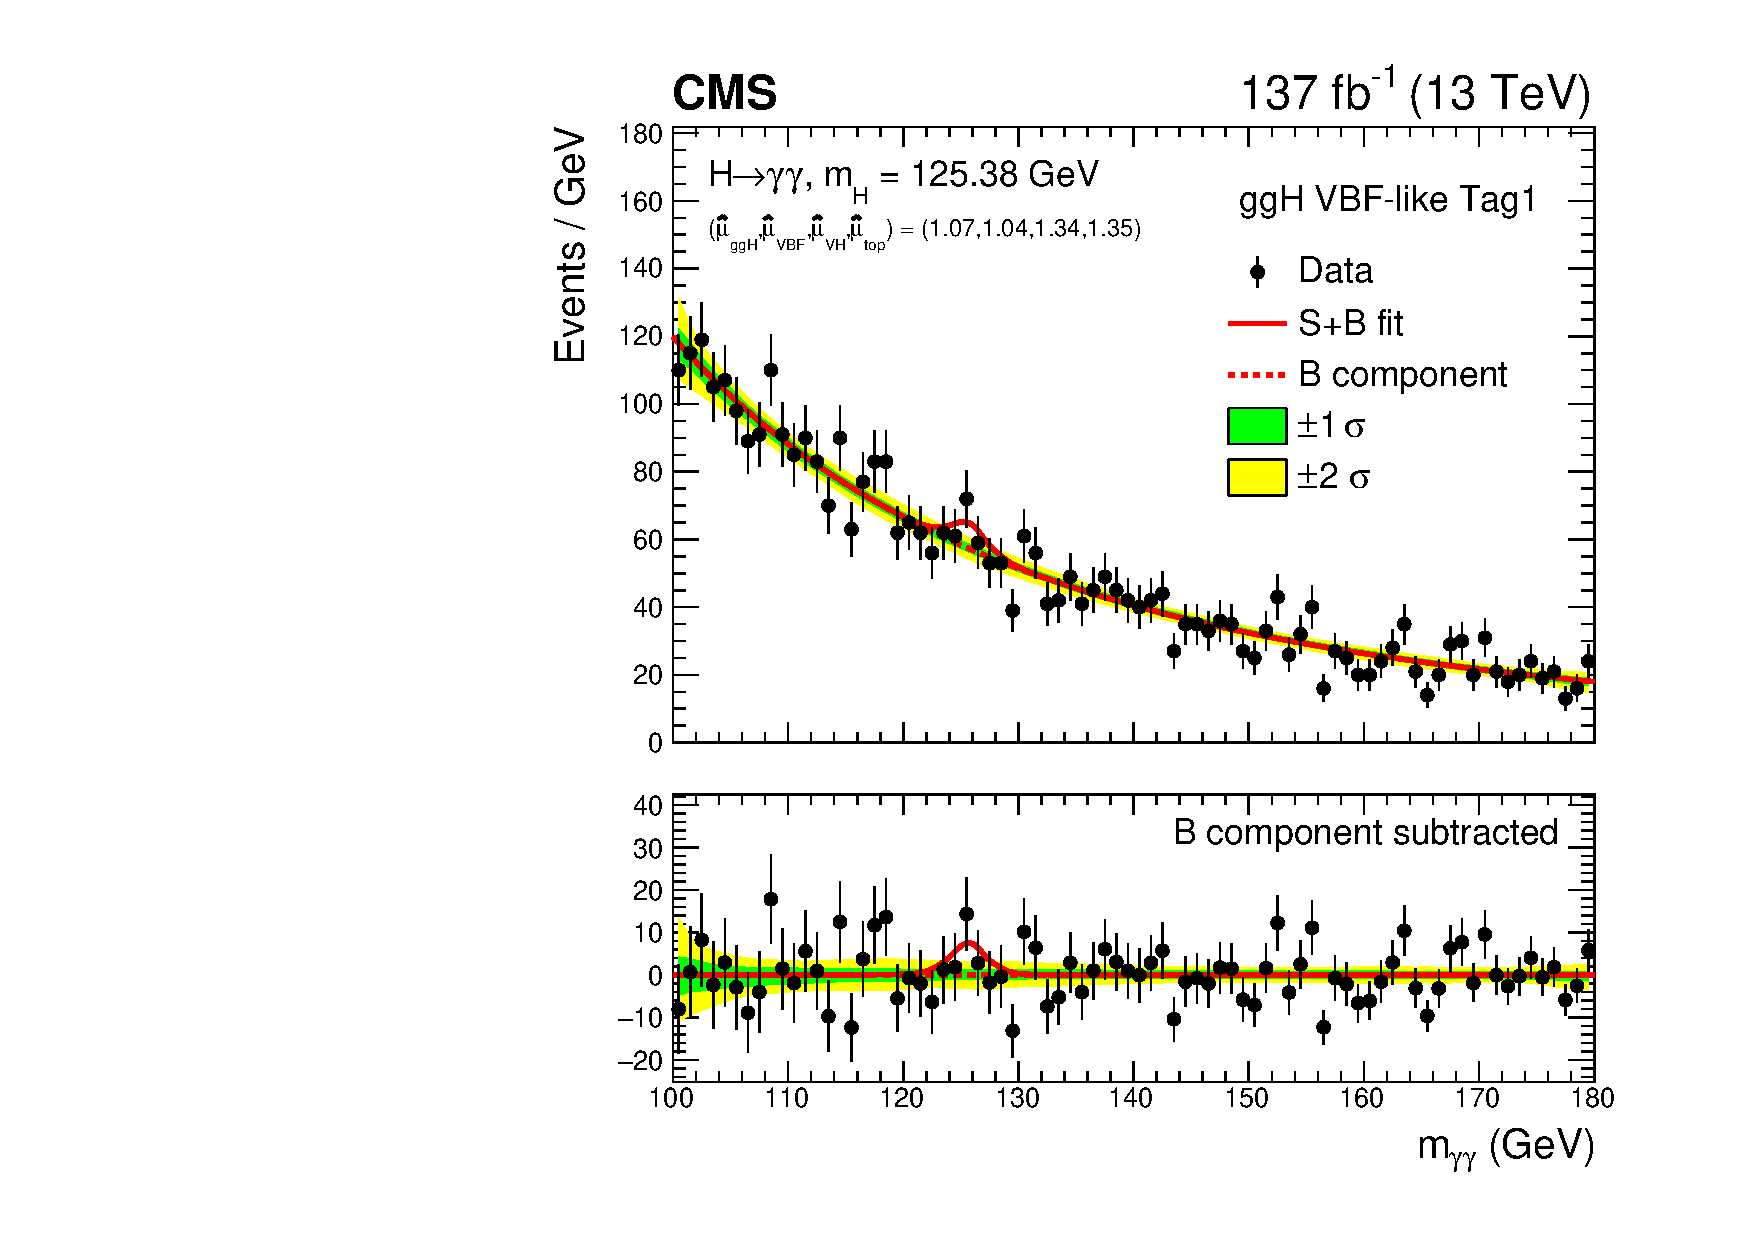
\includegraphics[width=.32\linewidth]{Figures/app_sb_models/RECO_VBFLIKEGGH_Tag1_CMS_hgg_mass.pdf}
  \caption[Observed diphoton mass distributions: ggH BSM and ggH VBF-like]
  {
    Data points (black) and the best-fit signal-plus-background model for the individual analysis categories targeting the ggH BSM and ggH VBF-like STXS regions. The best-fit model corresponds to the per-production mode signal strength fit. The solid red line shows the best-fit signal-plus-background model, whereas the dashed line shows the background component only. The one standard deviation (green) and two standard deviation (yellow) bands show the uncertainties in the background component of the fit. The bottom panels in each plot show the residuals after subtraction of this background component.
  }
  \label{fig:diphoton_mass_2}
\end{figure}

\begin{figure}[htbp]
  \centering
  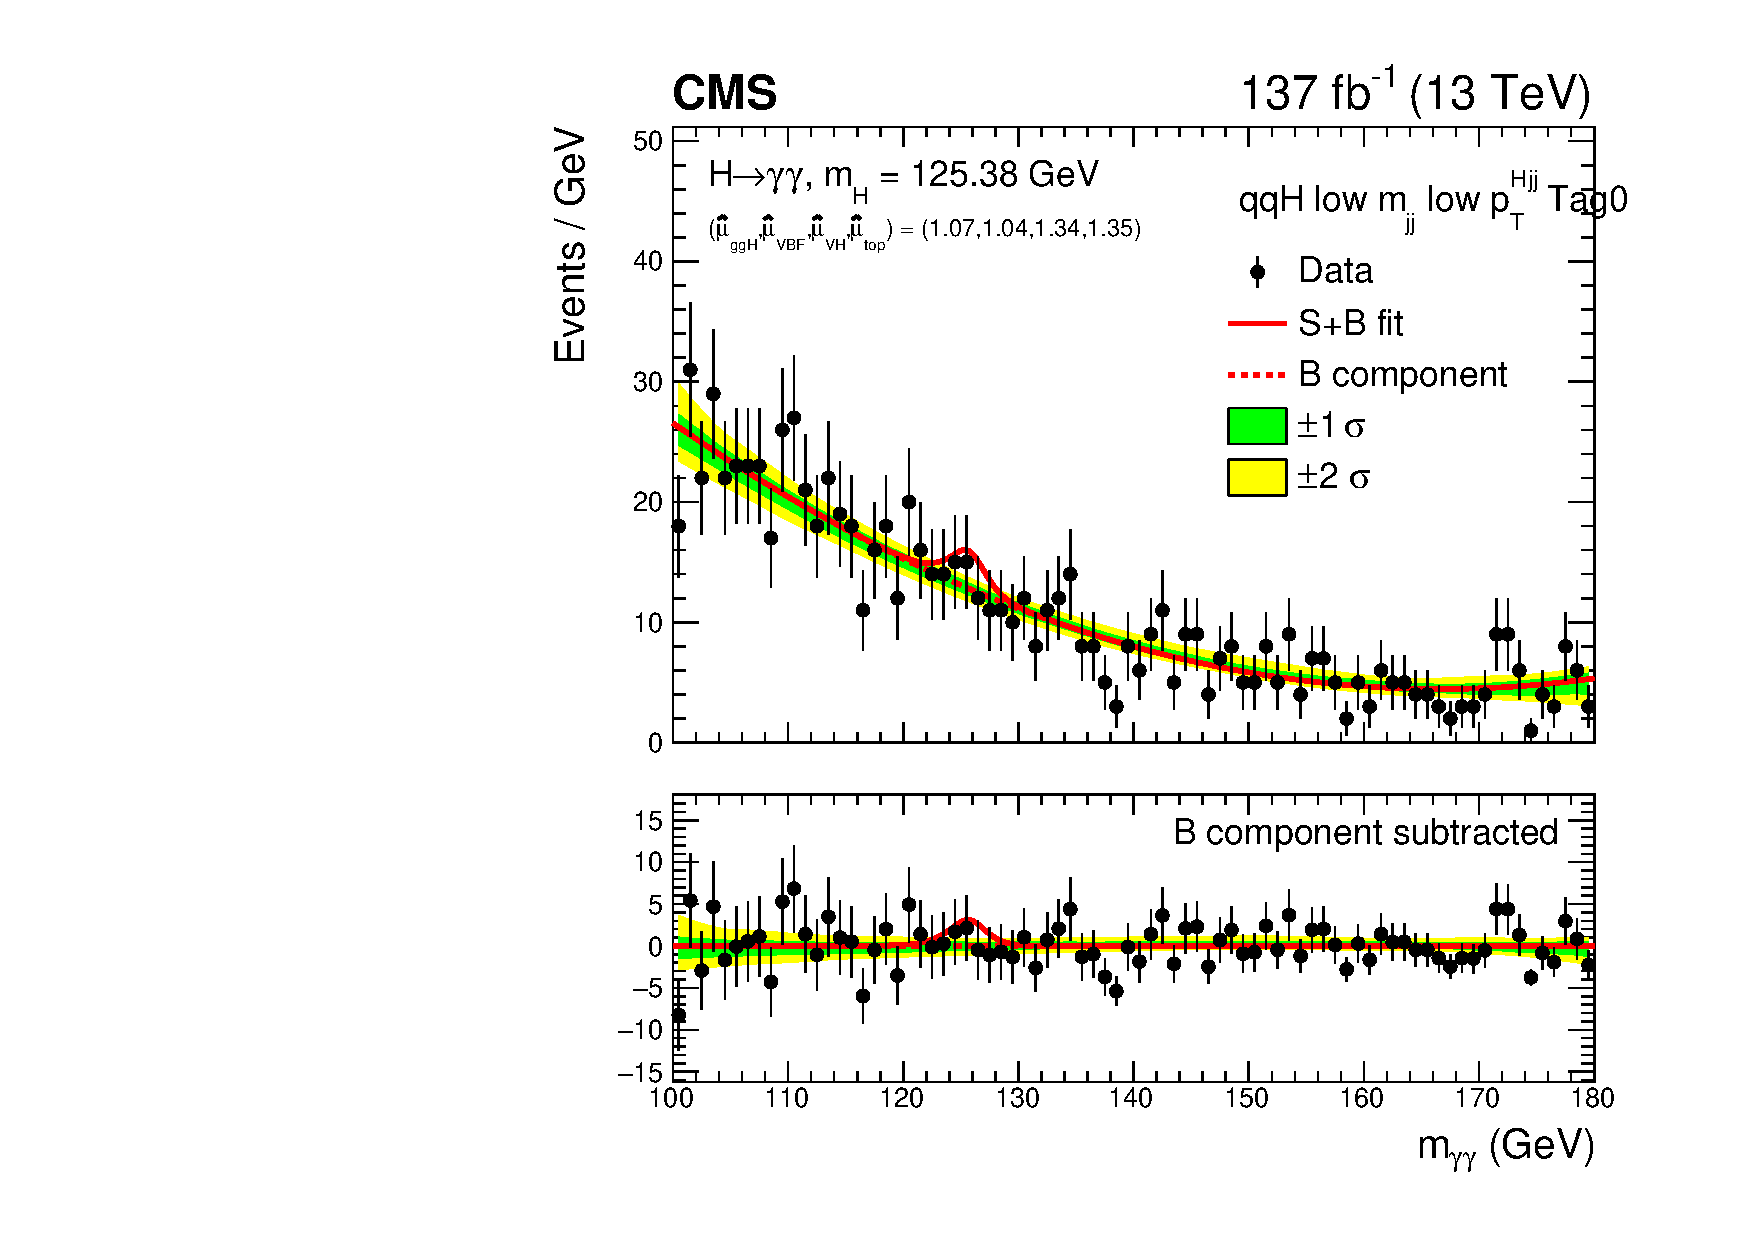
\includegraphics[width=.32\linewidth]{Figures/app_sb_models/RECO_VBFTOPO_JET3VETO_LOWMJJ_Tag0_CMS_hgg_mass.pdf}
  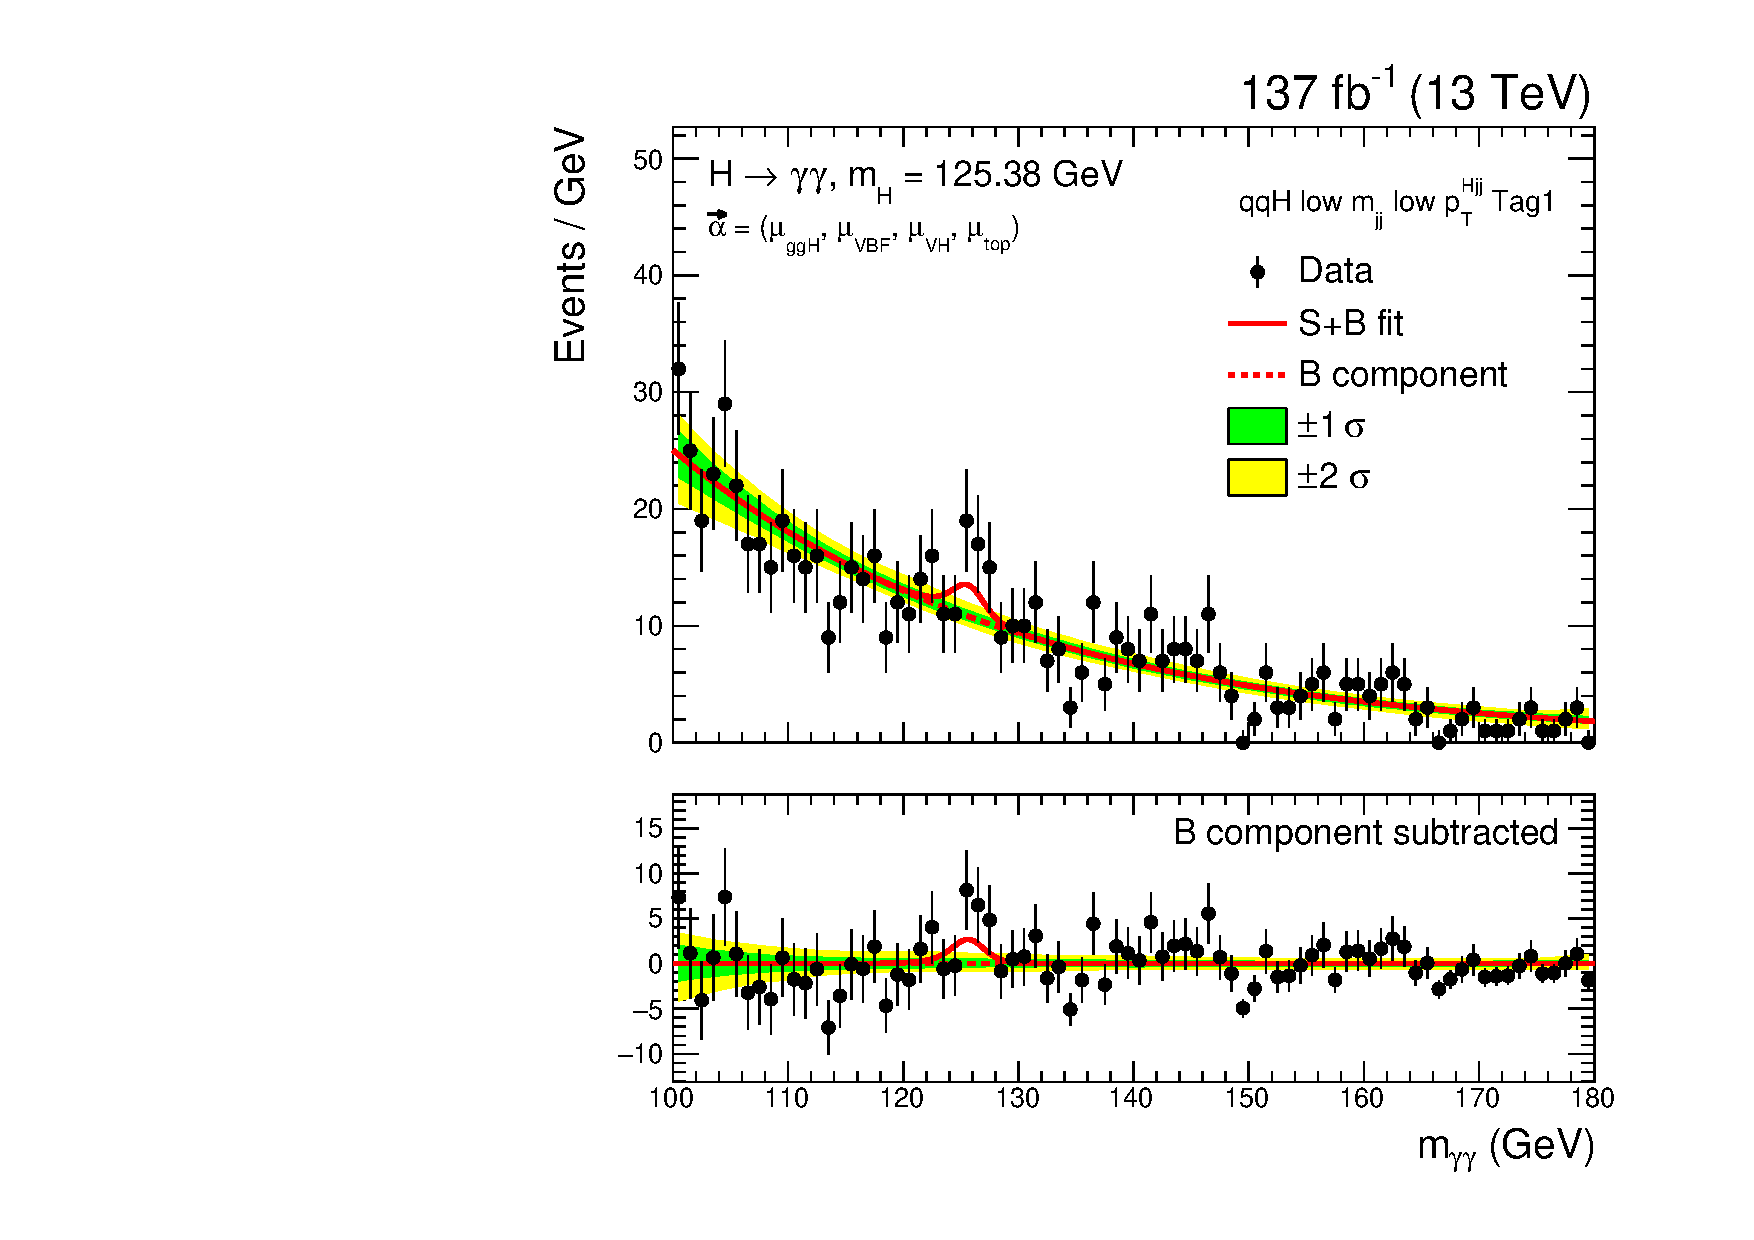
\includegraphics[width=.32\linewidth]{Figures/app_sb_models/RECO_VBFTOPO_JET3VETO_LOWMJJ_Tag1_CMS_hgg_mass.pdf}
  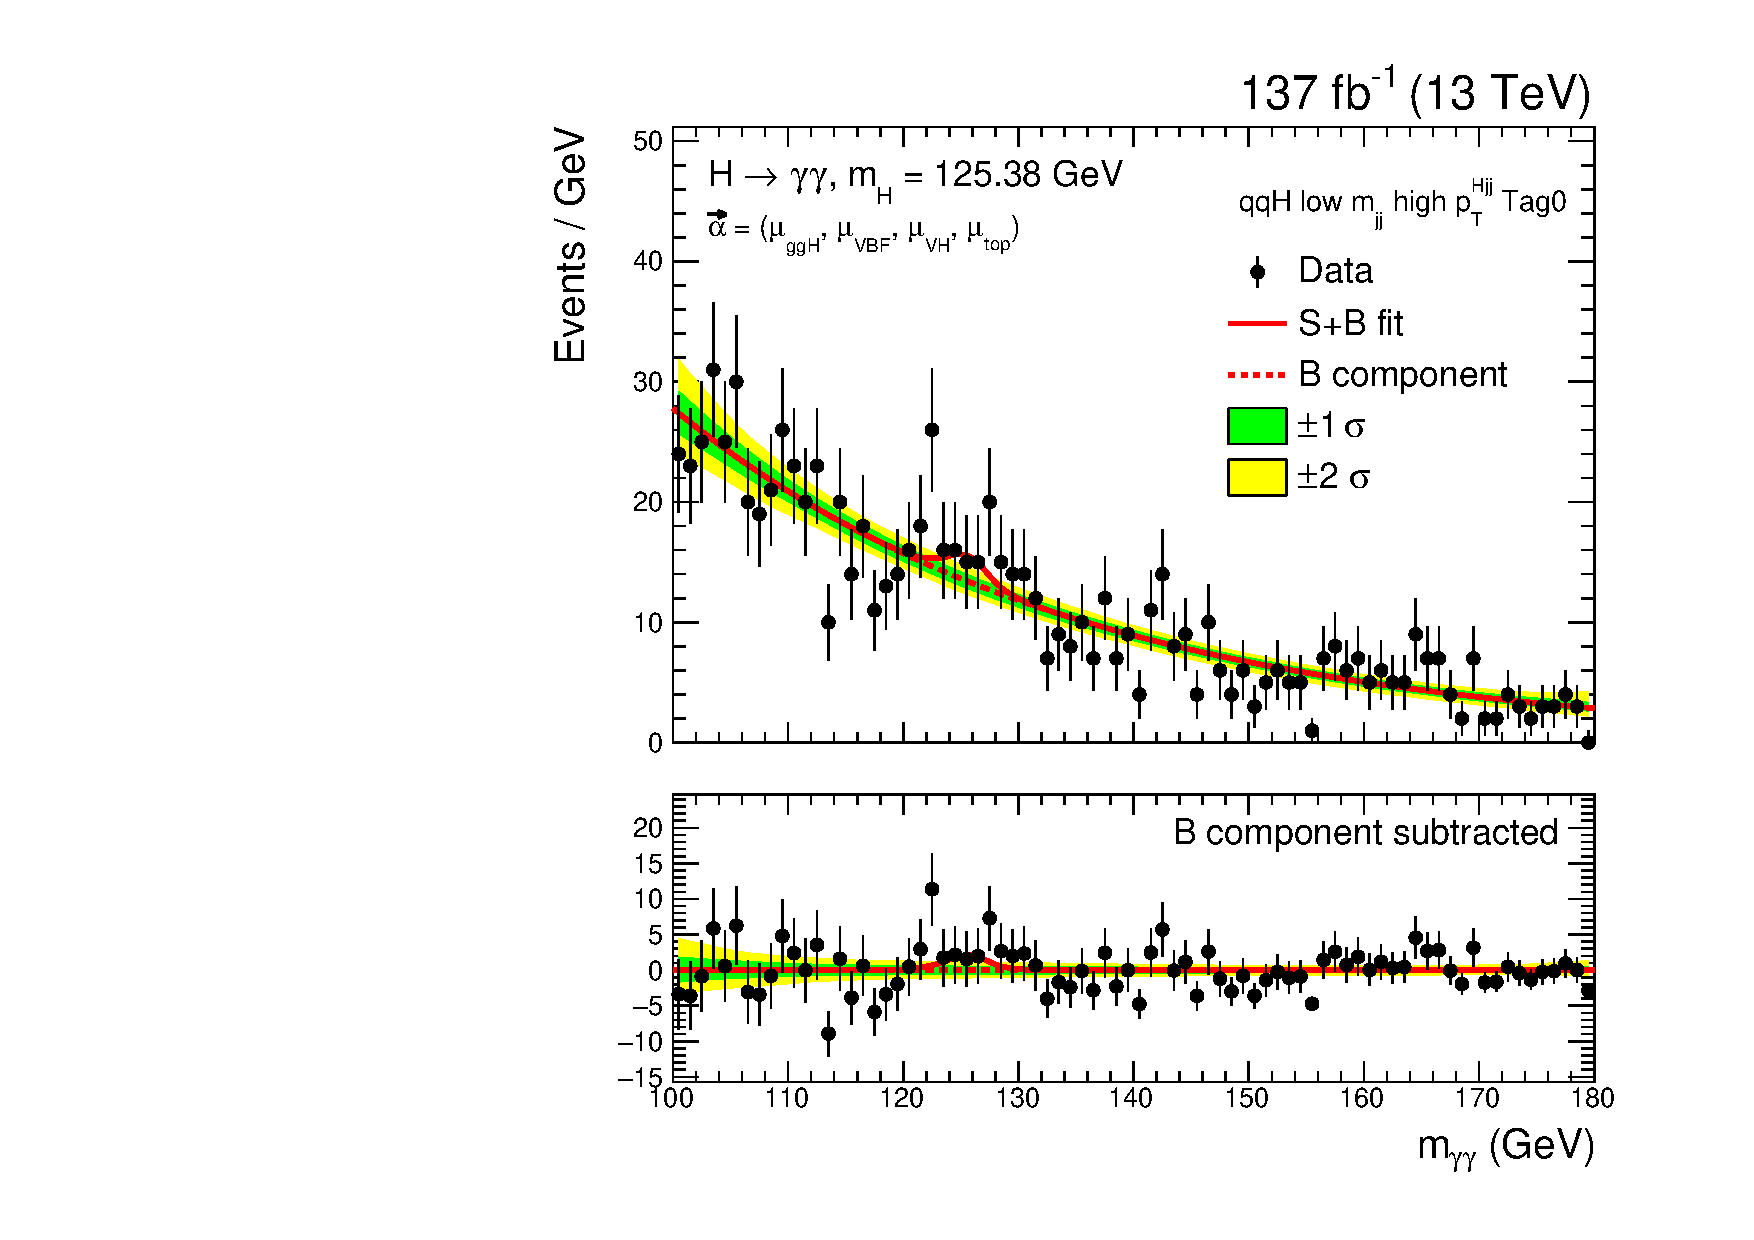
\includegraphics[width=.32\linewidth]{Figures/app_sb_models/RECO_VBFTOPO_JET3_LOWMJJ_Tag0_CMS_hgg_mass.pdf}
  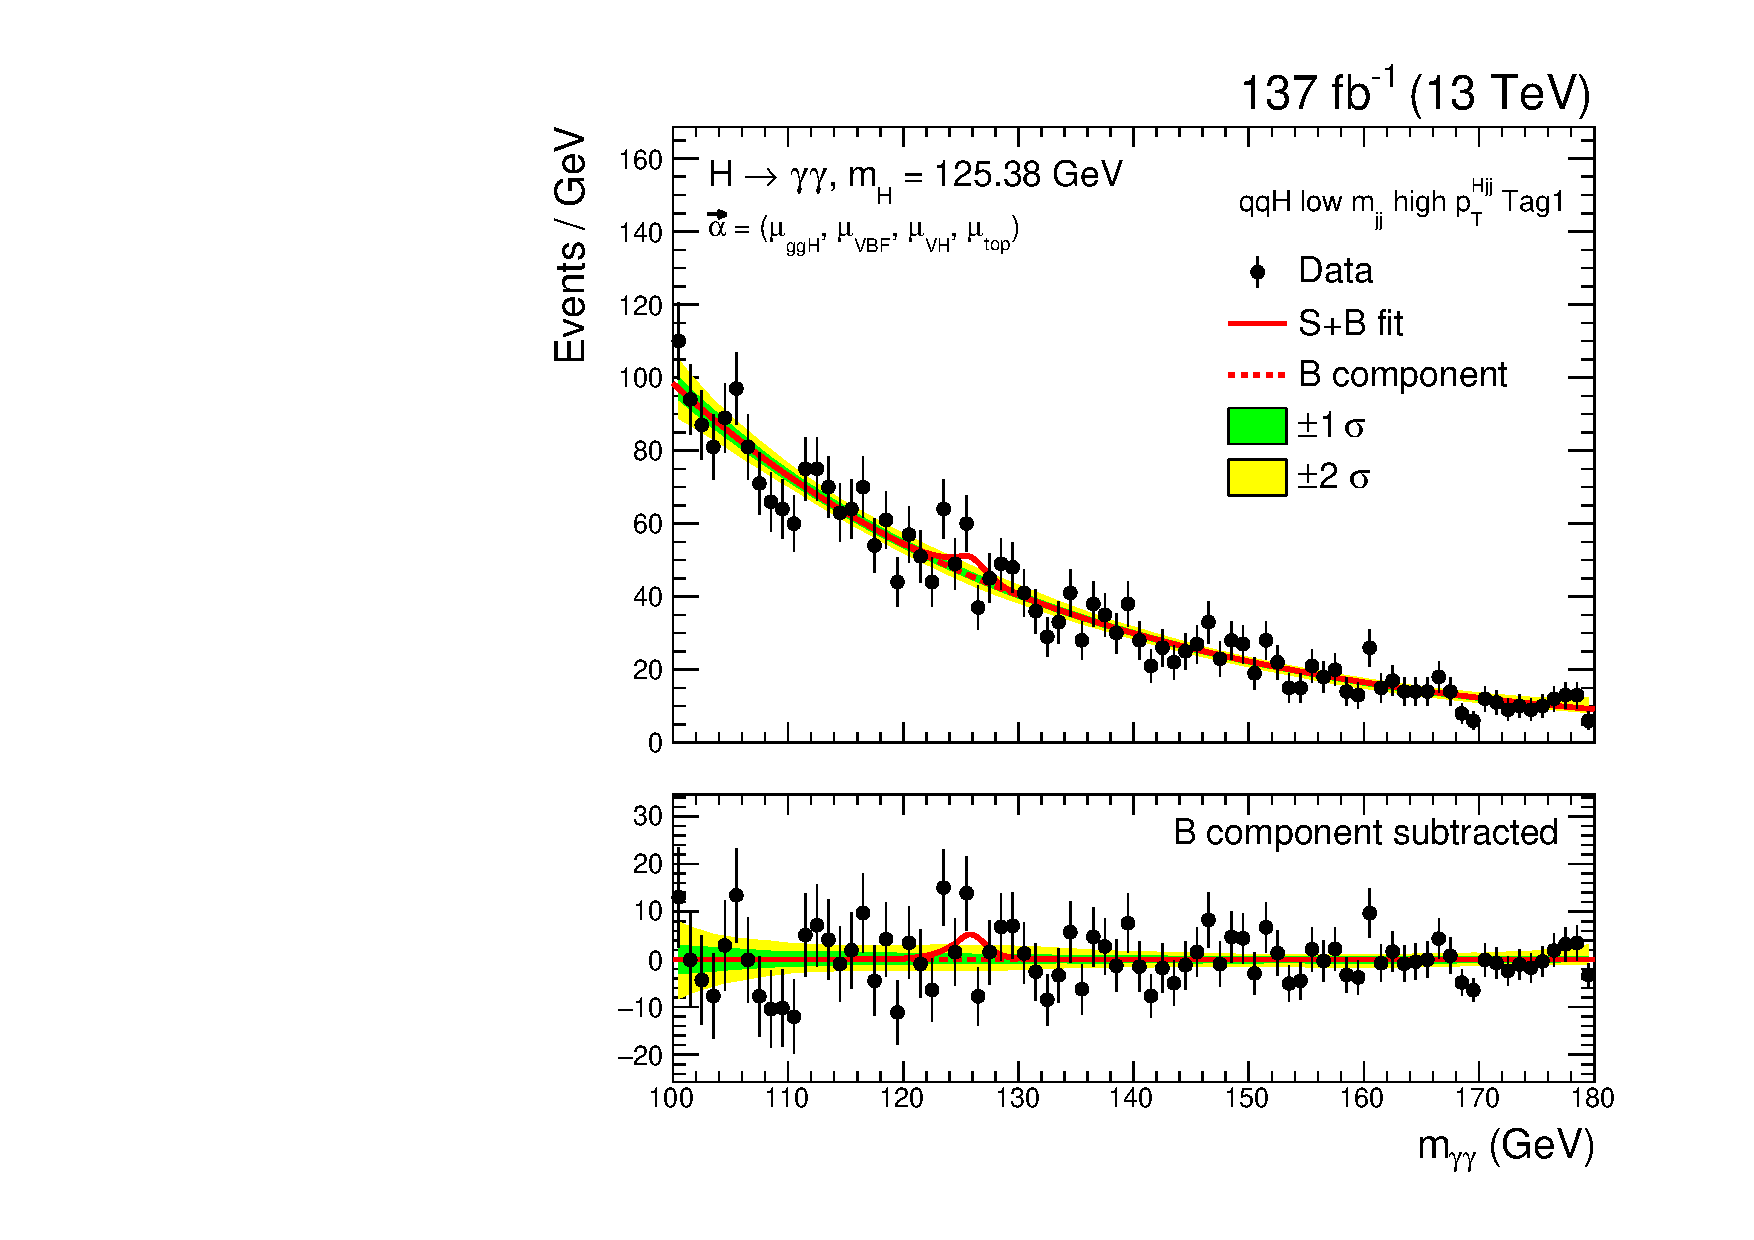
\includegraphics[width=.32\linewidth]{Figures/app_sb_models/RECO_VBFTOPO_JET3_LOWMJJ_Tag1_CMS_hgg_mass.pdf}
  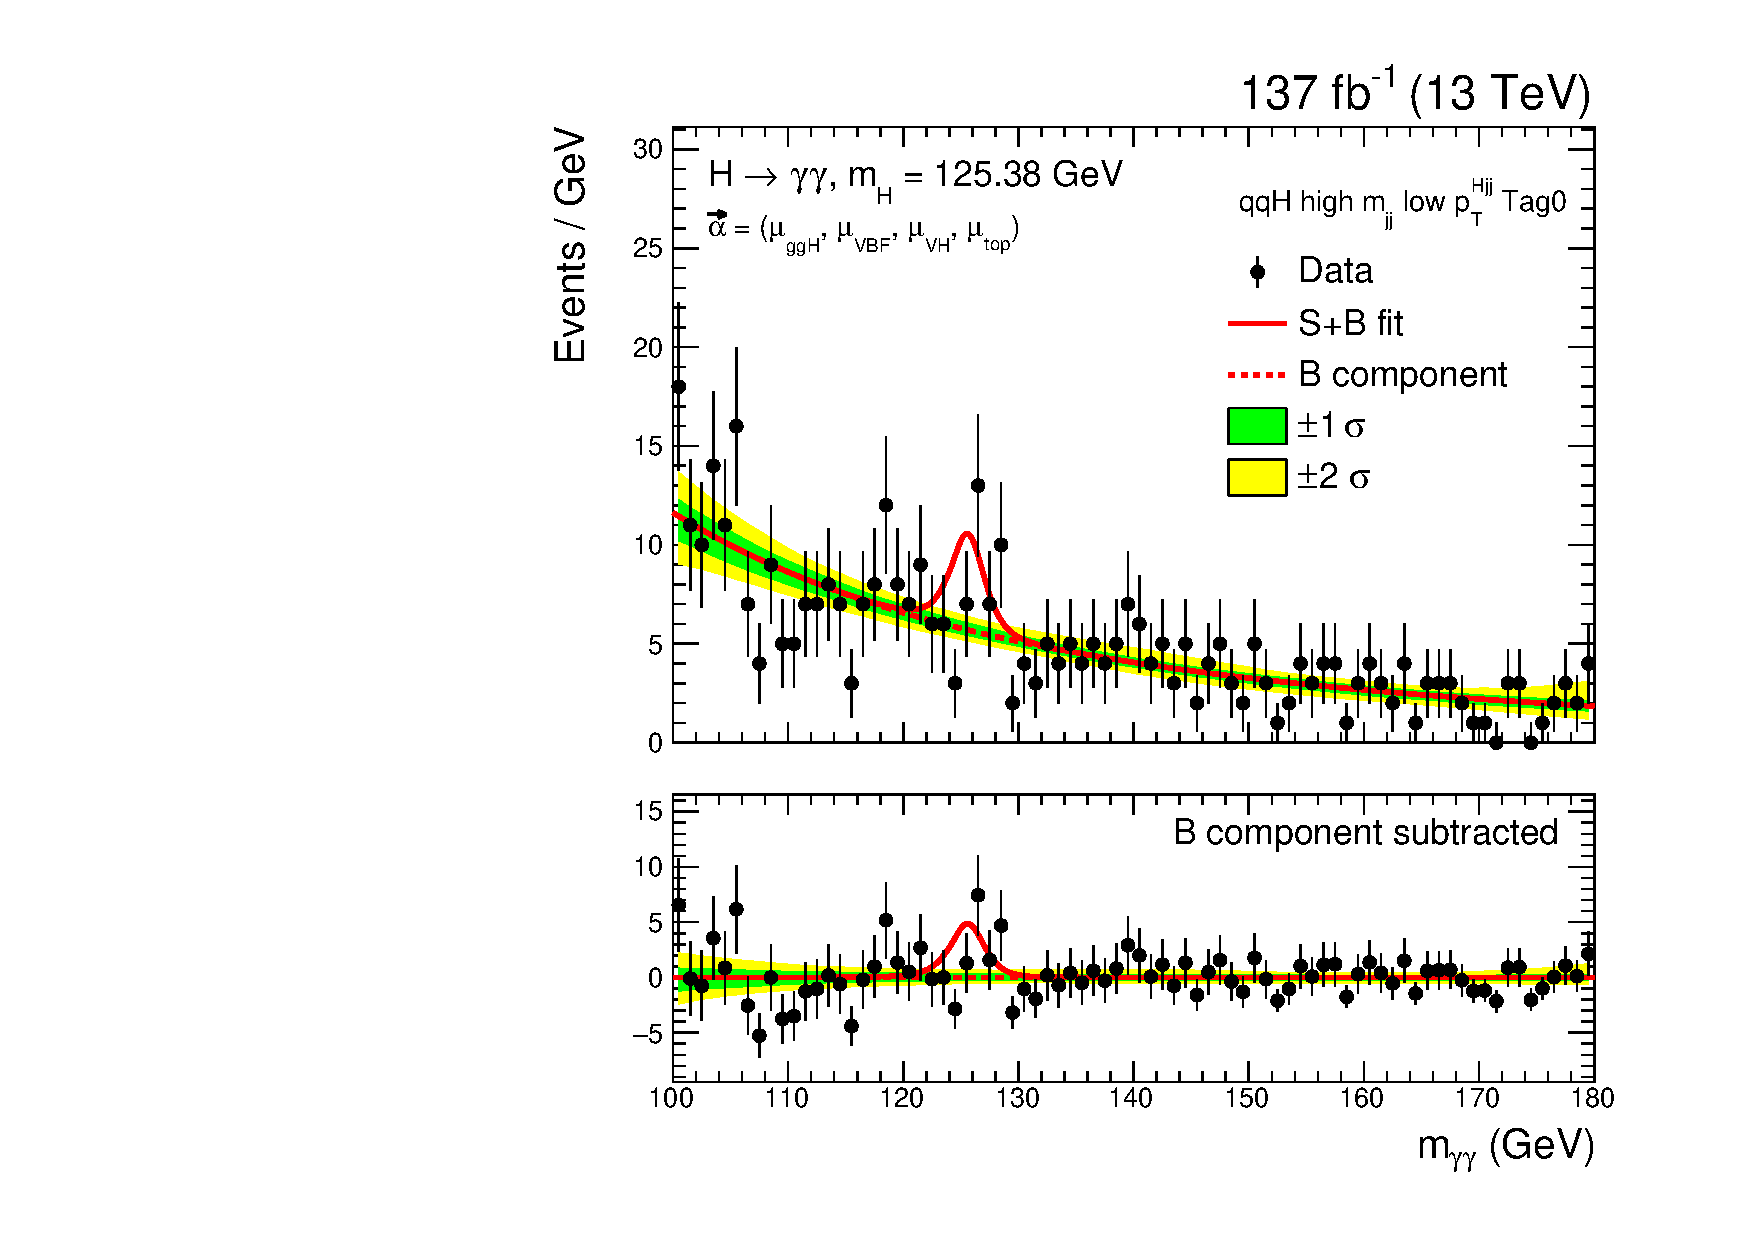
\includegraphics[width=.32\linewidth]{Figures/app_sb_models/RECO_VBFTOPO_JET3VETO_HIGHMJJ_Tag0_CMS_hgg_mass.pdf}
  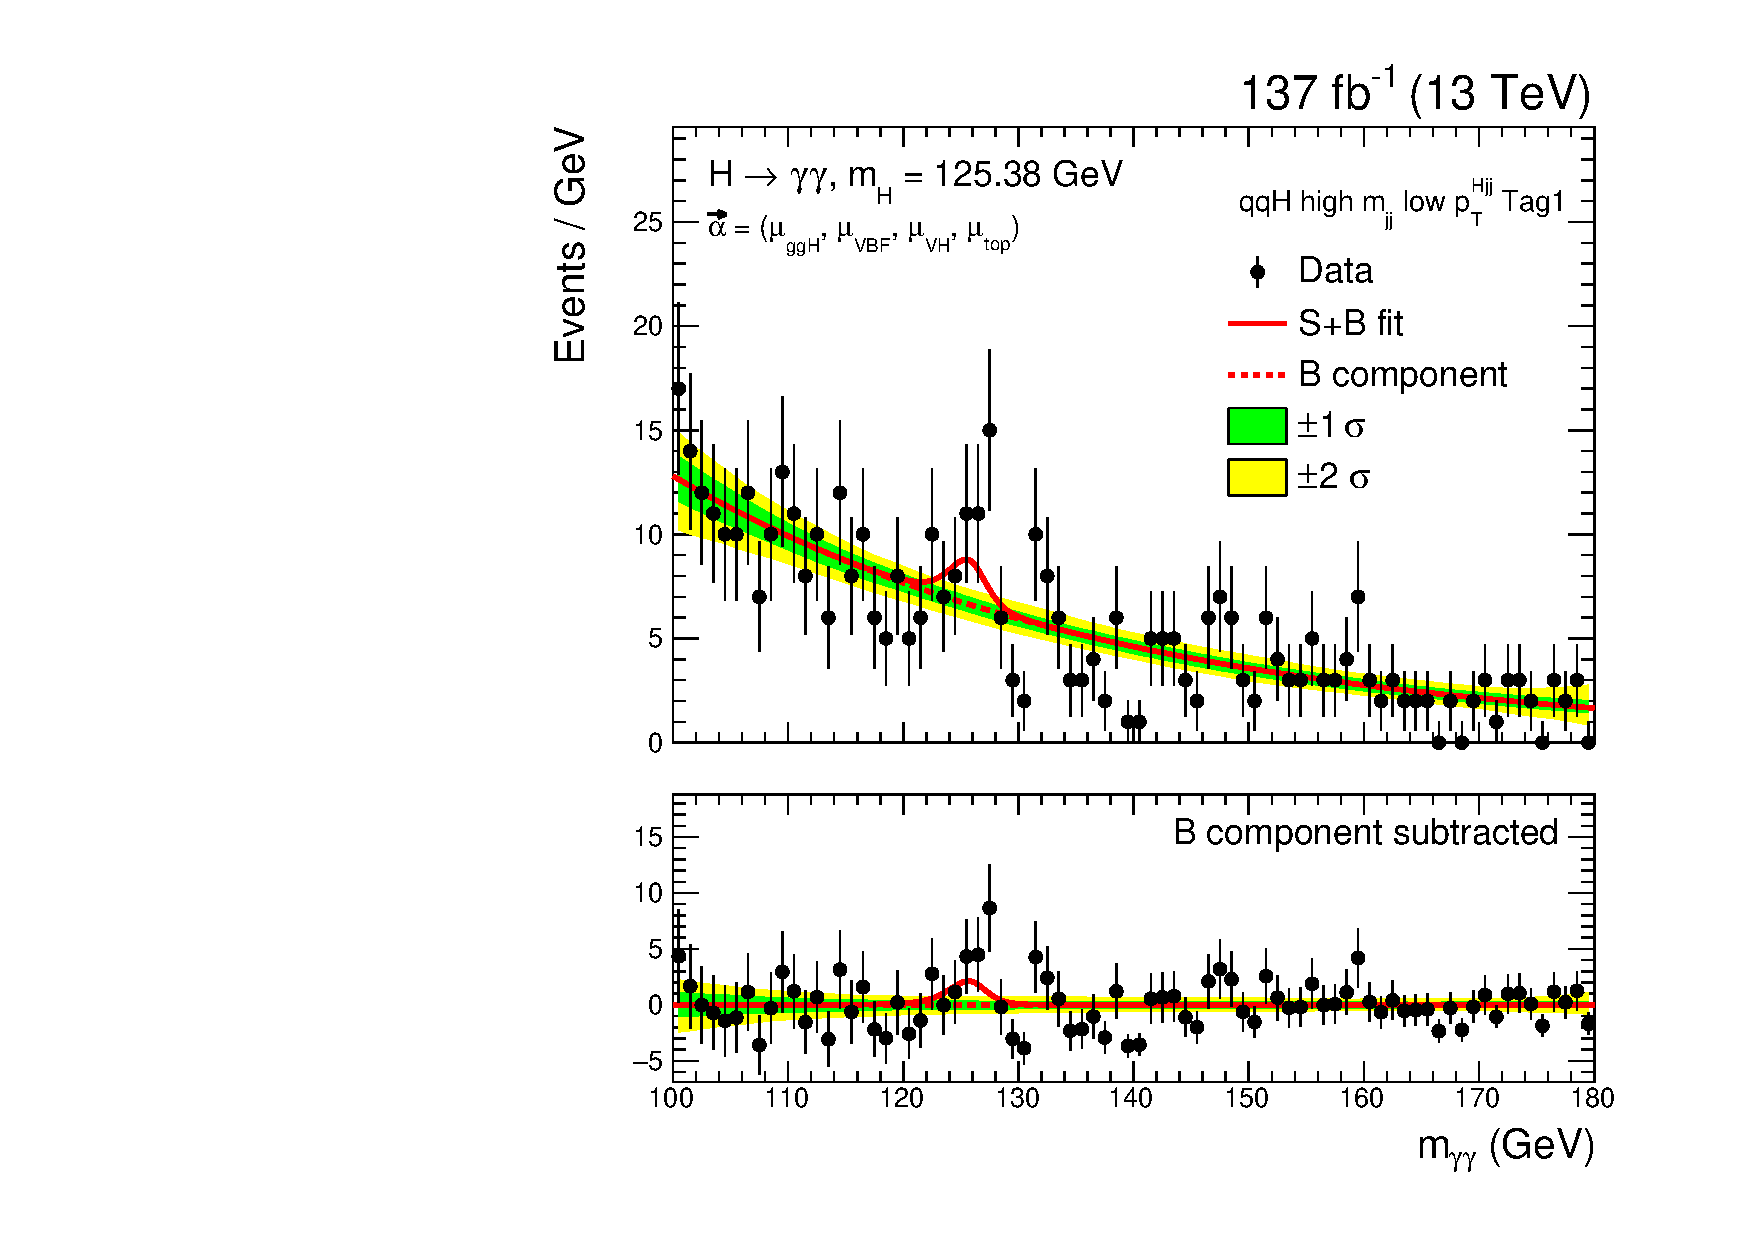
\includegraphics[width=.32\linewidth]{Figures/app_sb_models/RECO_VBFTOPO_JET3VETO_HIGHMJJ_Tag1_CMS_hgg_mass.pdf}
  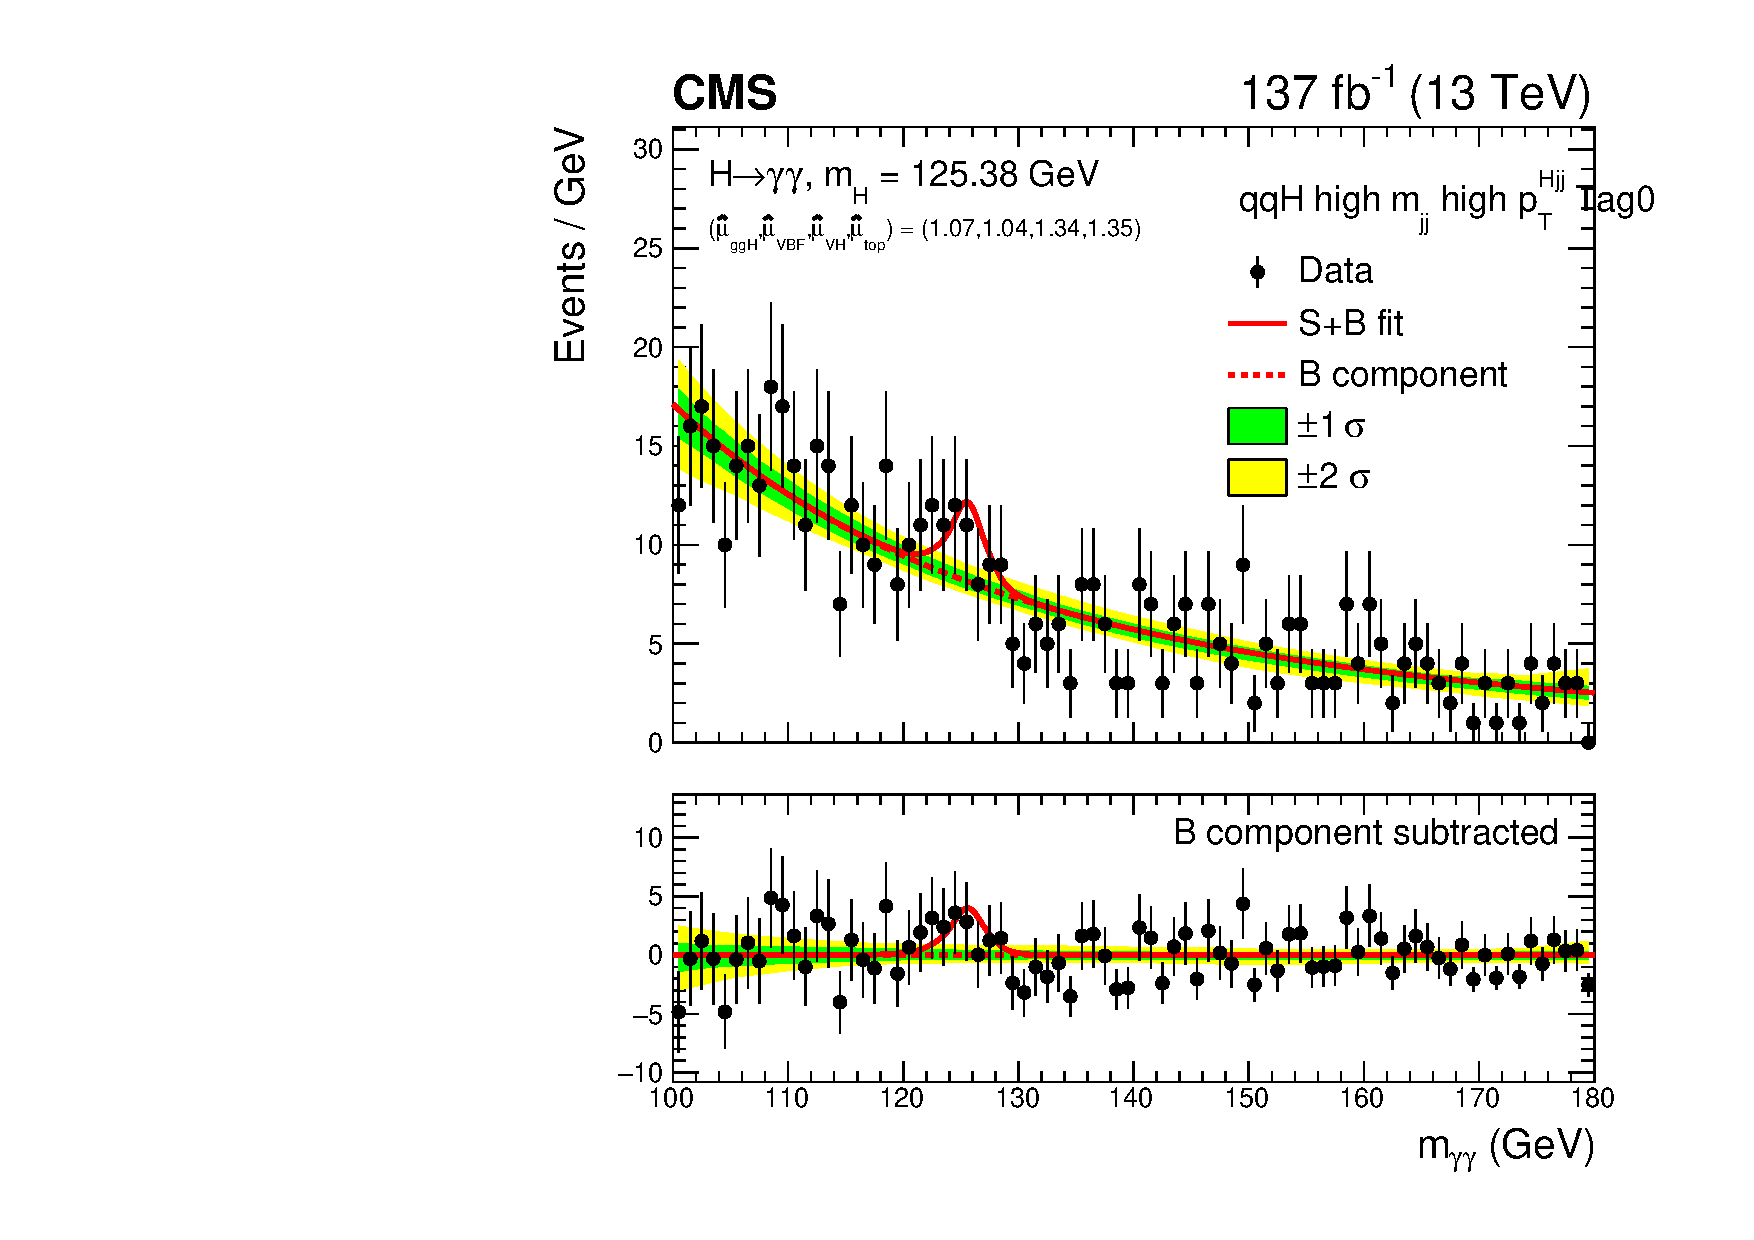
\includegraphics[width=.32\linewidth]{Figures/app_sb_models/RECO_VBFTOPO_JET3_HIGHMJJ_Tag0_CMS_hgg_mass.pdf}
  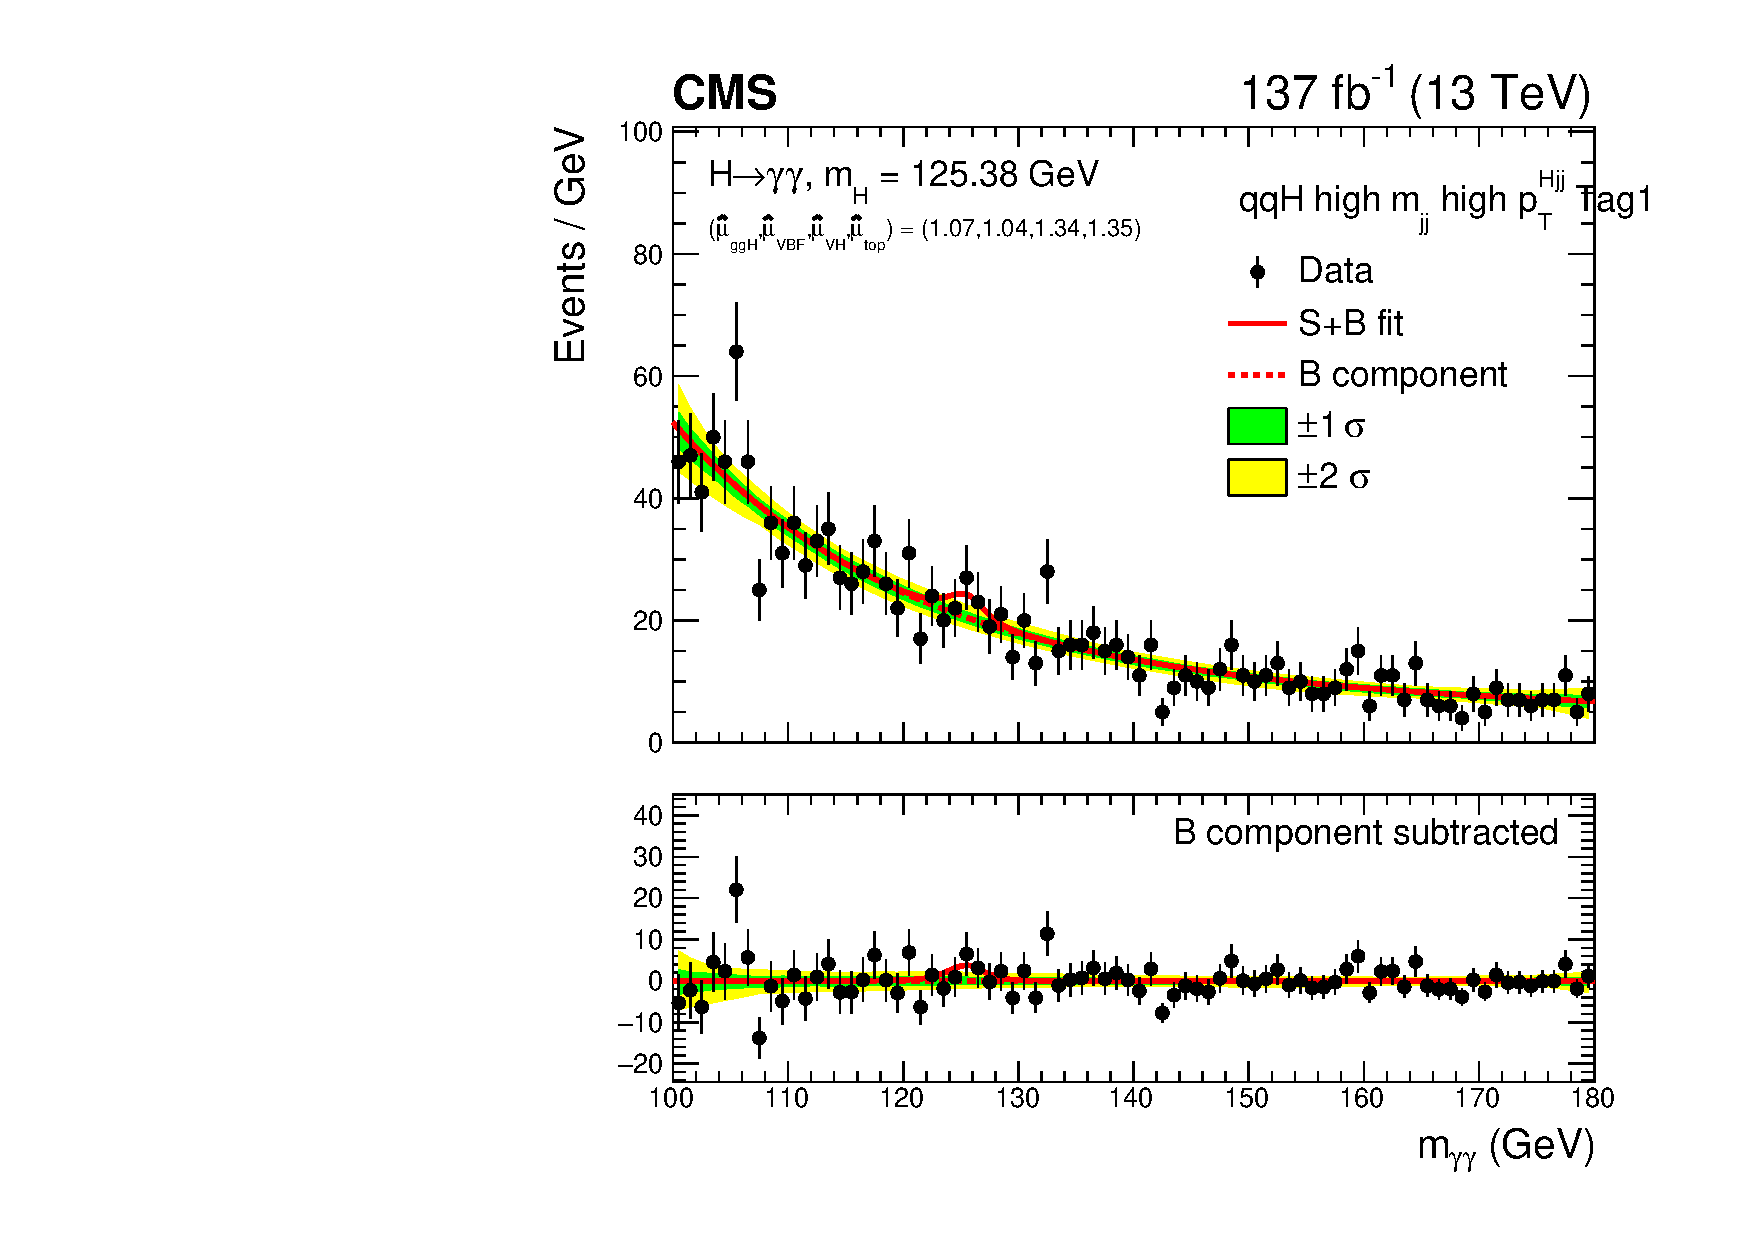
\includegraphics[width=.32\linewidth]{Figures/app_sb_models/RECO_VBFTOPO_JET3_HIGHMJJ_Tag1_CMS_hgg_mass.pdf}
  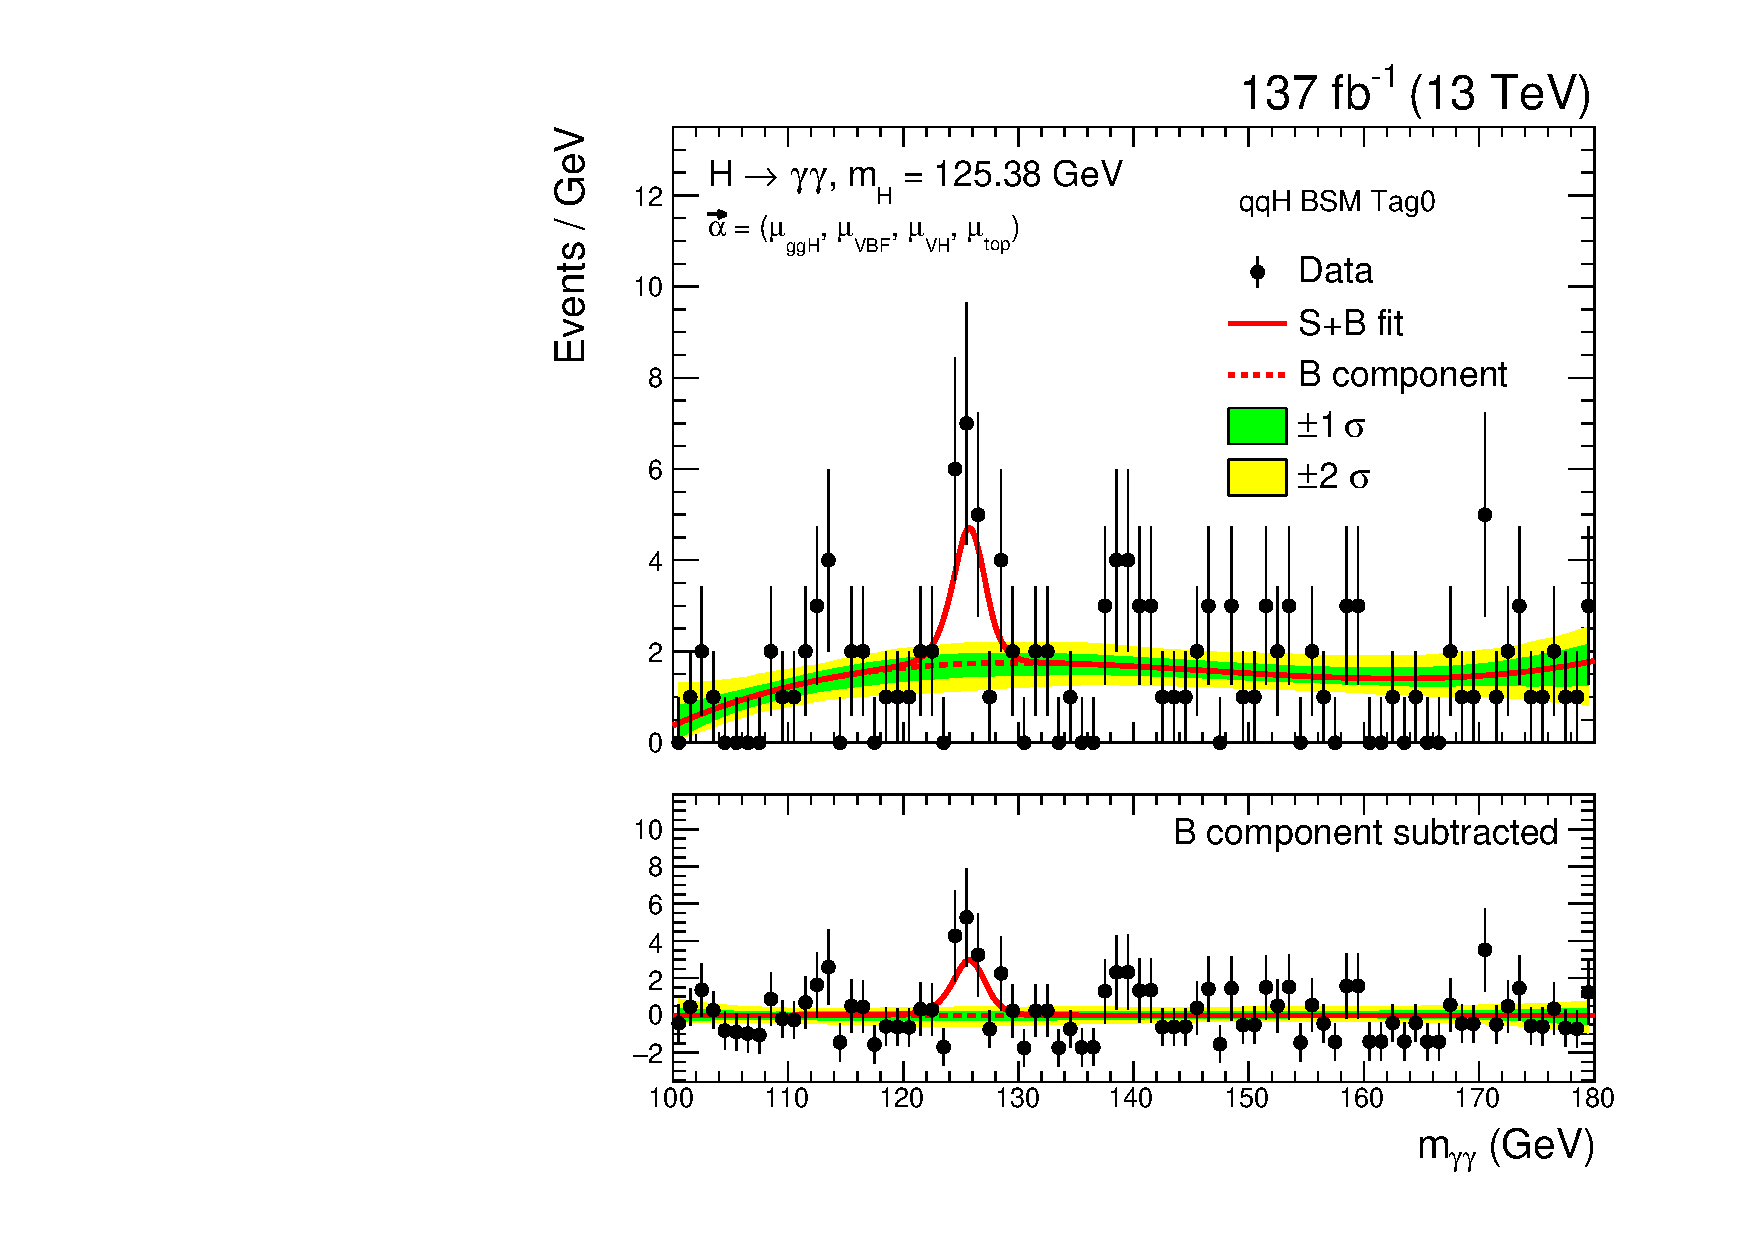
\includegraphics[width=.32\linewidth]{Figures/app_sb_models/RECO_VBFTOPO_BSM_Tag0_CMS_hgg_mass.pdf}
  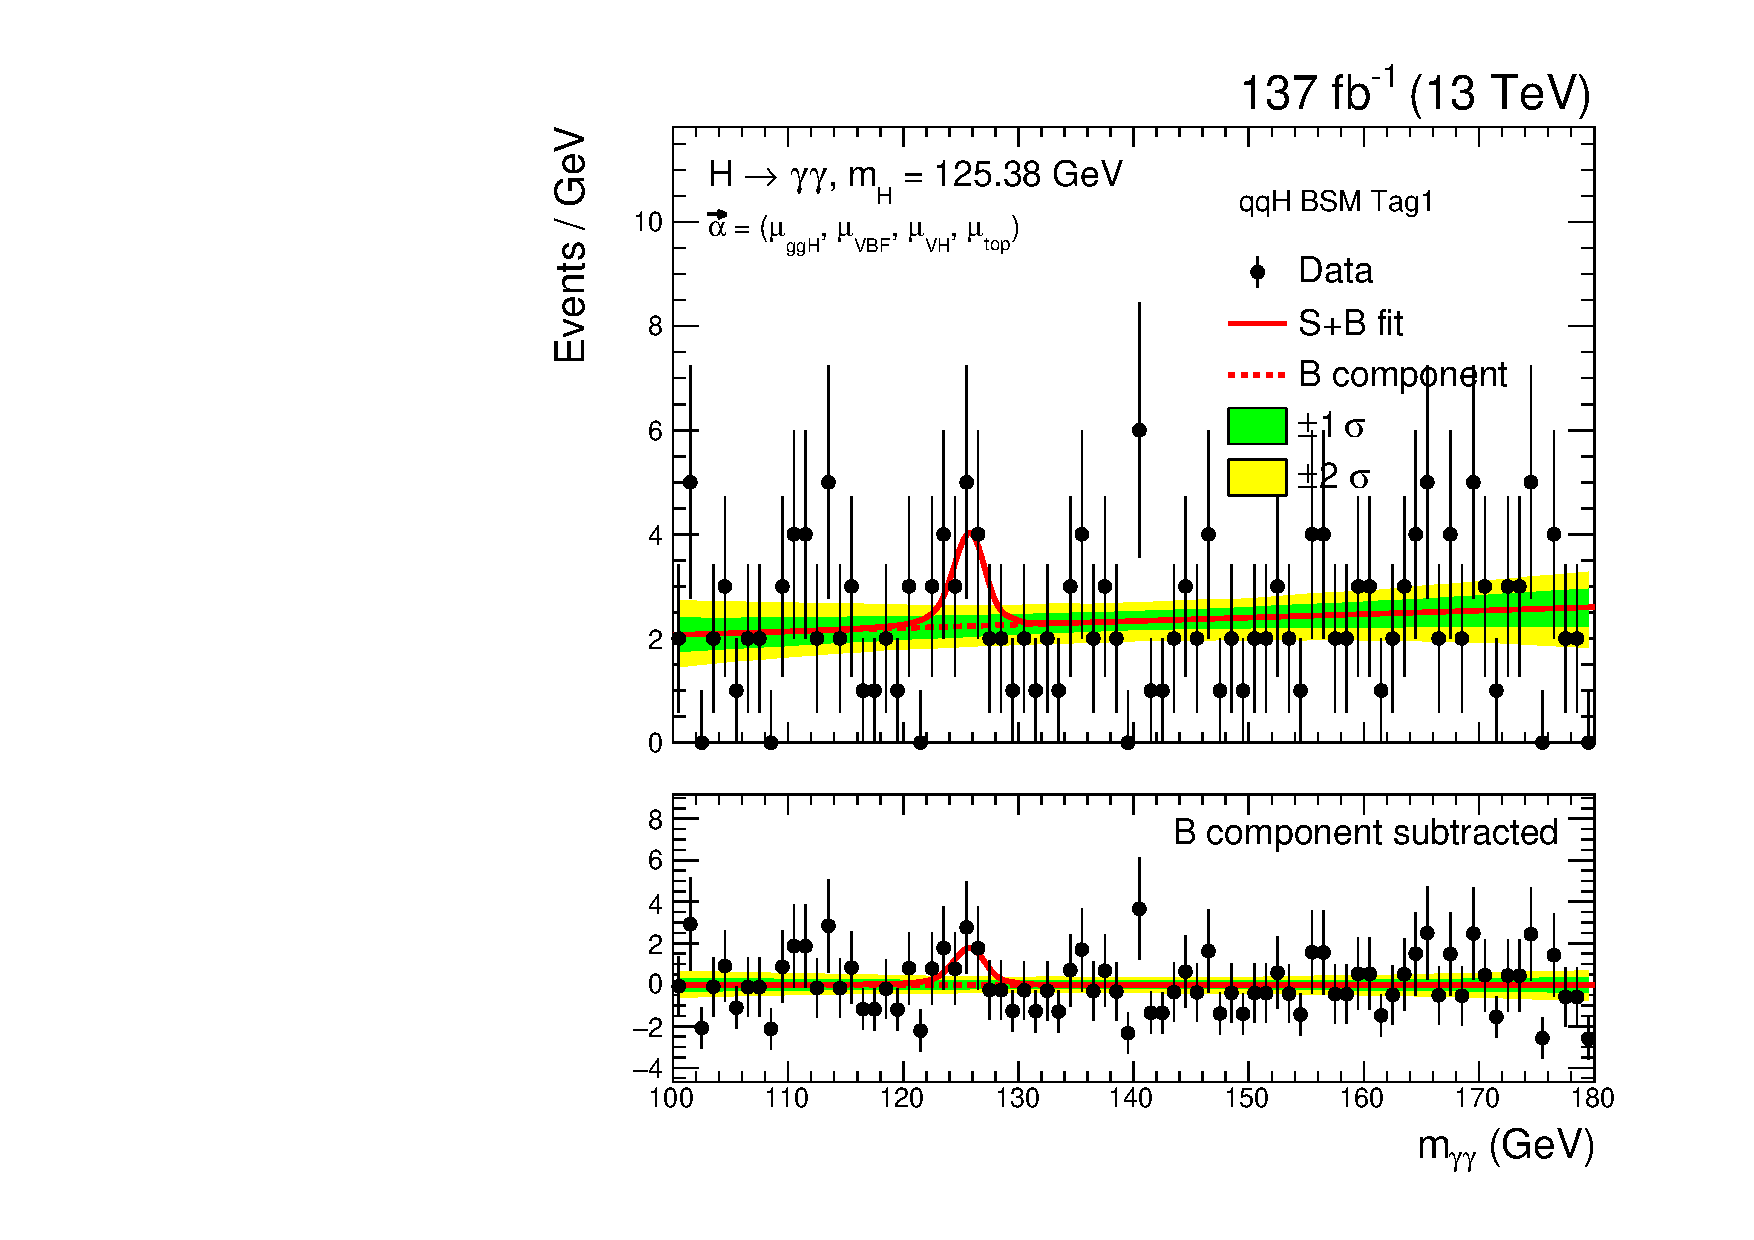
\includegraphics[width=.32\linewidth]{Figures/app_sb_models/RECO_VBFTOPO_BSM_Tag1_CMS_hgg_mass.pdf}
  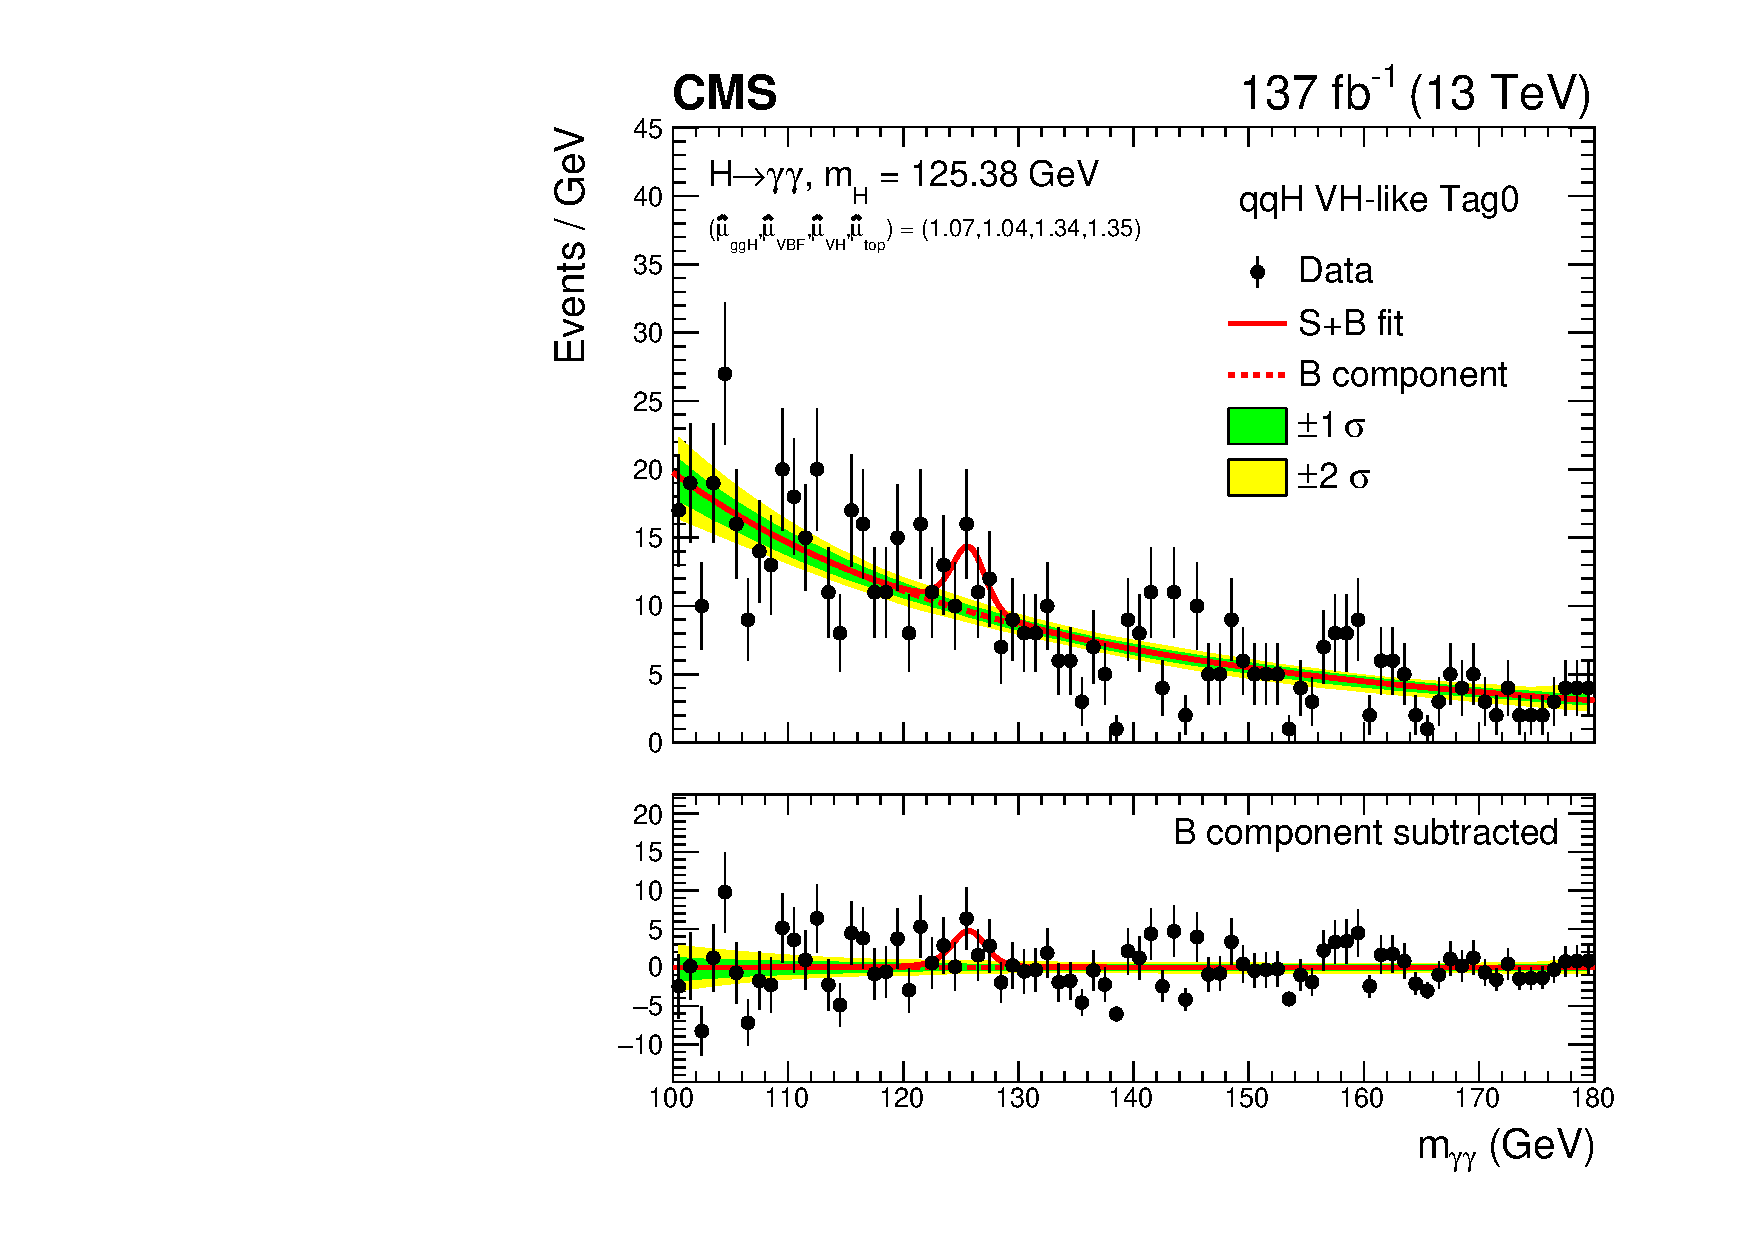
\includegraphics[width=.32\linewidth]{Figures/app_sb_models/RECO_VBFTOPO_VHHAD_Tag0_CMS_hgg_mass.pdf}
  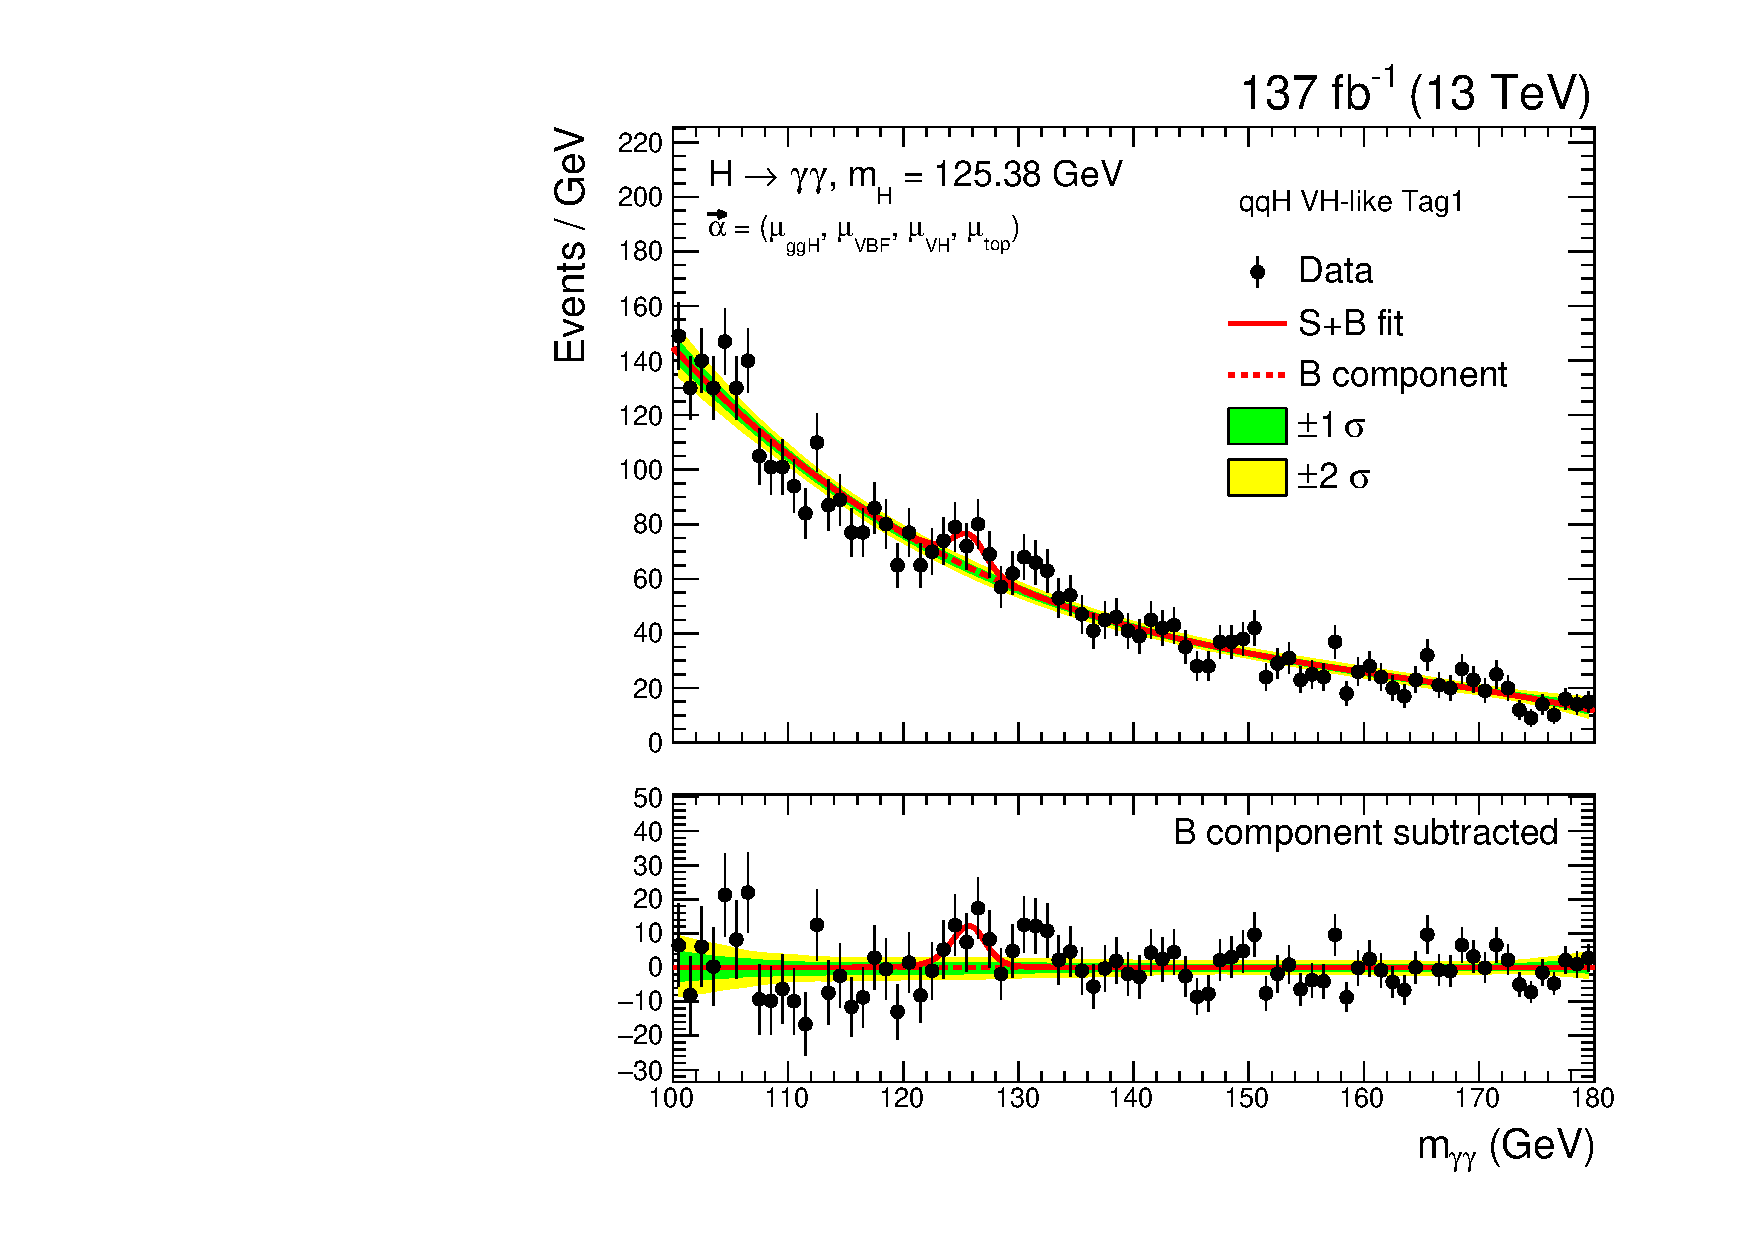
\includegraphics[width=.32\linewidth]{Figures/app_sb_models/RECO_VBFTOPO_VHHAD_Tag1_CMS_hgg_mass.pdf}
  \caption[Observed diphoton mass distributions: qqH]
  {
    Data points (black) and the best-fit signal-plus-background model for the individual analysis categories targeting the qqH STXS regions. The best-fit model corresponds to the per-production mode signal strength fit. The solid red line shows the best-fit signal-plus-background model, whereas the dashed line shows the background component only. The one standard deviation (green) and two standard deviation (yellow) bands show the uncertainties in the background component of the fit. The bottom panels in each plot show the residuals after subtraction of this background component.
  }
  \label{fig:diphoton_mass_3}
\end{figure}

\begin{figure}[htbp]
  \centering
  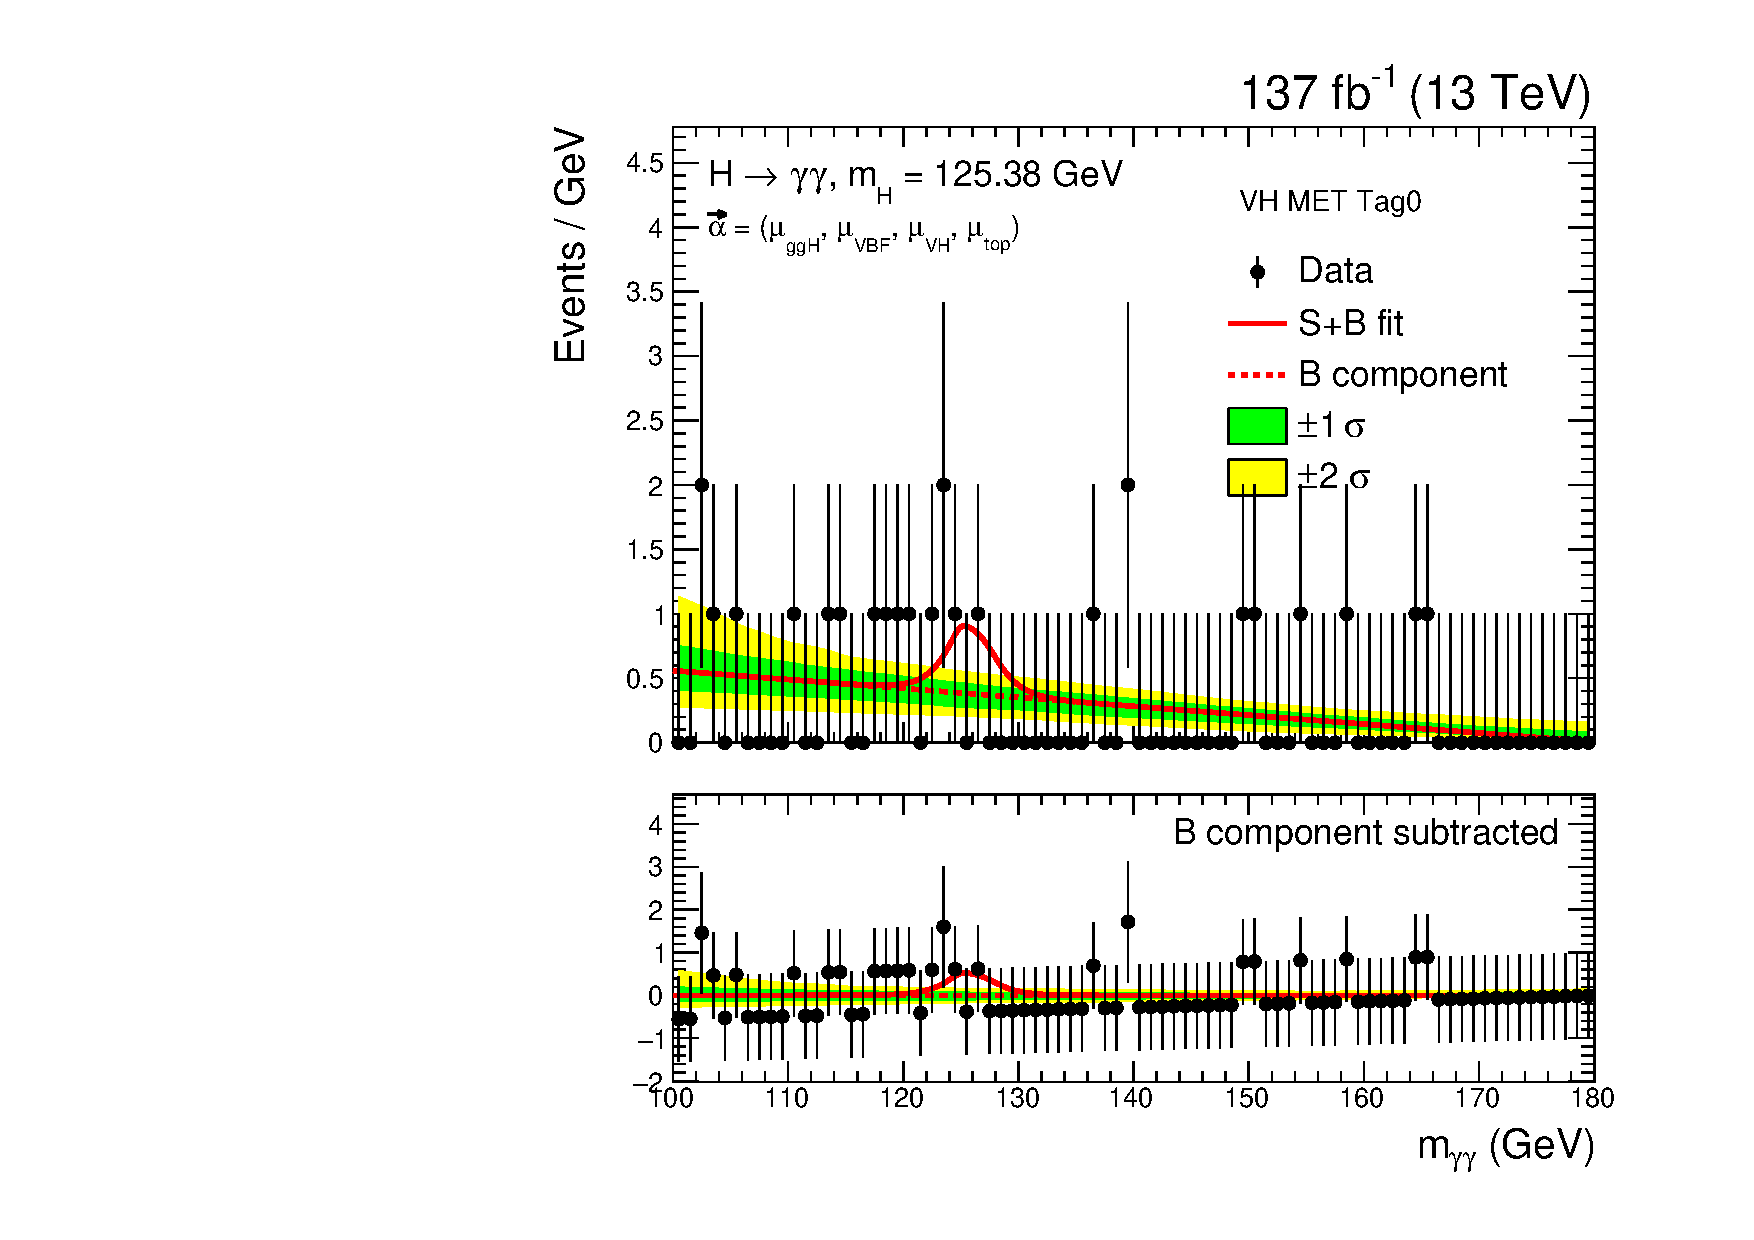
\includegraphics[width=.32\linewidth]{Figures/app_sb_models/RECO_VH_MET_Tag0_CMS_hgg_mass.pdf}
  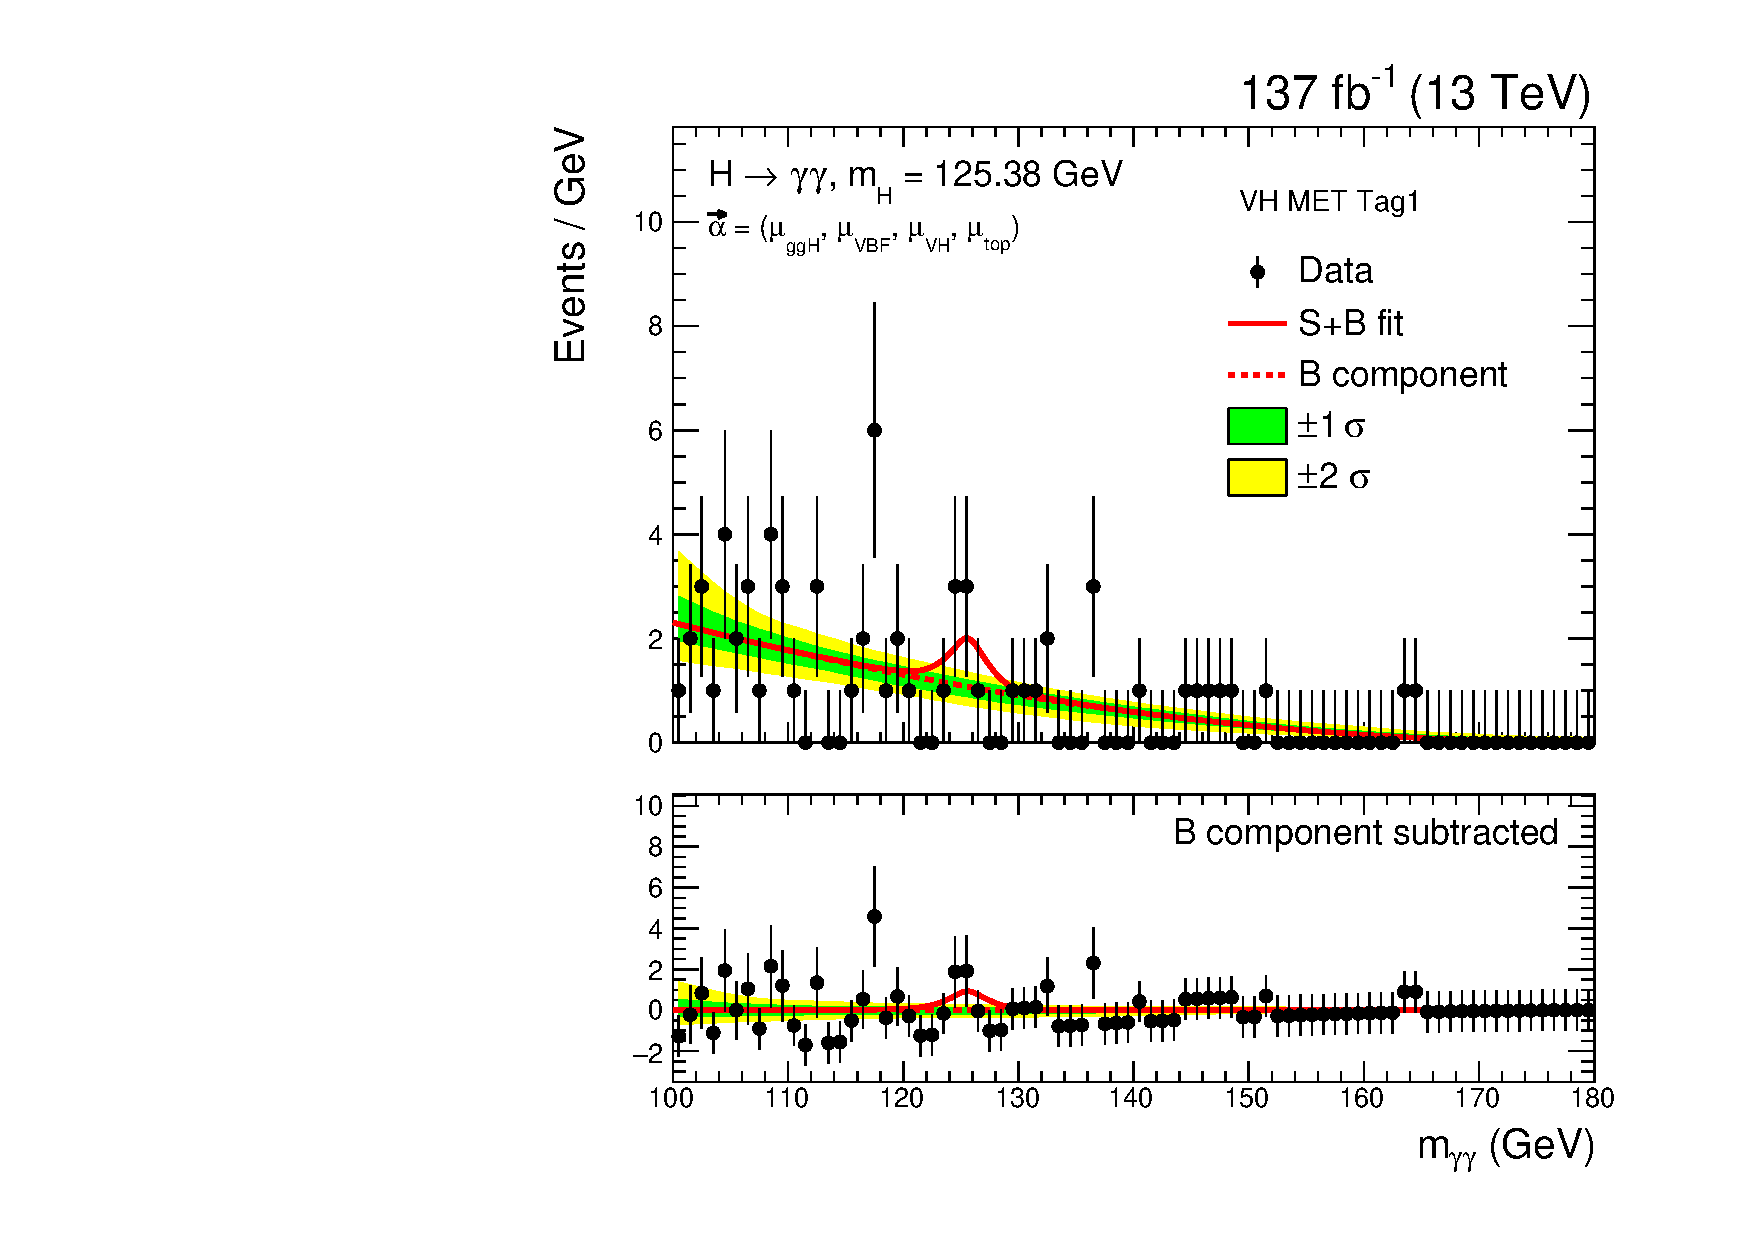
\includegraphics[width=.32\linewidth]{Figures/app_sb_models/RECO_VH_MET_Tag1_CMS_hgg_mass.pdf}
  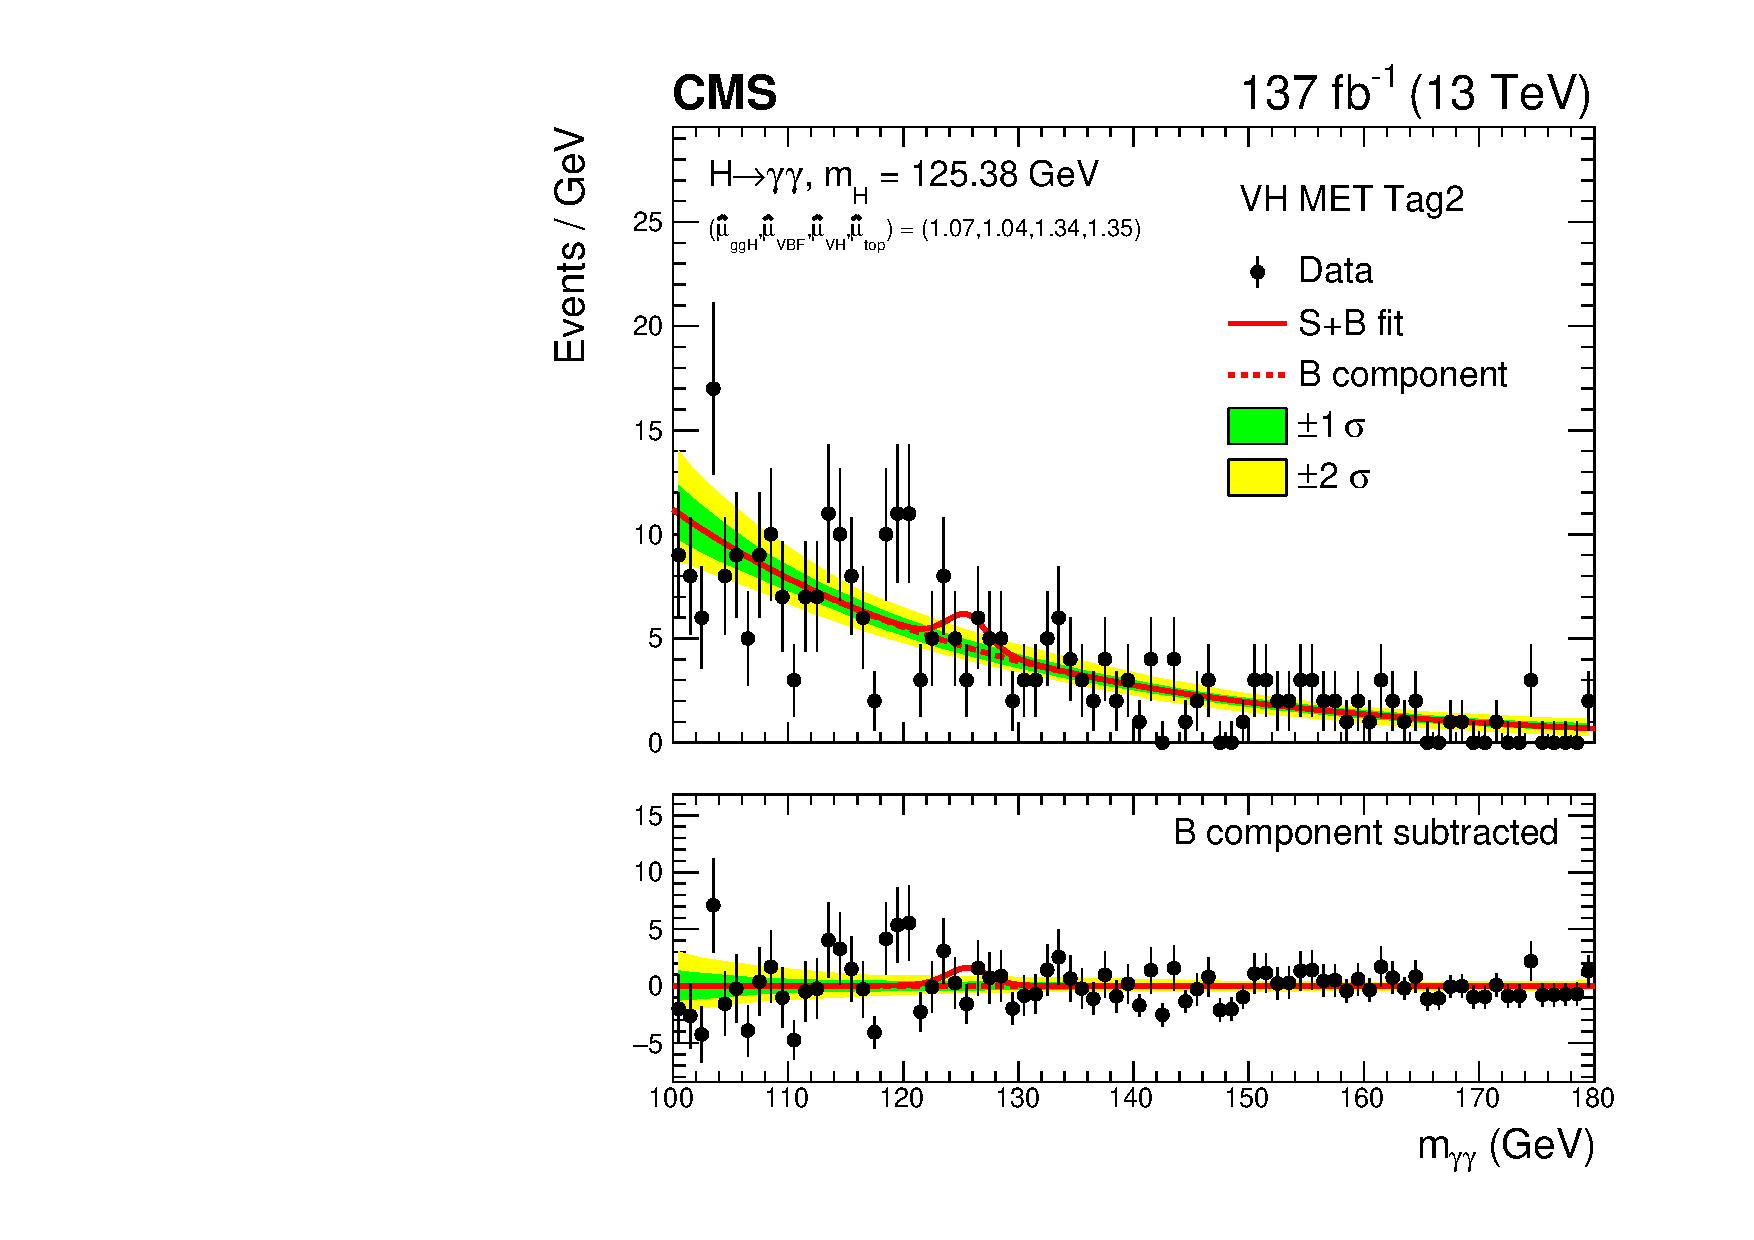
\includegraphics[width=.32\linewidth]{Figures/app_sb_models/RECO_VH_MET_Tag2_CMS_hgg_mass.pdf}
  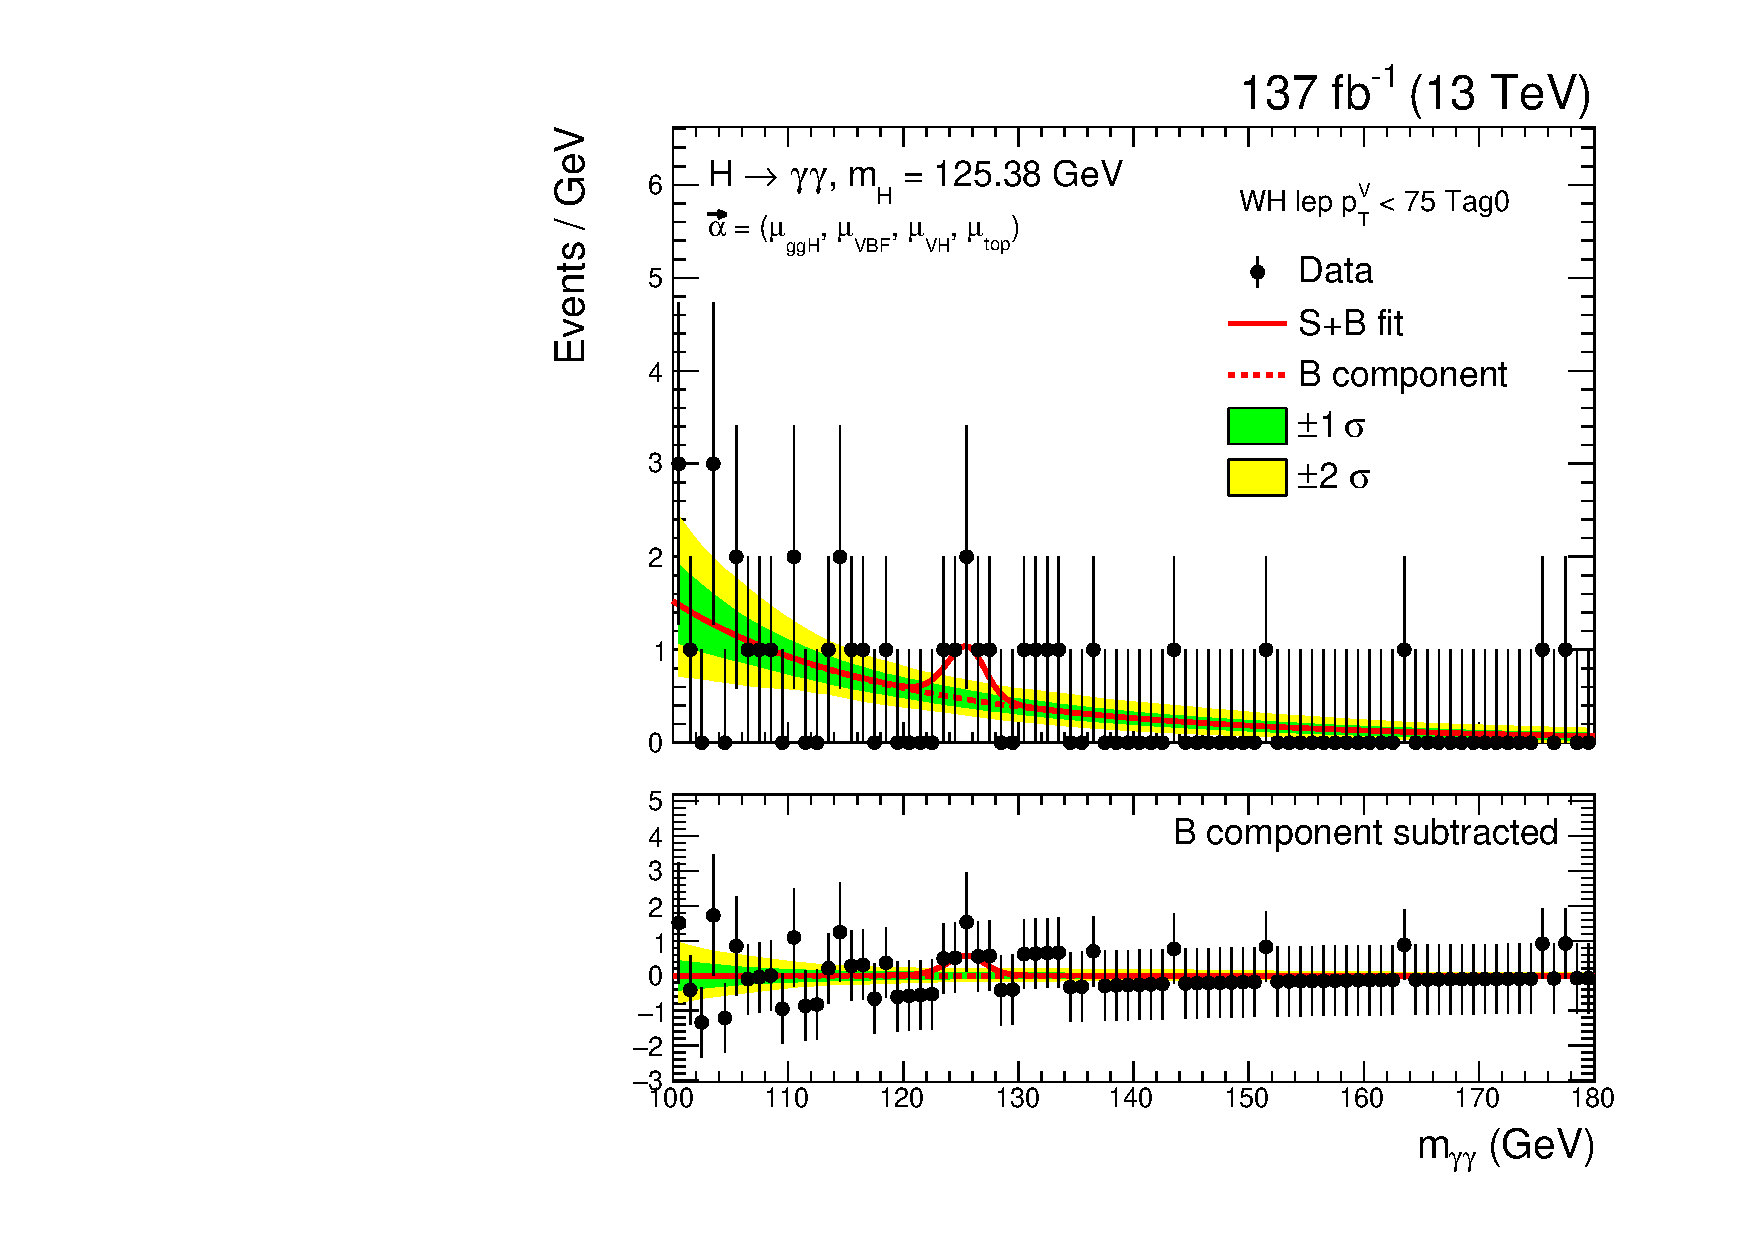
\includegraphics[width=.32\linewidth]{Figures/app_sb_models/RECO_WH_LEP_PTV_0_75_Tag0_CMS_hgg_mass.pdf}
  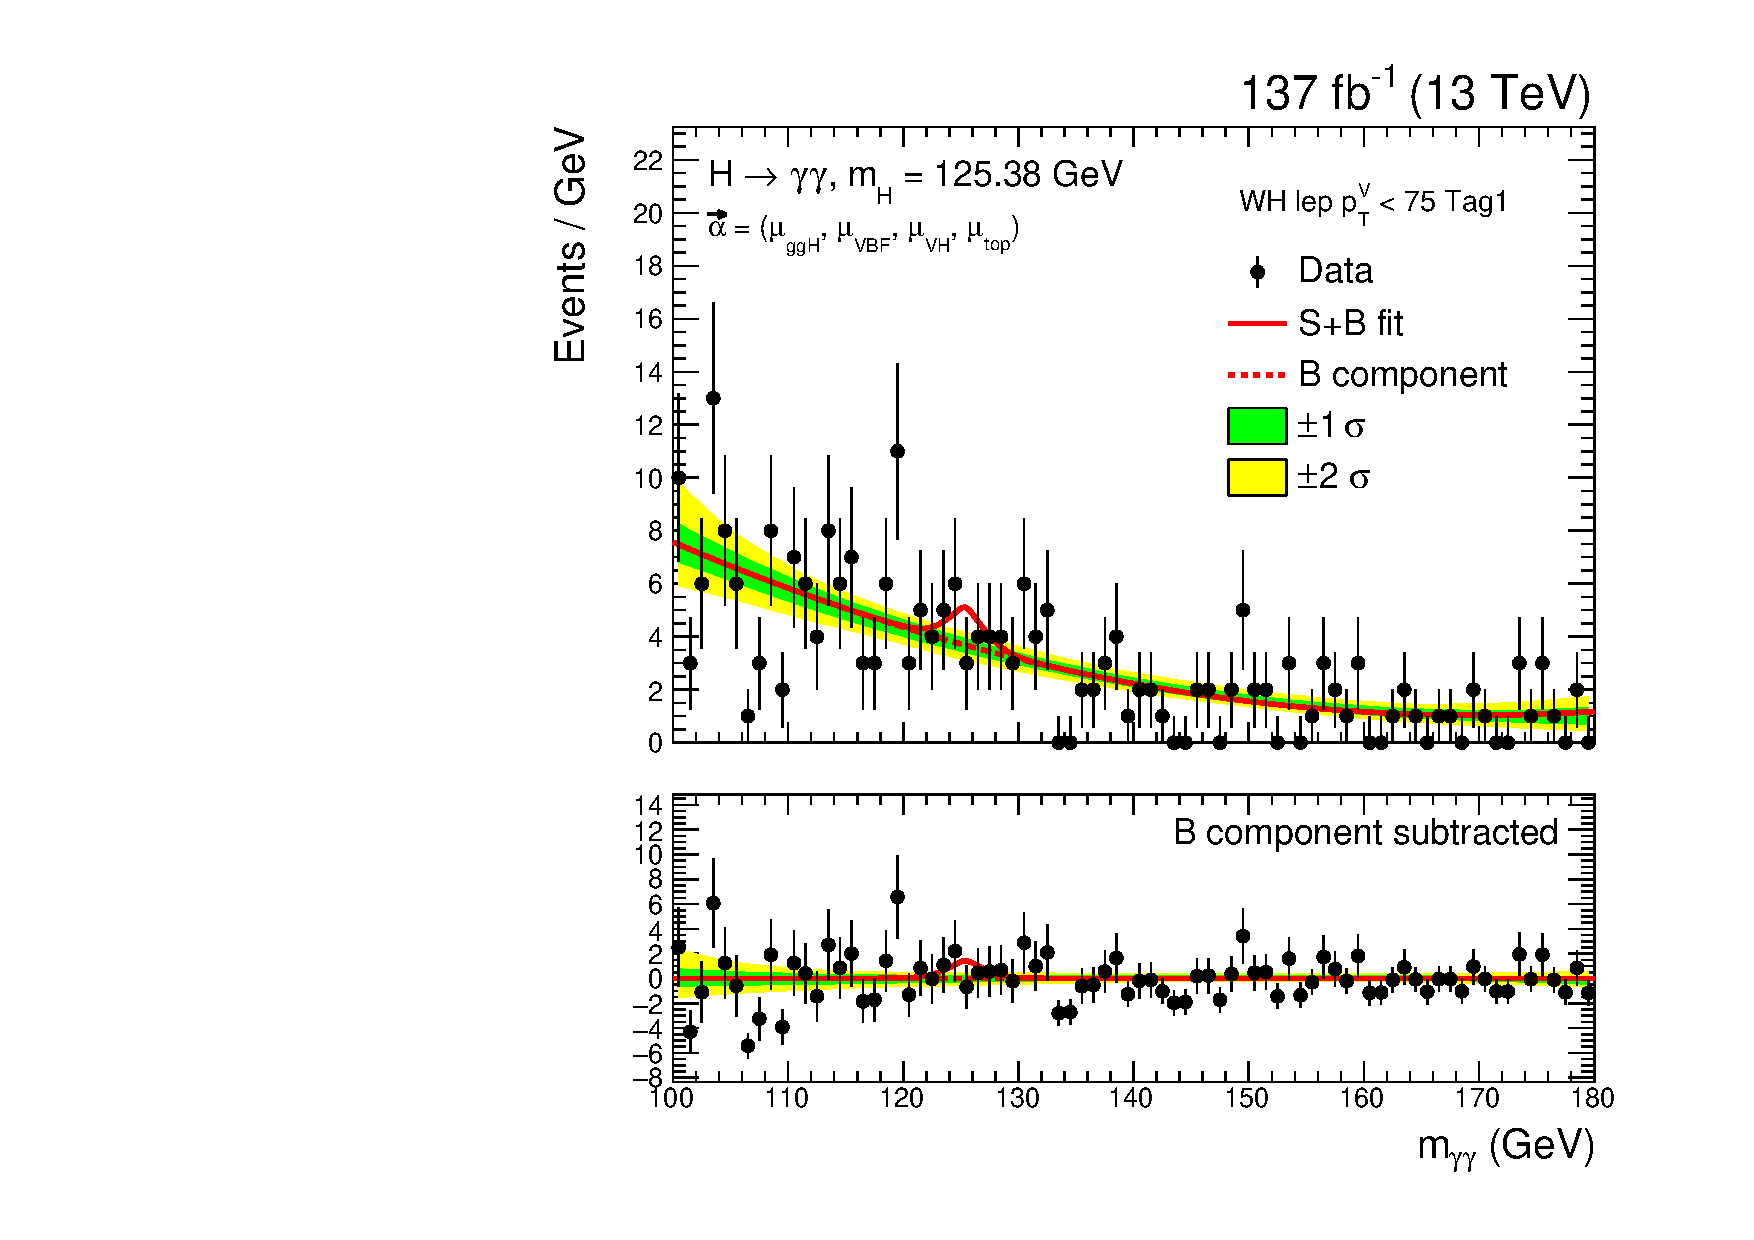
\includegraphics[width=.32\linewidth]{Figures/app_sb_models/RECO_WH_LEP_PTV_0_75_Tag1_CMS_hgg_mass.pdf}
  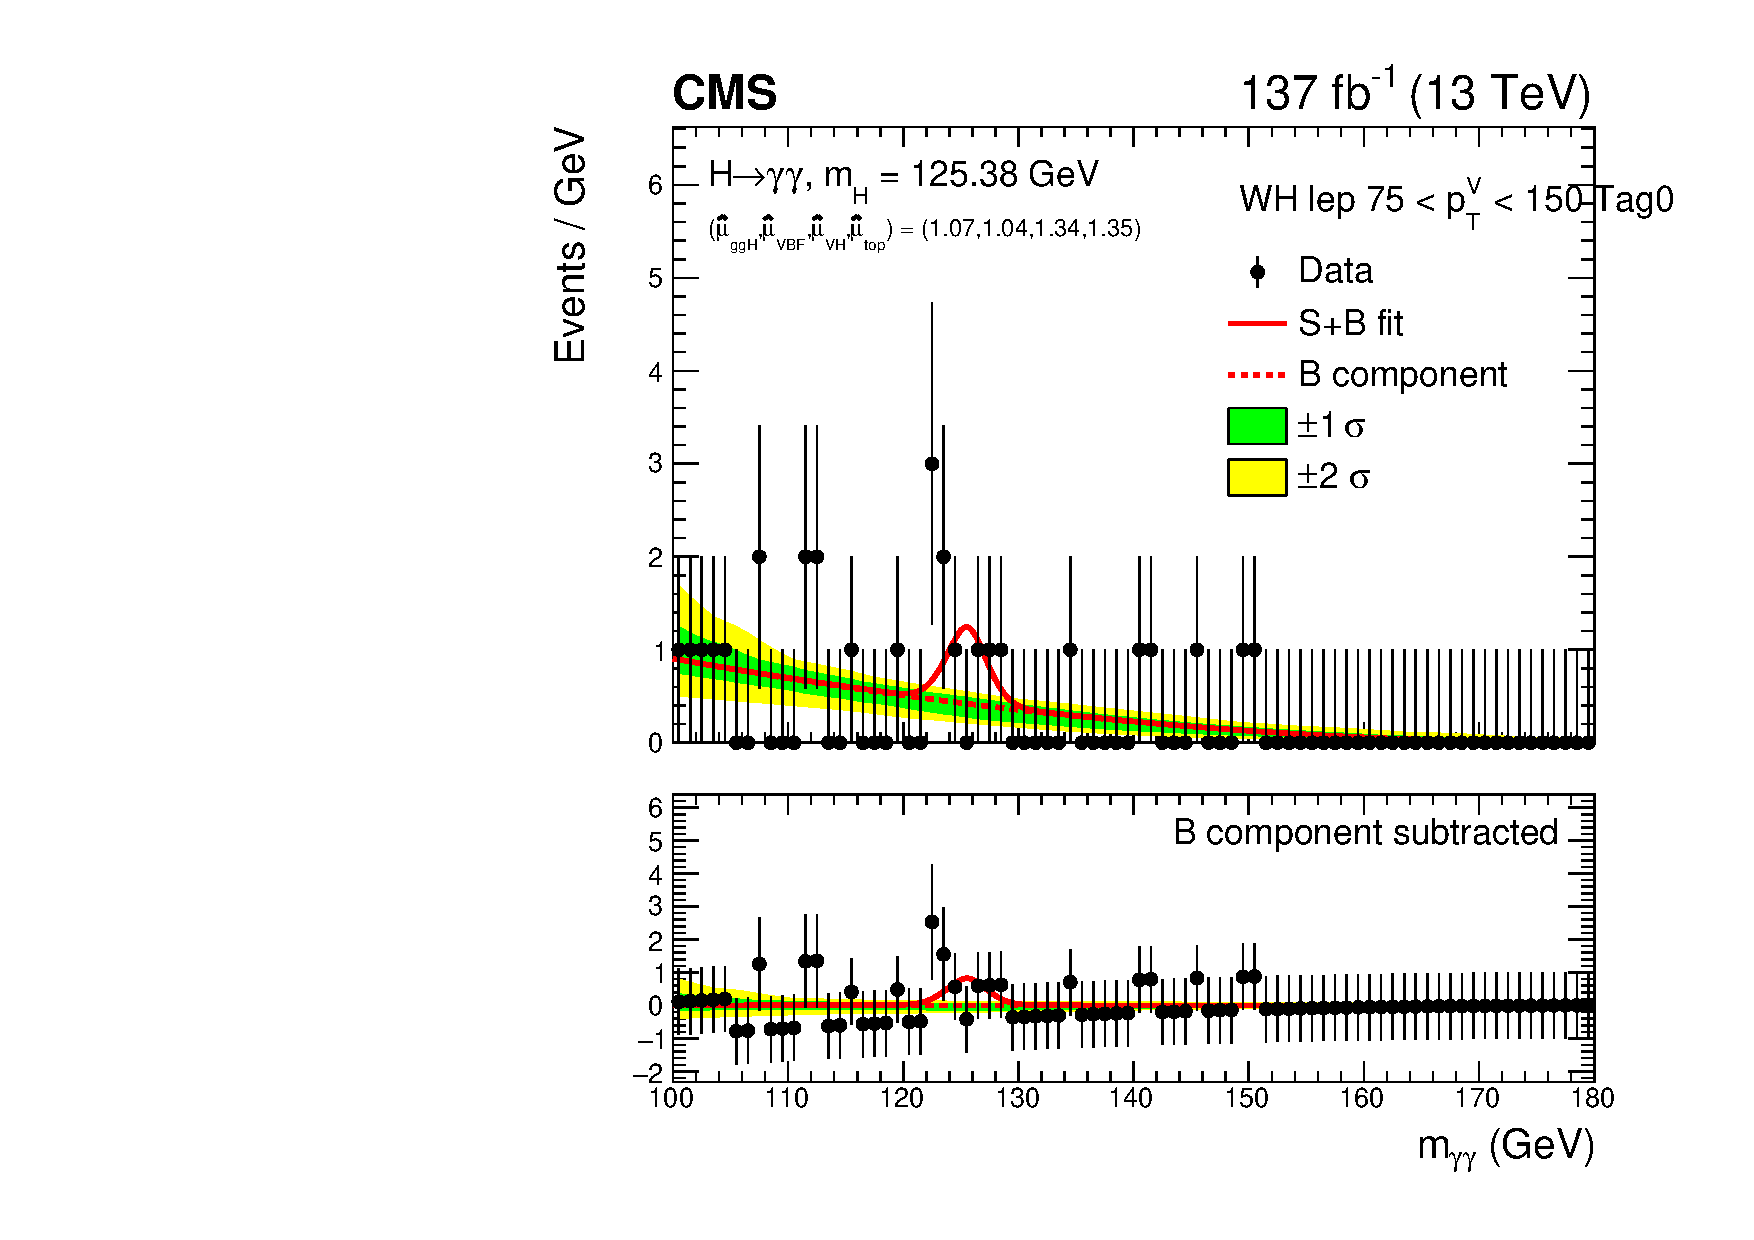
\includegraphics[width=.32\linewidth]{Figures/app_sb_models/RECO_WH_LEP_PTV_75_150_Tag0_CMS_hgg_mass.pdf}
  \includegraphics[width=.32\linewidth]{Figures/app_sb_models/RECO_WH_LEP_PTV_75_150_Tag1_CMS_hgg_mass.pdf}
  \includegraphics[width=.32\linewidth]{Figures/app_sb_models/RECO_WH_LEP_PTV_GT150_Tag0_CMS_hgg_mass.pdf}
  \includegraphics[width=.32\linewidth]{Figures/app_sb_models/RECO_ZH_LEP_Tag0_CMS_hgg_mass.pdf}
  \includegraphics[width=.32\linewidth]{Figures/app_sb_models/RECO_ZH_LEP_Tag1_CMS_hgg_mass.pdf}
  \caption[Observed diphoton mass distributions: VH leptonic]
  {
    Data points (black) and the best-fit signal-plus-background model for the individual analysis categories targeting the VH leptonic STXS regions. The best-fit model corresponds to the per-production mode signal strength fit. The solid red line shows the best-fit signal-plus-background model, whereas the dashed line shows the background component only. The one standard deviation (green) and two standard deviation (yellow) bands show the uncertainties in the background component of the fit. The bottom panels in each plot show the residuals after subtraction of this background component.
  }
  \label{fig:diphoton_mass_4}
\end{figure}

\begin{figure}[htbp]
  \centering
  \includegraphics[width=.32\linewidth]{Figures/app_sb_models/RECO_TTH_HAD_PTH_0_60_Tag0_CMS_hgg_mass.pdf}
  \includegraphics[width=.32\linewidth]{Figures/app_sb_models/RECO_TTH_HAD_PTH_0_60_Tag1_CMS_hgg_mass.pdf}
  \includegraphics[width=.32\linewidth]{Figures/app_sb_models/RECO_TTH_HAD_PTH_0_60_Tag2_CMS_hgg_mass.pdf}
  \includegraphics[width=.32\linewidth]{Figures/app_sb_models/RECO_TTH_HAD_PTH_60_120_Tag0_CMS_hgg_mass.pdf}
  \includegraphics[width=.32\linewidth]{Figures/app_sb_models/RECO_TTH_HAD_PTH_60_120_Tag1_CMS_hgg_mass.pdf}
  \includegraphics[width=.32\linewidth]{Figures/app_sb_models/RECO_TTH_HAD_PTH_60_120_Tag2_CMS_hgg_mass.pdf}
  \includegraphics[width=.32\linewidth]{Figures/app_sb_models/RECO_TTH_HAD_PTH_120_200_Tag0_CMS_hgg_mass.pdf}
  \includegraphics[width=.32\linewidth]{Figures/app_sb_models/RECO_TTH_HAD_PTH_120_200_Tag1_CMS_hgg_mass.pdf}
  \includegraphics[width=.32\linewidth]{Figures/app_sb_models/RECO_TTH_HAD_PTH_120_200_Tag2_CMS_hgg_mass.pdf}
  \includegraphics[width=.32\linewidth]{Figures/app_sb_models/RECO_TTH_HAD_PTH_120_200_Tag3_CMS_hgg_mass.pdf}
  \caption[Observed diphoton mass distributions: ttH]
  {
    Data points (black) and the best-fit signal-plus-background model for the individual analysis categories targeting the ttH STXS regions in the hadronic channel. The best-fit model corresponds to the per-production mode signal strength fit. The solid red line shows the best-fit signal-plus-background model, whereas the dashed line shows the background component only. The one standard deviation (green) and two standard deviation (yellow) bands show the uncertainties in the background component of the fit. The bottom panels in each plot show the residuals after subtraction of this background component.
  }
  \label{fig:diphoton_mass_5}
\end{figure}

\begin{figure}[htbp]
  \centering
  \includegraphics[width=.32\linewidth]{Figures/app_sb_models/RECO_TTH_HAD_PTH_200_300_Tag0_CMS_hgg_mass.pdf}
  \includegraphics[width=.32\linewidth]{Figures/app_sb_models/RECO_TTH_HAD_PTH_200_300_Tag1_CMS_hgg_mass.pdf}
  \includegraphics[width=.32\linewidth]{Figures/app_sb_models/RECO_TTH_HAD_PTH_200_300_Tag2_CMS_hgg_mass.pdf}
  \includegraphics[width=.32\linewidth]{Figures/app_sb_models/RECO_TTH_HAD_PTH_GT300_Tag0_CMS_hgg_mass.pdf}
  \includegraphics[width=.32\linewidth]{Figures/app_sb_models/RECO_TTH_HAD_PTH_GT300_Tag1_CMS_hgg_mass.pdf}
  \includegraphics[width=.32\linewidth]{Figures/app_sb_models/RECO_TTH_LEP_PTH_0_60_Tag0_CMS_hgg_mass.pdf}
  \includegraphics[width=.32\linewidth]{Figures/app_sb_models/RECO_TTH_LEP_PTH_0_60_Tag1_CMS_hgg_mass.pdf}
  \includegraphics[width=.32\linewidth]{Figures/app_sb_models/RECO_TTH_LEP_PTH_0_60_Tag2_CMS_hgg_mass.pdf}
  \includegraphics[width=.32\linewidth]{Figures/app_sb_models/RECO_TTH_LEP_PTH_60_120_Tag0_CMS_hgg_mass.pdf}
  \includegraphics[width=.32\linewidth]{Figures/app_sb_models/RECO_TTH_LEP_PTH_60_120_Tag1_CMS_hgg_mass.pdf}
  \includegraphics[width=.32\linewidth]{Figures/app_sb_models/RECO_TTH_LEP_PTH_60_120_Tag2_CMS_hgg_mass.pdf}
  \caption[Observed diphoton mass distributions: ttH]
  {
    Data points (black) and the best-fit signal-plus-background model for the individual analysis categories targeting the ttH STXS regions, in the hadronic and leptonic channels. The best-fit model corresponds to the per-production mode signal strength fit. The solid red line shows the best-fit signal-plus-background model, whereas the dashed line shows the background component only. The one standard deviation (green) and two standard deviation (yellow) bands show the uncertainties in the background component of the fit. The bottom panels in each plot show the residuals after subtraction of this background component.
  }
  \label{fig:diphoton_mass_6}
\end{figure}

\begin{figure}[htbp]
  \centering
  \includegraphics[width=.32\linewidth]{Figures/app_sb_models/RECO_TTH_LEP_PTH_120_200_Tag0_CMS_hgg_mass.pdf}
  \includegraphics[width=.32\linewidth]{Figures/app_sb_models/RECO_TTH_LEP_PTH_120_200_Tag1_CMS_hgg_mass.pdf}
  \includegraphics[width=.32\linewidth]{Figures/app_sb_models/RECO_TTH_LEP_PTH_200_300_Tag0_CMS_hgg_mass.pdf}
  \includegraphics[width=.32\linewidth]{Figures/app_sb_models/RECO_TTH_LEP_PTH_GT300_Tag0_CMS_hgg_mass.pdf}
  \includegraphics[width=.32\linewidth]{Figures/app_sb_models/RECO_THQ_LEP_CMS_hgg_mass.pdf}
  \caption[Observed diphoton mass distributions: ttH and tHq]
  {
    Data points (black) and the best-fit signal-plus-background model for the individual analysis categories targeting the ttH and tH STXS regions, in the leptonic channel. The best-fit model corresponds to the per-production mode signal strength fit. The solid red line shows the best-fit signal-plus-background model, whereas the dashed line shows the background component only. The one standard deviation (green) and two standard deviation (yellow) bands show the uncertainties in the background component of the fit. The bottom panels in each plot show the residuals after subtraction of this background component.
  }
  \label{fig:diphoton_mass_7}
\end{figure}